%4cm binding margin left
%2cm head margin top
%2.5cm fore-edge margin right
%4cm tail margin  bottom
%a4 is 21 x 29.7 cm

%1.5 spacing for main body, 
%single spacing for bibliography

%% Master tex file for the thesis.

%\documentclass[11pt,a4paper]{book} % double-sided
\documentclass[12pt,a4paper]{report}


\usepackage{subfigure,epsfig,amstext,floatfig,alltt,fancyhdr,setspace,xspace}
\include{macros}
\initfloatingfigs

%%% helps to discourage hyphenation 10000 for no hyphens but dodgy line lengths%%%
\hyphenpenalty=5000
\tolerance=1000

% sets all the margins to be the correct size for thesis

%%%%%%% FINAL THESIS MARGINS  %%%%%%%%%
\setlength{\oddsidemargin}{0.7cm}
%\setlength{\evensidemargin}{1.46cm}
\setlength{\evensidemargin}{-0.04cm}
%\setlength{\evensidemargin}{0cm}
\setlength{\textwidth}{14.5cm}
\setlength{\topmargin}{-0.94cm}
\setlength{\textheight}{21.9cm} %22.2
\renewcommand{\hoffset}{0cm}
\renewcommand{\voffset}{0cm}
%%%%%%%%%%%%%%%%%%%%%%%%%%%%%%%%%%%%%%%



%% In the beginning ....
\begin{document}
%% First do introductory stuff - leave this as pagestyle empty until after
%% the table of contents
%\pagestyle{empty}
%
%\title{
\pagestyle{empty}

\begin{center}
\LARGE
%\vspace*{2cm}
{\bf  Searching for Supersymmetry with the $\alpha_{T}$ variable in $p \bar{p}$ collisions with the CMS Detector at the Large Hadron Collider}

\vspace{1cm}
%\begin{figure}[!ht]

\large
{\it Zoe Hatherell}

\vspace{2cm}
\normalsize
%\begin{center}        
A thesis submitted in fulfilment of the requirements\\
for the degree of Doctor of Philosophy\\
to Imperial College London

December 2011
\end{center}
%\maketitle     


%\ \newpage		% Newpage needed if doing double sided.



%% Include abstract - use separate parskip for this and then set parskip for
%% rest of thesis.
%\pagestyle{plain}

%-----------------------------------------------------------------------------

\pagestyle{fancy}
\fancyhead{} %clear all fields
\renewcommand{\headheight}{28pt}
\cfoot{}
\fancyfoot[LE,RO]{\thepage}

\renewcommand{\chaptermark}[1]{\markboth{\chaptername \ \thechapter.\ #1}{}} 
\renewcommand{\sectionmark}[1]{\markright{\thesection.\ #1} {}}

\fancyhead[LE]{\small \slshape \leftmark}      % Chapter in the right on even pages
\fancyhead[RO]{\small \slshape \rightmark}     % Section in the left on odd pages
\renewcommand{\headrulewidth}{0.3pt}    % Width of head rule

%-----------------------------------------------------------------------------


\pagenumbering{roman}
\setcounter{page}{1}
\newcommand{\lumi}{\mathcal{L}}
\newcommand{\HT}{\ensuremath{H_{T}}}
\newcommand\rs{\raisebox{1.0ex}[-1.0ex]}
\newcommand{\ra}{\ensuremath{\rightarrow}}
\newcommand{\znunu}{\ensuremath{{\text Z} \ra \nu\bar{\nu}}}
\newcommand{\zmumu}{\ensuremath{{\text Z} \ra \mu\mu}}
\newcommand{\wmunu}{\ensuremath{{\text W} \ra \mu\nu}}
\newcommand{\wtaunu}{\ensuremath{{\text W} \ra \tau\nu}}
\newcommand{\dphi}{\ensuremath{\Delta \phi}}
\newcommand{\dphijj}{\ensuremath{\Delta \phi_{ j1,j2}}}
\newcommand{\Pt}{\ensuremath{{p_{\text T}}\xspace}}
\newcommand{\pts}{\ensuremath{p_{\text T}{\text s}}\xspace}
\newcommand{\Et}{\ensuremath{{E_{\text T}}\xspace}}
\newcommand{\ptjf}{\ensuremath{p_{\rm T}^{ {\rm j}_1} }}
\newcommand{\ptjs}{\ensuremath{p_{\rm T}^{ {\rm j}_2} }}
\newcommand{\ptjt}{\ensuremath{p_{\rm T}^{ {\rm j}_3} }}
\newcommand{\etajf}{\ensuremath{\eta^{ {\rm j}_1} }}
\newcommand{\etajs}{\ensuremath{\eta^{ {\rm j}_2} }}
\newcommand{\etajt}{\ensuremath{\eta^{ {\rm j}_3} }}
\newcommand{\ttj}{\ensuremath{\rm{t}\bar{\rm{t}} + jets}\xspace}
\newcommand{\wj}{\ensuremath{\rm W + jets}\xspace}
\newcommand{\zj}{\ensuremath{\rm Z + jets}\xspace}
\newcommand{\al}{\ensuremath{\alpha}}
\newcommand{\alt}{\ensuremath{\alpha_{\text{T}}}\xspace}
\newcommand{\etaabs}{\ensuremath{|\eta|}}
%\newcommand{\gev}{\ensuremath{\mathrm{\,Ge\kern -0.1em V}}}
\newcommand{\pb}{\ensuremath{pb^{-1}}}
\newcommand{\fb}{\ensuremath{fb^{-1}}}
\newcommand{\mjj}{\ensuremath{M_{\text{inv}}^{j1,j2}}}
%\newcommand{\ttbar}{\ensuremath{t\bar{t}}}
\newcommand{\chiznew}{\ensuremath{\chi^{0}}\xspace}
\newcommand{\chipnew}{\ensuremath{\chi^{+}}\xspace}
\newcommand{\sQuanew}{\ensuremath{\tilde{\rm q}}\xspace}
\newcommand{\sGlunew}{\ensuremath{\tilde{\rm g}}\xspace}
\newcommand{\ttNew}{\ensuremath{\rm{t}\bar{\rm{t}}}\xspace}
\newcommand{\tev}{\text{TeV}}
\newcommand{\less}{\ensuremath{<}}
\newcommand{\more}{\ensuremath{>}}
%<TW date="30/10/2010">
%\newcommand{\Et}{E_{T}}
\newcommand{\combIso}{Iso_{\textrm{comb.}}}
\renewcommand{\arraystretch}{1.2}
\newcommand{\bigNum}[2]{#1 \, \times \, 10 \, ^{#2}}
%</TW>

\newcommand{\raT}{\ensuremath{R_{\alt}}}
\newcommand{\RaT}{\ensuremath{R_{\alt}}\xspace}

\def\eslash{{\hbox{$E$\kern-0.6em\lower-.05ex\hbox{/}\kern0.10em}}}
\def\vecmet{\mbox{$\vec{\eslash}_T$}} %missing ET vector
\def\vecet{\mbox{$\vec{E}_\text{T}$}} % ET vector
\def\MET{\mbox{$\eslash_\text{T}$}\xspace}
\def\met{\mbox{$\eslash_\text{T}$}\xspace}
\def\mex{\mbox{$\eslash_\text{x}$}} %missing Ex
\def\mey{\mbox{$\eslash_\text{y}$}} %missing Ey
\def\mepar{\mbox{$\eslash_\parallel$}}
\def\meperp{\mbox{$\eslash_\perp$}}
\def\Zmm{Z \rightarrow \mu\mu}
\def\metvec{\mbox{$\vec{\met}$}\xspace}
\def\metvecrec{\mbox{$\vec{\met}^{\rm rec}$}\xspace}
\def\metvecgen{\mbox{$\vec{\met}^{\rm gen}$}\xspace}
\def\metgen{\mbox{$\met^{\rm gen}$}\xspace}
\def\metparl{\mbox{$\mepar^{\rm rec}$}\xspace}
\def\metperp{\mbox{$\meperp^{\rm rec}$}\xspace}
\def\deltamet{\mbox{$\Delta\met$}\xspace}
\def\pthat{\mbox{$\hat{p}_T$}\xspace}
\def\hslash{{\hbox{$H$\kern-0.8em\lower-.05ex\hbox{/}\kern0.10em}}}
\def\MHT{\mbox{$\hslash_\text{T}$}\xspace}
\def\mht{\mbox{$\hslash_\text{T}$}\xspace}
\def\sumet{\mbox{$\sum \rm{E}_\text{T}$}\xspace}
\def\scalht{\mbox{$H_\text{T}$}\xspace}
\def\etmiss{\mbox{$\eslash_\text{T}$}\xspace}
\def\htmiss{\mbox{$\hslash_\text{T}$}\xspace}
\def\mtt{\mbox{$\rm{M}_\text{T2}$}\xspace}
\def\rmec{\mbox{$R_{\mht/\met}$}\xspace}
\def\bdphi{\mbox{$\Delta\phi^{*}$}\xspace}
\def\bigeslash{{\hbox{$E$\kern-0.38em\lower-.05ex\hbox{/}\kern0.10em}}}
\def\bigmet{\mbox{$\bigeslash_T$}}
\def\bighslash{{\hbox{$H$\kern-0.6em\lower-.05ex\hbox{/}\kern0.10em}}}
\def\bigmht{\mbox{$\bighslash_T$}}
\def\cls{\mbox{CL$_s$}\xspace}
\def\incl{\includegraphics[width=0.49\linewidth]}
\def\inclrot{\includegraphics[angle=90,width=0.47\linewidth]}
\def\INCL{\includegraphics[angle=90,width=0.45\linewidth]}
\def\Incl{\includegraphics[angle=90,width=0.60\linewidth]}




\onehalfspacing

%%\addcontentsline{toc}{chapter}{Abstract}
%\chapter*{Abstract}
\noindent 



\vspace{10mm}
\normalsize




%\ \newpage		% Newpage needed if printing double sided.

%\addcontentsline{toc}{chapter}{Declaration}
%\chapter*{Declaration}

\normalsize
Except where otherwise stated, the research undertaken in this thesis
was the unaided work of the author. Where the work was done in collaboration
with others, a significant contribution was made by the author.


\vspace{20mm}
\hfill {\it Z. Hatherell}

\hfill March 2012







%\ \newpage		% Newpage needed if printing double sided.

\addcontentsline{toc}{chapter}{Acknowledgements}
%\chapter*{Acknowledgements}

%\noindent

\normalsize

I would like to extend my thanks to everyone who worked with me and helped me in the course of this Ph.D. I am sincerely and heartily grateful to my advisor, Jordan Nash, for the support and guidance he showed me throughout my time at Imperial College.

It has been a pleasure to be a member of the Imperial RA1 team alongside Rob Bainbridge, Burt Betchart, Oliver Buchm\"uller, Darren Burton, Edward Laird, Bryn Mathias, Henning Fl\"acher, Tanja Rommerskirchen, Paris Sphicas, Markus Stoye, and Tom Whyntie. It would also not have been possible without Georgia Karapostoli, for teaching me so much in the beginning. 

I am grateful to everyone who contributed to the design, construction and running of both the LHC and CMS, without who I would not have had data to analyse. It has been an honour to work at CERN and be part of such an incredible feat of science and engineering.

My heart goes out to everyone I met at CERN, and who made my time there so special. To all the wonderful UK LTA crew who are too numerous to name individually. Collectively you made my time at CERN the best time of my life and I one I will never forget. Special thanks to the LTA ladies for girly nights! 

Many thanks to  my parents Jan and Adrian, who have supported me through everything I have been through for my whole life and taught me that anything is within my grasp. Thanks for always believing in me and being there when the times were toughest. Finally a special thanks to Chris, for all the love and support without which I would not have made it though these months of writing. 



\singlespacing

%\ \newpage		% Newpage needed if printing double sided.

%\addcontentsline{toc}{chapter}{Contents}
%\tableofcontents

%\ \newpage		% Newpage needed if printing double sided.
%\ \newpage		% Newpage needed if printing double sided.

%%%%%ZOE%\addcontentsline{toc}{chapter}{List of figures}
%%%ZOE\listoffigures

%\ \newpage		% Newpage needed if printing double sided.

%%%%ZOE\addcontentsline{toc}{chapter}{List of tables}
%%%%ZOE\listoftables
  
%\ \newpage		% Newpage needed if printing double sided.
%\ \newpage		% Newpage needed if printing double sided.

%%%ZOE\clearpage % this command stops table page becoming page 1


%% Now the body of the text - note that parskip has to be reset after the TOC

\onehalfspacing
\pagenumbering{arabic}

\setcounter{page}{1}
%% Add chapters here %%
%\setcounter{equation}{0}
\setcounter{figure}{0}
\setcounter{table}{0}

\chapter{\label{chapter1} Introduction}

At the heart of science is the quest to further mankind's knowledge of the universe we live in. The Standard Model of particle physics is one of the greatest achievements in this effort, forming the basis of a description of the most fundamental building blocks of nature. However, despite its many successes verified in experimental physics, there are many indications that it is not a complete theory. 

As particle physicists look inwards to smaller scales with higher energies, cosmologists look outwards into space. Cosmological experiments confirm that the matter of the observable universe accounts for only 4\% of the mass in the universe. Another type of matter, known as ``Dark Matter", accounts for 23\% and yet there is no particle in the existing Standard Model to account for this, indicating new physics.  Supersymmetry, one well-motivated possible extension of the Standard Model predicts a new symmetry in which each known particle has an as-yet undiscovered partner. Under an assumption common to many SUSY models, the the lightest of these new particles is stable and weakly interacting, and therefore could account for dark matter. 

Experimental particle physics pushes the frontier of energy ever upwards in order to probe the heart of matter to better resolution. The Large Hadron Collider is the first collider that can access physics on the TeV scale, where many hope the first indications of physics behind the Standard Model will lie. The Compact Muon Solenoid detector will collect data during these proton-proton collisions for analysis in many areas of possible new physics. 

Motivated by Supersymmetry, this thesis details the search for signs of new physics consistent with a dark matter candidate particle. Events are required to have jets and missing energy where the candidate particle escapes the detector. The search is model independent whilst motivated by SUSY, in order to remain sensitive to any new physics resulting in a dark matter candidate particle. 

The Standard Model theory is presented in Chapter~\ref{ch:theory} along with motivations for physics beyond, and a description of Supersymmetry. The data used is taken using the Compact Muon Solenoid Detector at the Large Hadron Collider, experimental descriptions of which are found in Chapter~\ref{ch:detector}, and the reconstruction performed prior to data release for the analysis users is described in Chapter~\ref{ch:objects}.


Chapter~\ref{ch:at} documents the design and verification of the novel background rejection variable \alt, using work undertaken by the author's analysis group in previous iterations of the analysis, and work on the leptonic definition undertaken by the author described in Section~\ref{sec:lalt}. The work presented in Chapter~\ref{ch:ra1} is documented in a public CMS Physics Analysis Summary~\cite{1fbnote} and was published in Physical Review Letters~\cite{PRL1fb} in 2011. The work was undertaken by a small analysis group of which the author was a key active member singularly responsible for the muon control sample used for background prediction and in addition providing plots and yields for the signal selection. The work in Chapter~\ref{ch:ra4} represents an extension to the published analysis that is the sole work of the author, using the aforementioned leptonic definition of the \alt variable. 

Throughout this thesis the use of ``natural" units is employed, such that the Plank constant, the speed of light and the Boltzmann constant are normalised to unity, i.e. $\hbar = c =  k_{B} = 1$. The quantities of mass and energy are then both expressed using the unit ``electron volt"\,(\,eV\,), defined as the energy gain of a single electron charge moving through the potential of one volt, 1.60 $\times 10^{-19}$\,J. Temperature and length may also be written in this convention, but in this thesis are always expressed in the SI units of Kelvin, K, and metres, m. 
\chapter{Theoretical Overview}
\label{ch:theory}
 
The field of particle physics pertains to the attempt to build a full description of the dynamics of the fundamental particles and interactions which govern the universe. Progress is made through both theoretical postulation and experimental finding. The theoretical branch seeks to describe mathematically the framework that reflect the symmetries in nature through the construction of models, both to describe observed behaviour and to predict that not yet observed. The description of current understanding is collectively known as the Standard Model (SM), and is a rigorously tested and widely accepted theory. However, whilst there are no disagreements, there are some gaps which hint at physics beyond, fuelling many new theories that predict new physics beyond. This leads in turn to a  new generation of experimentalists seeking answers to what lies at the next energy frontier.

\section{The Standard Model}

The Standard Model (SM) is the name given to the theories that successfully describe the known elementary particles and their fundamental interactions with respect to the strong, weak and electromagnetic forces. Within it there are two main types of fundamental particle, which in order to distinguish requires the introduction of the concept of spin.

\begin{description}
\item[Spin] \hfill \\
Spin is the name given to a property of elementary particles, corresponding to a type of angular momentum, although this differs from classical angular momentum. This is an intrinsic property and thus has a specific value for each particle type. It can be thought of for massive particles as the angular momentum about the central point, but it is known that massless particles such as the photon carry spin also, so this analogy breaks down. The values of the spin quantum number s which describe the magnitude can take any half integer value $s=0, \frac{1}{2}, 1, \frac{3}{2}$, etc. In addition to magnitude we describe a particle as having spin \textit{up} (positive) when the spin is in the direction of the z-axis, and spin \textit{down} (negative) if the spin is against the direction of the z-axis. 

The definition of spin gives rise to a second key property, known as chirality. When the spin direction is in the direction of momentum of the particle it is described as left-handed, and when it is against as right-handed. The chirality of a particle is integral to the way it behaves, as will be seen in the treatment of the weak force. In the massless limit  the chirality is analogous to another concept, that of helicity, although it is worth noting that for a massive particle helicity depends on the reference frame of observation, wheres chirality describes an inherent property that determines how the particle will behave.
\end{description}
All fundamental particles are divided into the spin-1/2 \textit{fermions} which are the building blocks for matter, and the force-mediating \textit{bosons} which must carry integer spin, usually spin-1.  A particle's spin dictates how it behaves, as the wave function of a bosonic system is symmetric under the swap of two of its particles, whilst that of a fermionic system is anti-symmetric. A consequence of this, as can be seen in Equation \ref{eqn:pauli} is the well-known Pauli Exclusion Principle, that two fermions may not exist in the same state. 

\begin{equation}
\psi_{f}(x_{a},x_{b}) = -\psi_{f}(x_{b},x_{a}), \quad \therefore \quad \psi_{f}(x_{a},x_{a}) = 0
\label{eqn:pauli}
\end{equation}
 

All visible matter is made out of fermions, which can be described in three families, or ``generations", each of which is further divided into two sets, the quarks and the leptons. There are three charged leptons with one unit (negative) of electric charge, e, the electron (e$^{-}$), the muon ($\mu^{-}$) and the tau ($\tau^{-}$), and three associated massless or incredibly light  neutral leptons called neutrinos that are named after the charged lepton in their generation, $\nu_{e}$, $\nu_{\mu}$ and $ \nu_{\tau}$ respectively. This indicates the introduction of a new concept, ``flavour", of which there are three, one for each generation. 

The quarks show an analogous structure, divided into two types dependent on electric charge carried, each with three generations. The up (u), charm (c) and top (t) quarks carry $+\sfrac{2}{3}$ e while the down (d), strange (s) and bottom (b) quarks carry $-\sfrac{1}{3}$ e. Each of the 6 quarks corresponds to its own flavour. 

The generation structure is shown in Equation~\ref{eqn:threefams}. The particles in the second and third generation exhibit the same properties as the corresponding first generation particles, except for the mass which increases with ascending generations. The first generation is therefore stable and all ordinary matter is constructed from it, whilst the second and third, once produced, decay into particles of the first generation. In addition to each particle detailed here, there exists a corresponding antiparticle due to a symmetry in charge and quantum numbers.  Each fermion can be described as a spinor field $\psi$ which describes a pair of complex fields, the left-handed ($\psi_{L}$) and right-handed ($\psi_{R}$) representations. 
 
\begin{equation}
\begin{bmatrix}
\nu_{e} & u \\
e & d \\
\end{bmatrix},
\begin{bmatrix}
\nu_{\mu} & c \\
\mu & s \\
\end{bmatrix},
\begin{bmatrix}
\nu_{\tau} & t \\
\tau & b\\
\end{bmatrix}
\label{eqn:threefams}
\end{equation}

The bosons are force mediating particles, the photon $\gamma$ for the electromagnetic force, the 8 gluons $g_{i}$ for the strong force and the $W^{\pm}$ and Z bosons that carry the weak (nuclear) force, all of which are spin-1 particles. The photon and gluons are massless, whilst the weak vector bosons have non-negligible mass. The final particle of the SM is the Higgs Boson of spin-0, as yet undiscovered in experiment but expected from the theory, as will be detailed later. 

\subsection{Gauge Theory of Interactions}

The theories that make up the SM are formulated mathematically using Quantum Field Theory (QFT), in which particles are thought of as excitations of fields, and the dynamics of a given system are summarised in what is known as Lagrangian formalism. In this the Lagrangian L is the difference between kinetic energy T and potential energy V, $L = T - V$. In QFT it is usual to describe a system by the Lagrangian Field Density $\Lagr$, where L is obtained from $\Lagr$ by integrating over the spatial component $d^{3}x$.


In order to reflect the symmetries observed in nature, the dynamics of a system and therefore the Lagrangian Density $\Lagr$, must be invariant under some set of transformations,

\begin{equation}
\psi \rightarrow e^{-i\alpha}\psi, 
\label{GlobalTrans}
\end{equation}


where $\psi$ represents a spinor field. If $\alpha$ has no reliance on the space-time coordinate, we say this is a global symmetry. In order to describe the fundamental interactions it is necessary to use the special case where the transformations are \textit{local}, where $\alpha$ has a dependence on the space-time coordinate. The Standard Model describes such symmetries, a case we call gauge invariance, and is a special case of field theory known as Gauge Theory, where the transformations have the form, 


\begin{equation}
\psi(\stc) \rightarrow e^{-i\alpha(\stc)}\psi (\stc).
\label{LocalTrans}
\end{equation}


It is clear that $\Lagr$ will not remain unchanged by such a transformation, as the dependence of $\alpha$ on $x$ means that the coordinate derivative $\partial_{\mu}$ introduces extra terms. In order to leave the Lagrangian unchanged a vector field is introduced $A_{\mu}$ that transforms under another local transformation to keep $\Lagr$ constant: 

\begin{equation}
A_{\mu} \rightarrow A_{\mu} + \frac{1}{g} \partial_{\mu} \alpha(\stc).
\label{ATrans}
\end{equation}

Thus we can rewrite $\Lagr$ introducing the \textit{covariant derivative}, 
\begin{equation}
\slashed{\Dev}_{\mu} = \partial_{\mu} - igA_{\mu}. 
\end{equation}

This interaction between the spinor field and the vector field through this covariant derivative indicate the interactions of matter particles though the force carrying bosons. From Noether's Theorem, it is known that as a consequence of a symmetry in a dynamical system there is an associated physically conserved quantity~\cite{Rolnick}. Just as the classical conservation laws pertaining to momentum and energy are given by the space-time translational symmetries in Classical Mechanics, for the electromagnetic force symmetries in Quantum Mechanics the electric charge is conserved. Analogously, there ought to be conserved ``charges" for the strong and weak forces also, corresponding to quantum numbers from their Lagrangian Densities. 
 
The set of possible transformations is described in the language of Group Theory, and thus we describe the SM as a non-Abelian Yang-Mills type gauge field theory based on the symmetry group $SU(3)_{C} \times SU(2)_{L} \times U(1)_{Y}$. As this group is a product, the three individual elements are free to each have their own coupling constant, and these may differ. The strong interactions described by Quantum Chromodynamics (QCD) are represented by $SU(3)_{C}$, labelled C to indicate the conserved charge ``Colour". The electromagnetic and weak interactions are represented together due to Electroweak Unification, which we shall explore in detail later, by the group $SU(2)_L \times U(1)_{Y}$ where L stands for left, indicating the parity violation of the weak interaction and Y the conserved charge ``hypercharge". As of yet, the fourth fundamental force Gravity is not included in the Standard Model, but this is seen as of little consequence to particle physics as gravitational forces have comparatively little effect on fundamental particles at current experimental energy scales. 

\subsubsection{Quantum Electrodynamics}

The fundamental electromagnetic force is studied in quantum field theory as Quantum ElectroDynamics (QED), the oldest and simplest of the theories brought together to form the SM. The symmetry group of QED is U(1) and this gives an associated conserved quantity, the electric charge Q. The electromagnetic force is carried by the massless boson, the photon, and affects only the charged fermions. The symmetry allows no self interaction of the photon. The fermion field $\psi_{q}$ with charge $q$ and mass $m_{q}$ with symmetries under the group of transformations $e^{-i\alpha(\stc)}$ gives rise to the Lagrangian in Equation \ref{eqn:QEDL}.
\begin{equation}
\Lagr_{QED} = \bar{\psi}_{q}(\stc)(i \gamma^{\mu}\mathcal{D}_{QED} - m_{q}) \psi_{q}(\stc) - \frac{1}{4}F_{\mu \nu}F^{\mu \nu}
\label{eqn:QEDL}
\end{equation}

The kinetic term depends on the Field Strength Tensor $F$, 
\begin{equation}
F_{\mu \nu} (\stc) = \partial_{\mu} A_{\nu}(\stc) -   \partial_{\nu} A_{\mu}(\stc) 
\end{equation}

which incorporates the introduction of a gauge field $A_{\mu}$ which is transformed along with $\psi$ in the following way:

\begin{equation}
A_{\mu}(\stc) \rightarrow A_{\mu}(\stc) + \partial_{\mu} \alpha(\stc)
\label{AQED}
\end{equation}

The  covariant derivative, $\slashed{D}_{QED,\mu}$ is defined as in Equation \ref{eqn:QEDD} so as to maintain an invariance to local U(1) charge symmetry. 
\begin{equation}
\slashed{\mathcal{D}}_{QED} = \partial_{\mu} + iqA_{\mu}
\label{eqn:QEDD}
\end{equation}


where q is described as the generator of the symmetry group and is analogous to electric charge. The strength of coupling of each force is described by the coupling constant, in this case governed by the constant e, the charge of an electron: $\alpha = \frac{e^{2}}{4\pi}$. This is more commonly known as the \textit{fine structure constant} and has been measured experimentally to a high degree of accuracy to have a value $\alpha \sim \sfrac{1}{137}$ \cite{qedalpha}. The coupling constants of the standard model are not fixed at all energy scales, rather they vary, and this is called the ``running" of the coupling constants. This will become important when incorporating the other forces. 

\subsubsection{QCD}

Quantum Chromodynamics (QCD) is the relevant quantum field theory that describes the dynamics of the strong force. The strong force of symmetry group $SU(3)_{C}$ has 8 massless gauge bosons known as the gluons, and a conserved quantity called colour charge, which has three types called $q_{i},$ where $i=1, 2, 3$. The name ``colour" is not meant to imply a connection to visual colour, merely an analogy between the three types and the primary colours red, blue and green. Only particles which carry colour charge are affected - the quarks have colour, while leptons do not. Unlike the photon in electromagnetism, the gluons that mediate the force carry the charge also, leading to the self-interactions that govern the behaviour of QCD. 

A quark carries one ``colour" $q_{i}$, taking one of the three possible values, and an analogous antiquark carries one ``anti-colour". On the other hand, gluons carry both a colour and an anti-colour.  Separation of two charges gives rise to a potential energy, which increases linearly as the charges are moved further apart. As a consequence, it would take an infinite amount of energy to separate two quarks, and thus they are not found free in nature, but only bound within colourless composite particles, an effect called \textit{confinement}. There are two observed stable bound states, the three-quark hadrons such as the proton p $\sim$ uud and the neutron n $\sim$ udd, and quark-anti-quark mesons such as the pions $\pi^{0}, \pi^{\pm}$. This explains why colour charge is not observed in nature, as measured beyond a fundamental distance it is required to be zero.

The local SU(3)$_{C}$ invariance of QCD is defined by the transformations in Equation \ref{eqn:qcdtrans}, where $g_{s}$ is the strong coupling constant, $\lambda_{\alpha}$ are the Gell Mann matrices, and the $\theta^{\alpha}$ describe the transformation angles. 

\begin{equation}
q(\stc) \rightarrow e^{i\frac{g_{s}}{2}\theta^{\alpha}(\stc) \lambda_{\alpha}} q(\stc) \quad \mathrm{with} \quad \alpha = 1, ... , 8
\label{eqn:qcdtrans}
\end{equation}


As with QED, the gauge fields of the gluons $A^{\alpha}_{\mu} $ also transform as in Equation \ref{eqn:qcdA} to maintain local invariance. 
\begin{equation}
A^{\alpha}_{\mu}(\stc) \rightarrow A^{\alpha}_{\mu}(\stc) = \frac{1}{g_{s}} \partial_{\mu}\theta^{\alpha}(\stc) + f_{\alpha \beta \gamma}\theta^{\beta}(\stc)A^{\gamma}_{\mu}(\stc)
\label{eqn:qcdA}
\end{equation}


The Lagrangian for a quark carrying colour $\alpha$ is then described in Equation \ref{eqn:QCDL}

\begin{equation}
\Lagr_{QCD} = \sum_{q} \bar{q}(i \gamma^{\mu}\slashed{D}_{QCD} - m_{q}) q - \frac{1}{4}G^{\alpha}_{\mu \nu}G^{\mu \nu}_{\alpha}
\label{eqn:QCDL}
\end{equation}

where the covariant derivative in this case is


\begin{equation}
\slashed{\Dev}_{QCD} = \partial_{\mu} - i\frac{g_{S}}{2}\lambda_{\alpha}A^{\alpha}_{\mu}(\stc)
\label{eqn:QCDD}
\end{equation}

The gluon field tensor $G^{\alpha}_{\mu \nu}$, analogous to the photon field tensor that was seen in QED is defined in Equation \ref{eqn:GQCD}. Unlike that of the photon, it can be seen that in the kinetic term of $\Lagr$ this gives rise to three and four gluon terms thus describing the self-interaction of the gluons. 

\begin{equation}
G^{\alpha}_{\mu \nu} (\stc) = \partial_{\mu} A^{\alpha}_{\nu} (\stc) - \partial_{\nu}A^{\alpha}_{\mu}(\stc) + g_{S} f_{\alpha \beta \gamma} A^{\beta}_{\mu}(\stc)A^{\gamma}_{\mu}(\stc)
\label{eqn:GQCD}
\end{equation}



 To describe the behaviour of the strength with decreasing distance, we define an analogous coupling constant for the strong force to that in QED, which we call $\alpha_{S} = \sfrac{g_{S}^{2}}{4\pi}$. Whilst its QED equivalent runs weaker as the distance between charges increases, as we have discussed the strong force has the opposite relationship, reflected in the running of the coupling constants with increasing energy scale, which when extrapolated could highlight an energy scale where the two are equal. When we discuss quarks in particle physics although they are free, this is as a result of the ``asymptotic freedom" where when viewed at very large energies the distances are infinitely small, and the quarks behave freely. 
 
 \subsubsection{The Parton Model}
 
 In order to understand the physics at hadron-colliders, Feynman introduced the Parton Model, a description of the way the partons (quarks and gluons) inside a hadron behave. The behaviour depends on the energy at which the collision occurs. Each of the quarks in a hadron is joined to the other two by continually exchanging gluons and changing colour in such a way that the bound state remains colour neutral. However, as the distance between a pair of quarks is extended the colour field is put under stress until the gluon splits in two, and in between them a quark-anti-quark pair is created. The three quarks which define the hadron are known as the \textit{valence quarks} and those that appear in these pairs are known as the sea quarks. Gluons can also be created, through the annihilation of such a pair of sea quarks, and these processes go on continually within hadrons. 
 
 When colliding at low energies, the system behaves as three separate valence quarks with a certain fraction of momentum each, but at higher energies the sea quarks must be taken into account also, as they can possess a significant fraction of energy.  Thus physics at hadron colliders is more complicated than lepton colliders, as it is not trivial to understand the two particles that interact, or the energy that they collide at. Thus it is necessary to know the probability that a given parton has a certain fraction of the energy of the hadron,  described by a Parton Distribution Function (PDF). The PDFs for high energy hadron collisions cannot be calculated theoretically, as inclusion of all potential combinations of sea quarks is not possible due to the non-perturbative nature of QCD caused by the large coupling constant $\alpha_{S}$. Thus these are measured experimentally by collaborations such as CTEQ~\cite{CTEQ}. 
 


\subsubsection{The Weak Force and Electroweak Unification}

The weak interaction, responsible for radioactive decay, makes up the final piece of the puzzle. So named because of its relatively low strength compared to the electromagnetic and strong forces, it is was theorised as being mediated by massive force bosons $W^{\pm}$ and Z long before they were discovered experimentally. A lagrangian theory for the weak force must take into account the characteristics of weak interactions. The group symmetry is SU(2) giving rise to a conserved quantity known as weak isospin, I which has a component $T_{3}$ that points in the direction of the z axis. The left-handed fermions form isospin doublets with $T_{3} = \pm \sfrac{1}{2}$ whilst the right handed neutrinos are isospin singlets where $T_{3} = 0$.

There are two types of current observed in interactions, the charged current and the neutral current\cite{PichSM}. The charged current, associated with the W Bosons, involves only left handed fermions and right handed anti-fermions, and couples to each fermionic doublet (although it cannot decay into channels that involve the top quark as $m_{t} > m_{W}$), where the two elements differ by one unit of charge. It is capable of changing the flavour of an interaction. The weak eigenstates of the down-type quarks are mixtures of the mass eigenstates, called d', s', and b', the mixing of which is governed by a 3x3 matrix to characterise the flavour changing element.  In addition there are neutral current interactions associated with the Z boson, which is flavour conserving, and couples to a fermion anti-fermion pair. In this way the neutral current interactions of the weak free closely resemble that of the photon, affected only by its preference for left handed fermions, whilst QED is chirality blind. 

Building an individual Lagrangian to describe the picture of weak interactions was not as simple as in the strong and electromagnetic sectors, with each proposed model suffering problems, as described in detail in Ref. \cite{HerreroSM}. Finally it was realised that despite their apparent differences the weak and electromagnetic forces were low-energy manifestations of the same force, and a composite theory was proposed~\cite{Glashow}. This is called Electroweak Unification, and for this the Nobel Prize was awarded to Glashow, Salam and Weinberg in 1979~\cite{Breaking}. 

The gauge group of the unified theory is $SU(2)_{L} \times U(1)_{Y}$, where $U(1)_{Y}$ is a different copy of the symmetry seen in electromagnetism, the $U(1)_{em}$ group. In this picture the conserved quantity is Y, the weak hypercharge, and the conserved quantity for the SU(2) symmetry is the weak isospin, $T_{3}$. The previous quantity conserved under $U(1)_{em}$ Q can be defined as a linear combination of the two $Q = T_{3} + \frac{Y}{2}$.  The $SU(2)_{L}$ suffix is not taken from the conserved quantity, $T_{3}$, but from it most important property, its action on only Left Handed (LH) fermions. Fermions that are Right Handed (RH) have a weak isospin $T_{3} = 0$ and do not interact via the weak force, whereas LH fermions have $T_{3} =  \pm \frac{1}{2}$ and interact via three gauge bosons. The $W^{\pm}$ bosons have each an isospin of unit 1, with a sign defined by the name, and they govern an interaction from a particle of $T_{3}=+\frac{1}{2}$ into one of $T_{3}=-\frac{1}{2}$ and vice versa, according to conservation laws. The third boson given by the SU(2) group alone is the $W^{0}$ boson of $T_{3}=0$, which allows interactions where the weak isospin stays the same. This is not a physically observed particle, as the electroweak unification leads to mixing between this and the boson given by the $U(1)_{Y}$ group to produce the photon and the $Z^{0}$ particle.


The Lagrangian formalism for a fermion field $\psi = \psi_{L} + \psi_{R}$ must be invariant under the transformations of both $U(1)_{Y}$ and $SU(2)_{L}$. The $U(1)_{Y}$ transformation of $\psi$ and its gauge field $B_{\mu}$ are shown in Equation \ref{eqn:ewu1}, with the U(1)$_{Y}$ coupling constant $g'$ and the gauge parameter $\alpha(x)$. The $SU(2)_{L}$ transformations of $\psi$ and the three gauge fields $W^{\nu}_{\mu}$ are shown in Equations \ref{eqn:ewsu2} and \ref{eqn:ewsu2} with the SU(2)$_{L}$ gauge coupling constant $g'$ and the gauge parameters $\beta^{i}(\stc)$ for i = 1,2,3.

\begin{equation}
\psi(\stc) \rightarrow e^{i\frac{g'}{2}Y\alpha (\stc)}\psi(\stc) \qquad B_{\mu}(\stc) \rightarrow B_{\mu}(\stc) - \frac{1}{g'}\partial_{\mu}\alpha(\stc)
\label{eqn:ewu1}
\end{equation}

\begin{equation}
\psi(\stc) \rightarrow e^{igI\sigma_{\nu} \beta^{\nu} (\stc)}\psi(\stc)
\label{eqn:ewsu2}
\end{equation}
\begin{equation}
W_{\mu}^{\nu}(\stc) \rightarrow W_{\mu}^{\nu}(\stc) - \frac{1}{g}\partial_{\mu}\beta^{\nu}(\stc) + \epsilon_{\nu \delta \theta}\beta^{\delta}(\stc)W_{\mu}^{\theta}(\stc)
\label{eqn:ewsu3}
\end{equation}

Using these formalisms the Lagrangian for the Electroweak Sector takes the form in Equation \ref{eqn:Lqfd}, where the covariant derivative is as defined in Equation \ref{eqn:QFDD}. 

\begin{equation}
\Lagr_{EW} = \sum_{fermions} \bar{\psi}i\gamma^{\mu}D_{\mu}\psi - \frac{1}{4}\sum_{\theta = 1,2,3} W^{\theta}_{\mu\nu}W_{\theta}^{\mu\nu} - \frac{1}{4}B_{\mu\nu}B^{\mu\nu}
\label{eqn:Lqfd}
\end{equation}
\begin{equation}
\mathcal{D}_{\mu} = \partial_{\mu}-ig\frac{\sigma_{\nu}}{2}W_{\mu}^{\nu}(\stc) - ig'\frac{Y}{2}B_{\mu}(\stc)
\label{eqn:QFDD}
\end{equation}

The gauge fields give rise to field strength tensors as before in QED and QCD, $B_{\mu\nu}$ and $W_{\mu\nu}^{\theta}$ defined in Equation \ref{eqn:BWEW}. 

\begin{equation}
B_{\mu\nu}(\stc) = \partial_{\mu}B_{\nu}(\stc) - \partial_{\nu}B_{\mu}(\stc)
\end{equation}
\begin{equation}
W_{\mu\nu}^{\theta}(\stc) = \partial_{\mu}W_{\nu}^{\theta}(\stc) - \partial_{\nu}W_{\mu}^{\theta}(\stc) + g\epsilon_{\nu \delta \theta}W_{\mu}^{\delta}(\stc)W_{\nu}^{\theta}(\stc)
\label{eqn:BWEW}
\end{equation}

Linear superpositions of the $W^{1}_{\mu}$ and $W^{2}_{\mu}$ give rise to the $W^{\pm}$ boson fields, leaving the $W^{3}$ and B fields to give rise to the required fields $A_{\mu}$ and $Z_{\mu}$ with an orthogonal combination dependent on the weak mixing angle, the Weinberg angle tan $\theta_{W}$ = $\sfrac{g'}{g}$. However, whilst the W and Z bosons have mass, there are no terms in the existing $\Lagr$ that can explain that, nor if there were would it allow the photon to remain massless whilst repeating the symmetries. 

\subsection{EWSB and the Higgs Mechanism}

In order to give mass to the W and Z bosons whilst retaining the necessary local gauge invariance, we say that $SU(2)_{L} \times U(1)_{Y}$ must be spontaneously broken into $U(1)_{em}$, the group of symmetries representing the electromagnetic sector. The simplest way to introduce spontaneous symmetry breaking is known as the Higgs Mechanism, and corresponds to the addition of a scalar field. The Lagrangian for such an addition has the form $\Lagr_{h} = (D^{\mu}\phi)^{\dagger}(D_{\mu}\phi) - V(\phi)$  Ensuring the change to the Lagrangian is invariant, there is a covariant derivative term and an additional potential. The potential introduced has the form 

\begin{equation}
V(\phi) = \mu^{2}\phi^{\dagger}\phi + \lambda (\phi^{\dagger}\phi)^{2}
\end{equation}

Choosing a potential where $\mu^{2}$ is positive leads to a minimum at $\phi = 0$, which does not solve our problem. However, if the parameter $\mu^{2}$ is chosen to be less than zero, it results in a potential colloquially known as a ``mexican hat" potential, shown in Figure \ref{fig:MexicanHat}. The minimum does not lie at $\phi$ = 0, but in 3D space in a circle around $\phi$, so there are an infinite number of minima hence introducing a degeneracy. There is a non-vanishing ground state, and as a particular state is chosen, the symmetry is broken. Interactions with the field lead to masses for the W and Z bosons. This leads to the existence of a massive scalar particle, known as the Higgs Boson, to date the only particle of the SM yet to be observed. The coupling strength of a particle to the Higgs field is thought therefore to govern its mass.

\begin{figure}
\centering
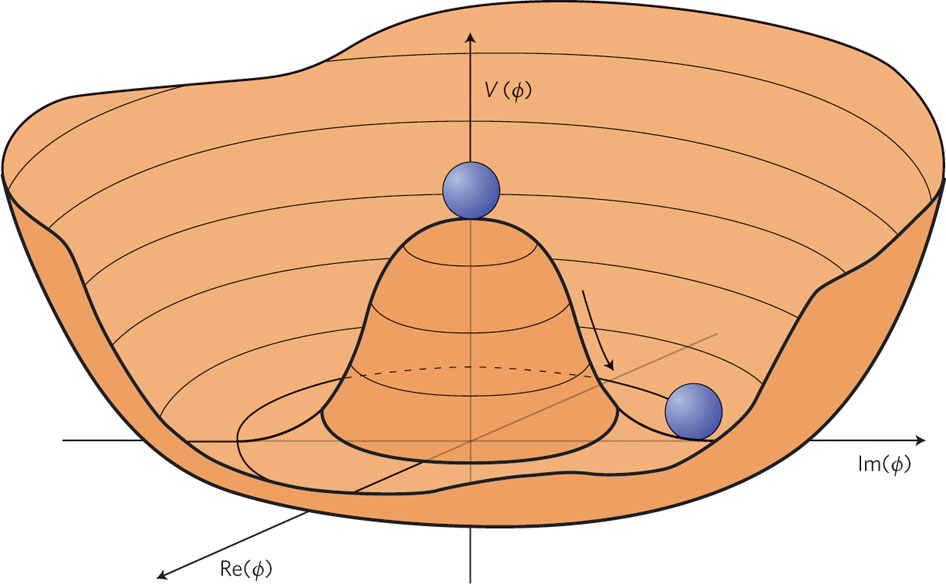
\includegraphics[width=0.6\textwidth]{Figures/Theory/MHat}
\caption[The Higgs potential chosen where $\mu^{2} < 0, \lambda > 0$ introducing degeneracy and breaking the electroweak symmetry into that of QED.]{\label{fig:MexicanHat}The Higgs potential chosen where $\mu^{2} < 0, \lambda > 0$ such that the minimum does not exist at 0, but instead in a ring of infinite minima about zero, thus introducing degeneracy and breaking the electroweak symmetry into that of QED.~\cite{MexHat}}
\end{figure}

The distinction between the two forces caused by this symmetry breaking are due to a linear combination of the weak hyper charge and isospin, $T_{3}$ and Y that vanishes for the Higgs. As this defines the conserved quantity Q for the electromagnetic group, this is not affected by the Higgs, and thus the $U(1)_{em}$ group remains unbroken. Conversely, the weak portion interacts with the Higgs and the W$\pm$ and Z bosons acquire mass.  

\section{Motivation for Physics Beyond the Standard Model}
The standard model has been widely successful, predicting the existence of particles such as the $W^{\pm}$ and Z Bosons, and the t quark, showing impressive agreement with experimental findings at the level of 0.1\%. However, there are several signs that it is not a complete theory, and that more information is needed to describe physics at higher energy scales. On the theoretical side, it is dissatisfying that the SM does not currently incorporate the gravitational force, explain the existence of dark matter and dark energy. Neutrino masses and flavour mixing are also unexplained, and the Higgs is as yet undiscovered. In addition it requires several input parameters to tune the masses of particles and flavour mixing, generally viewed as inelegant as this reliance on experimental data does not reflect the fundamental picture of nature.  The existing SM is therefore generally thought of as an effective theory, a very low energy approximation to a more complete theory\cite{PeskinSch}.

The incorporation of the gravitational force has not bothered particle physicists much at the electro-weak energy scale as the strength of the effects of gravity on fundamental particles is negligible compared to the other fundamental forces. However, at an energy known as the Plank Scale, $M_{p} \sim 10^{18}$ GeV quantum gravitational effects become important, leading to the breakdown of the existing QFT picture of the Standard Model. Thus new physics must exist at this energy scale, or before, indicating the SM is only valid up to some unknown energy scale. We think of the SM as a low-energy approximation of some larger more fundamental theory. In the event that no new physics exists prior to the Plank scale, the Higgs mechanism theory requires fine-tuning to lower the Higgs mass, which is considered to be ``unnatural". This is known as the ``hierarchy problem".

As there are both theoretical and experimental concerns over the SM, this provokes theories Beyond the Standard Model (BSM), many of which come in to play at the TeV scale, which we are able to explore for the first time with the LHC. A detailed description of a few of the most interesting shortcomings most relevant to this thesis are given below.

\subsection{The Hierarchy Problem}
Although the Higgs Boson has yet to be observed experimentally, its mechanism is necessary to the Standard Model to provide mass to the particles, and thus is considered to exist unless proven otherwise. However, while it solves the spontaneous symmetry breaking problem, the Higgs theory introduces theoretical issues of its own. The presence of the Higgs in the SM ensures the WW scattering amplitude does not violate unitarity, but only whilst the $m_{H} < 1$ $\textrm{TeV}$, providing an upper bound on the expected mass~\cite{WWHMass}. 

However, the mass of the Higgs, given by its self interaction receives extremely large radiative corrections. This is due to the heavy fermion anti-fermion pair loop contribution, seen in Figure \ref{fig:hiloop}. 

\begin{figure}
\centering
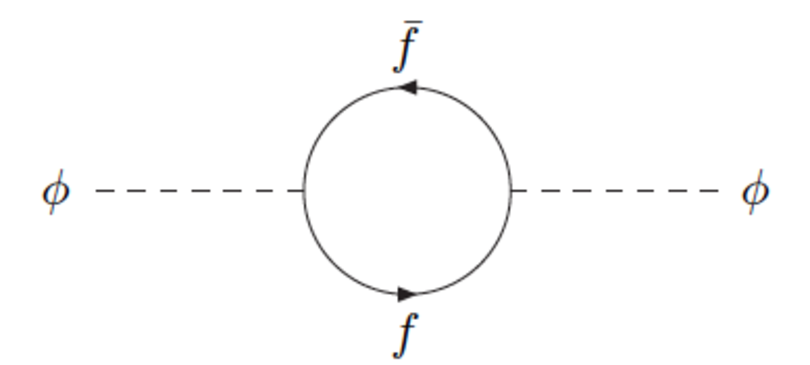
\includegraphics[width=0.4\textwidth]{Figures/Theory/higgsself}
\caption{\label{fig:hiloop}The loop contribution to the Higgs self-mass interaction from fermion-anti-fermion pairs in the SM}
\end{figure}

If each coupling with a fermion f has a term in the Lagrangian $-\lambda_{F} H \bar{f}f$, it contributes a quadratically divergent factor $\delta m^{2}_{H}$ that corrects the squared mass of the Higgs. 

\begin{equation}
\delta m^{2}_{H} =\sum_{f} - \frac{|\lambda_{f}|^{2}}{8 \pi^{2}}\Lambda^{2}_{UV} + \mathcal{O}(ln\Lambda)
\label{eqn:HIGGQUAD}
\end{equation}

The factor $\lambda_{f}$  represents the coupling for each type of fermion, which is largest in the case of the top quark, where $\lambda_{t} \approx. 1$. The parameter $\Lambda_{UV}$ is the \textit{ultraviolet cutoff}, so named as it represents the smallest distance probed in the calculation. It can be thought of as the scale up to which the Standard Model is valid, as any new physics would change the theory.

 If there were no new physics at a lower energy, it takes the value of the Plank Scale $M_{P}$, but in this case the correction will be 30 orders of magnitude higher than the 1 TeV upper bound justified experimentally\cite{Drees}. As there exists nothing in the SM to fix the Higgs Mass, the theory requires fine-tuning, tweaking the parameters to agree with observational findings. This is generally accepted to be an inelegant method, as it requires the input of extra information, and indicates a gap in the fundamental description leading to searches for extensions to the Standard Model. 

\subsection{Cold Dark Matter}

The existence of Dark Matter was postulated as early as 1933 by Zwicky \cite{zwicky}, as the orbital velocities of galaxies in clusters were inconsistent with their observed mass, suggesting some additional mass was present but not luminous.  Measurements of rotation curves of galaxies, cosmic microwave background and structure formation have confirmed this concept over the years. Experimental results from WMAP conclude only $\sim 4.5\%$ of the energy in our universe is made of the baryonic matter we see, while dark matter accounts for $\sim 23\%$ and the rest is comprised of another unknown, dark energy~\cite{WMAP5}. Although the existence of such matter has been well documented, there is still no understanding of the physics behind the phenomena. In order to explain the properties a weakly interacting massive particle (WIMP) is required, and it must be electrically neutral. There is no provisions for such a particle in the SM, indicating additional particle content requiring extensions in the theory. 

\subsection{Unification of Coupling Constants}

At the basis of theoretical particle physics is the observation of the symmetry and simplicity of nature. Unification, where several theories can be combined into one description,  has undergone before, first Electricity and magnetism, and then electromagnetism with the weak force. While each of the three forces of the SM have their own coupling constant, as the energy scale is increased the coupling constants converge towards one another. However precision measurements show that within the current framework,  there is no common point where all three intersect. In addition, at the Planck Scale as gravity's coupling constant would be of similar strength many hope for a Grand Unified Theory (GUT),  occurring at this scale known also as the GUT scale. This is only possible with the incorporation of some new physics which would alter the trend of the couplings between the electroweak scale and this GUT scale. 



\section{Supersymmetry}

Having discussed these major issues with the SM Theory, we move on to a discussion on a potential extension to the SM. There are several options, but this thesis will focus on the theory with what many consider the best solution to the three issues highlighted discussed in detail, beginning with a natural way to eradicate the hierarchy problem simply and without fine tuning.

The hierarchy problem could be removed, rather than controlled, if there were a way to cancel out the quadratic diverging term in the Higgs mass correction. As the correction for bosons has the opposite sign, the concept of a new symmetry was born, one between fermions and bosons. Known as SUperSYmmetry (SUSY), this theory extends the SM under this symmetry such that elementary particles in the SM each have a super partner differing by one half unit of spin as yet undiscovered, just as the anti-particles were once postulated. For every fermion contributing to the quadratic divergence, a boson partner contributes an equal and opposite term, and thus the hierarchy problem cancels out and the mass of the Higgs can take a sensible value.

Under this symmetry elementary particles in the SM would each have corresponding super-partners, differing by one half unit of spin, such that a fermion has a scalar boson super partner, and vice versa. At the heart of supersymmetry is a transformation that changes the field of a fermion into that of a boson, and vice versa. The generator of the transformation shall be known as Q,

\begin{equation}
\textrm{Q}|\textrm{fermion}\rangle = |\textrm{boson}\rangle,  \; \; \; \;  \textrm{Q}|\textrm{boson}\rangle = |\textrm{fermion}\rangle  
\label{eqn:Q}
\end{equation}

where the complex spinors that generate SUSY anti-commutate, with the following relationships where $P^{\mu}$ is the generator of space-time translations and indices are surpressed:


\begin{equation}
\{Q,Q\} = \{Q^{\dagger},Q^{\dagger}\} = 0 \qquad \{Q,Q^{\dagger}\} = P^{\mu} 
\end{equation} 



In addition to its neat solution to the hierarchy problem SUSY has several other consequences which lead to its position as a favoured theory for new physics at the TeV scale. The addition of SUSY particles to the SM has the side affect of altering the runnings of the gauge coupling constants of the three fundamental forces. Figure \ref{fig:couple} shows the running constants from the SM alongside those with the SUSY model incorporated. Whilst the SM allowed only two to intersect at any point, SUSY alters them such that they are consistent with theories of Grand Unification, as the three are equal at the GUT scale Q $\sim 10^{16}$ GeV. 

Rather than a motivation, this is a pleasant coincidence, but lends plausibility to the theory. It also shows promising features necessary for theories to incorporate gravity, although it does not finish the job. SUSY itself cannot be the final fundamental theory of particle physics, but is an extension which shows much promise, and is a pre-requisite for many higher energy theories such as most formulations of String Theory\cite{Dine}. The final, perhaps most exciting feature of SUSY is that it can offer a candidate for the particle that represents dark matter with the introduction of a new quantum number R - Parity. 

\begin{figure}
\centering
\subfigure{\label{snk}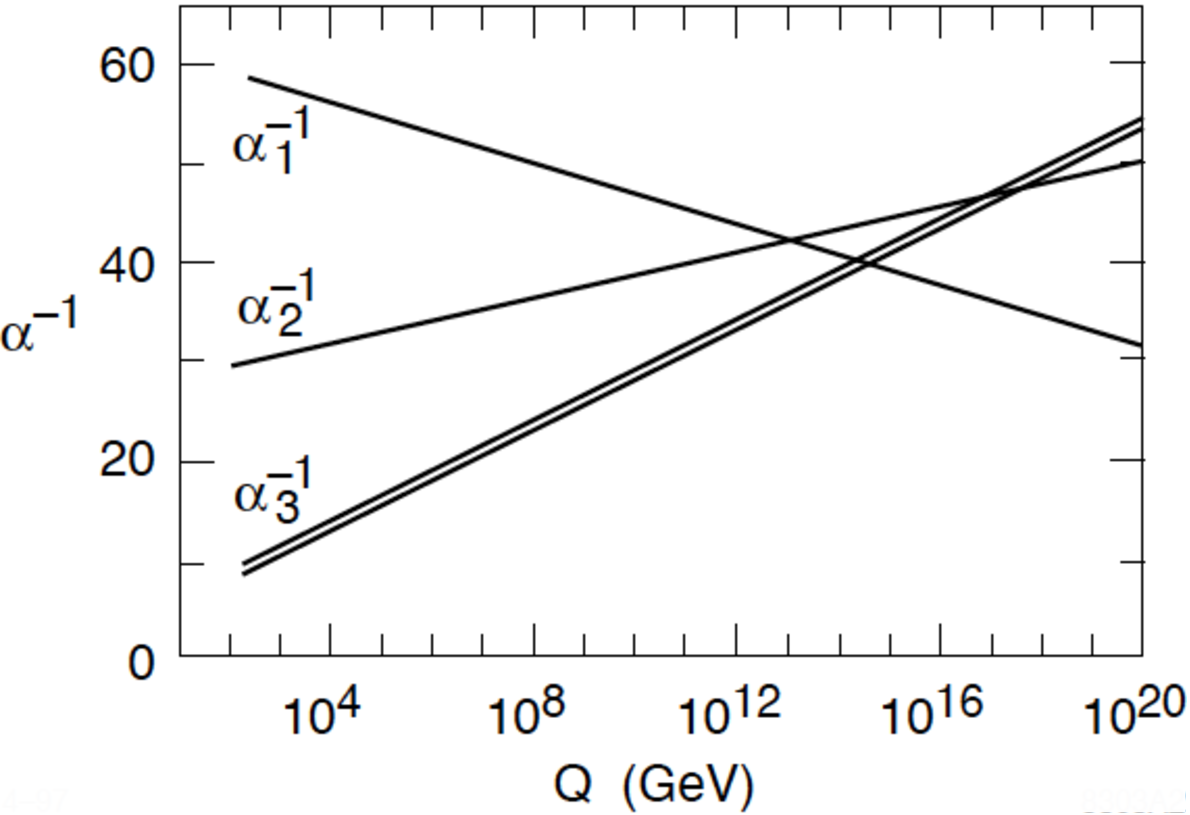
\includegraphics[width=0.40\textwidth]{Figures/Theory/smcoupling}}
\subfigure{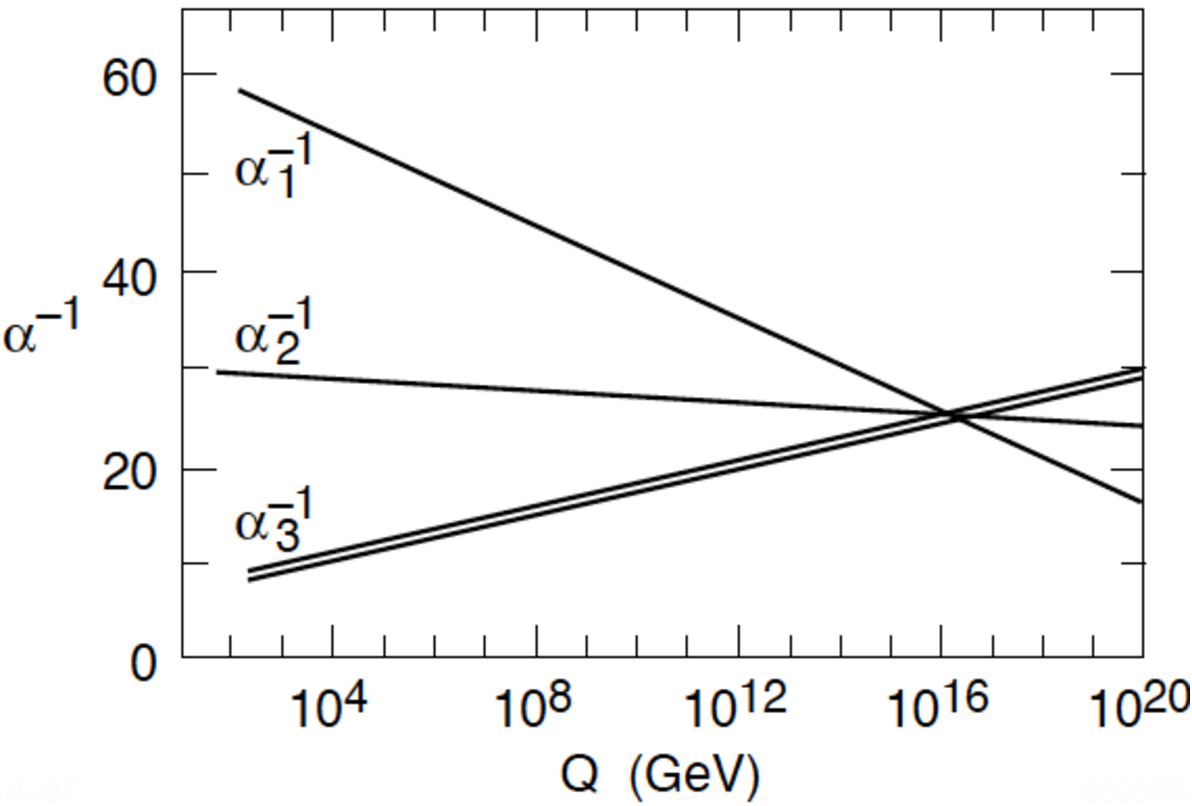
\includegraphics[width=0.40\textwidth]{Figures/Theory/susycoupling}}
\caption[The running gauge coupling constants for $SU(3)_{C} \times SU(2)_{L} \times U(1)_{Y}$ in the SM and SUSY cases.]{\label{fig:couple}(a) The SM running gauge coupling constants for $SU(3)_{C} \times SU(2)_{L} \times U(1)_{Y}$ are shown with increasing energy scale Q. (b)same plot is made after the supersymmetric extension to the Standard Model has been applied. The double lines for $\alpha_{3}$ indicate the error in experimental  measurement, which is negligible for the other two.~\cite{PeskinBSM}}
\end{figure}



\subsection{R-Parity}

Constructing the most general form of SUSY, terms appear which allow processes which violate two quantum numbers, the baryon number B and the lepton number L. Whilst there is no theoretical reason for this to be a problem, these interactions have not been observed, and are constrained heavily. An undeniable constraint is the lifetime of the proton, which is very large, whereas these processes would facilitate its decay. whilst B and L are not fundamental symmetries in the theory, it is possible to construct a new quantum number R defined in Equation \ref{eqn:RPAR} which can be required as a symmetry R-parity\cite{terning}. It distinguishes between particles from the SM and the sparticles introduced by SUSY, as under this construction, all SM particles carry $R$ of +1 and all super partners carry -1. 

\begin{equation}
R = (-1)^{3(B-L)+2S}
\label{eqn:RPAR}
\end{equation}
Whilst terms in the Quantum Field Theory do allow for the possibility of violation of this parity, experimental measurements have excluded this for sparticles with masses on the TeV scale, and therefore those within the reach of the LHC. Thus the  majority of searches consider models with a symmetry which forbids this violation and conserves Rp. Several phenomenological consequences that transcend specific models arise from this assumption which provide the backbone to SUSY searches at the LHC:

\begin{itemize}
\item{In order for SUSY particles to be produced at the LHC under this framework, they must be pair produced from SM particles.} 

\item{The heavier particles will cascade down a decay chain ending through creation of the lightest of the supersymmetric particles, denoted the Lightest Super Partner (LSP)}

\item{The LSP must be stable as it cannot decay into SM particles, and through cosmological bounds must be electrically neutral.} 
\end{itemize}
These characteristics of the LSP show us that it is a WIMP, the type of particle that is sought in Dark Matter searches.  These particles will not interact in a detector, therefore are characterised in an experiment as large amounts of missing energy. As this is directly a characteristic of a WIMP in the final state, such a signature represents not only SUSY but is shared by other new physics models with a dark matter candidate particle. 

Models may be constructed to constrain the violation of B and L without R-parity conservation, but those shall not be considered in this thesis, as this unique feature provides both physical motivation and a search strategy for physics at the LHC.


\subsection{MSSM} 

Whilst there are many ways to construct mathematically the theory of Supersymmetry, it is usual to do so in a way which introduces the least number of new degrees of freedom. This demands the minimal particle contact required to satisfy the core symmetry, which corresponds to one new degree of freedom for each existing SM one. This approach is known as the Minimal Supersymmetric Standard Model (MSSM), and has an additional new particles, known as a sparticle, for each known SM particle. 

The particles are arranged to fit the irreducible representation of the symmetry, in \textit{supermultiplets}, each of which contains both fermions and bosons. The number of bosonic and fermionic degrees of freedom are therefore equal in any supermultiplet. There are two types of supermultiplet available, a chiral supermultiplet which describes a left-handed fermion, its right handed anti-particle, a complex boson and its conjugate, and a vector multiplet - a massless vector field and a left handed fermion, which result in the fermion and its anti-particle and two transversely polarised vectors bosons\cite{SUSYPrime}. 

The names of the spin-0 bosons that partner the SM fermions are prefixed with ``s-", known as squarks and sleptons, collectively the sfermions. As the SM contains a distinction between left and right handed fermions, the boson super partners have one of each too, and are labelled RH and LH, but it is important to remember this is not a description of the super partner itself, merely a label to describe the SM particle is associated with. The particles are written with a tilde above the SM symbol so the top quark t becomes the "stop" quark, $\tilde{s}$.

The names of the fermions from the SM bosons are appended with ``-ino" such as the super partners of the gluons, the gluinos. However, for the other fundamental SM bosons, identifying their super-partners is not so simple. The symmetry acts not on the results of electroweak symmetry breaking but on the fields of the $SU(2)_{L} \times U(1)_{Y}$ group. Thus there should be three Winos \~{W} and a Bino \~{B}. 

The Higgs receives different treatment in SUSY than that discussed earlier for the SM, where the scalar field gives up three degrees of freedom to give mass to the vector bosons W$^{\pm}$ and Z. In SUSY, instead two supermultiplets with differing quantum number are required to maintain the electroweak symmetry breaking, one chiral and one vector. These give mass respectively to the up-type quarks of charge $-\sfrac{1}{3}$ and the down-type quarks of charge$+\sfrac{2}{3}$, and thus are named $H_{u}$ and $H_{d}$\cite{SUSYsuch}. Where the SM has one complex doublet, the MSSM has two complex Higgs doublets, hence the sector has 8 degrees of freedom. Three are lost to give the W$^{\pm}$ and Z bosons mass in electroweak symmetry breaking, leaving five which represent five Higgs boson particles: the charged Higgs bosons $H^{\pm}$, and three neutral bosons h, H and A. The corresponding super-parters are known as the higgsinos.  


\subsection{Supersymmetry Breaking}

In order to satisfy an exact symmetry, one would expect that each super-partner would have the same characteristics as its SM partner, including its mass. This would indicate they were within the reach of previous physics experiments, but it is clear this is not true as there has been no experimental evidence of particles in the energy spectra previously covered by experimental research. Drawing parallels with the problem of electro-weak symmetry breaking, we say SUSY is broken by some mechanism, resulting in particles with heavier masses than their counterparts. Although the size of these masses could be theoretically anything, in order for SUSY to eliminate the hierarchy problem this breaking must occur at the Electroweak Scale, which puts an upper bound on the mass differences of around 1 TeV.  

This is known as ``soft" SUSY breaking, and offers the hope of discovering this new physics at the TeV scale, as is now possible for the first time with the LHC. This involves ``soft" mass terms incorporated into the Lagrangian theory that do not introduce quadratic divergences that would provide a new "hierarchy problem". However, the nature of this breaking is not known and thus it is traditional to formulate it in the theory to contain all the mass and mixing terms allowed by the underlying symmetry, which gives arbitrary masses to the sparticles. As there are many unknowns this introduces a large number of parameters to the system. Not all is lost, as SUSY is still capable of making useful predictions, however to compete the theory an understanding of the nature of SUSY breaking is really required. 

Due to electroweak symmetry and soft SUSY breaking the fermions super-partners of the $SU(2)_{L} \times U(1)_{Y}$ group are not generally the mass eigenstates. Instead the winos and bino mix with the higgsino fields to produce the mass eigenstates in two groups, the charginos $\tilde{\chi}^{\pm}_{1,2}$ and the neutralinos $\tilde{\chi}^{0}_{1,2,3,4}$


\subsection{Minimal Supergravity and the Constrained MSSM}

Even assuming a minimal particle content, the MSSM has a large number of free parameters, introduced through SUSY and Electroweak symmetry breaking, 105 new parameters in addition to the 19 already present in the SM. When it comes to experimental searches, this is an unworkable number, for to examine possible behaviour of SUSY one would have to look in 105 dimensions. Thus for the purpose of making models to work with, it is desired to constrain this number of free parameters in the theory. One popular GUT model is the theory of minimal SUper GRAvity, otherwise known as mSUGRA. 

The many parameters of the MSSM are in fact not all constants, but rather vary with the energy scale. Thus, to contain the model the we can assume that there is some ``hidden sector" (perhaps on the order of the $M_{P}$) which contains fields with no couplings to what is now thought of as the ``visible sector" of the MSSM. There should then be some messenger between the two, that allows supersymmetry breaking to be mediated by the MSSM in order to provide the soft terms. One popular theory as to the nature of this messenger is that it is ``gravity mediated". 

The MSSM combined with the theory of mSUGRA is called the Constrained MSSM, or CMSSM, as the number of free parameters is reduced to a manageable five. These factors are:

\begin{itemize}
\item{A common scalar mass $m_{0}$}
\item{A common gaugino mass $m_{1/2}$}
\item{The SUSY Breaking common trilinear coupling $A_{0}$}
\item{The ratio of the vacuum expectation values of the two Higgs Fields tan $\beta$}
\item{ The sign of the Higgs parameter, sign($\mu$)}
\end{itemize} 

With this relatively small parameter space it is possible to construct models with which to construct search strategies, and allows us the exclusion of regions with the advent of new results. A given point in mSUGRA space defines the mass hierarchy of the squarks, gluinos, charginos and neutralinos, therefore governing the interactions that are possible, as well as the identity of the LSP. Thus in different regions the productions mechanisms can differ, however in the majority of phase space the LSP is the lightest of the neutralinos, $\tilde{\chi}^{0}_{1}$.  For convenience, mSUGRA is shown graphically in the $m_{0}$ - $m_{1/2}$ plane, for set values of the other three parameters. 

There are other theories that support mechanisms of SUSY breaking, such as Gauge-Mediated Symmetry Breaking (GMSB) and Anomaly Mediated Symmetry Breaking (AMSB) but these are not considered for the purpose of this thesis. 

\subsubsection{Current Limits on the CMSSM}

Two types of limits exist in mSUGRA space, those imposed theoretically and those that result from experimental data. Of the latter, some are contributed by cosmology, and others by particle physics. 

There are some regions of the parameter space where the masses of the particles have a hierarchy which results in the stau being the LSP. This is theoretically forbidden as the LSP certainly contributes some if not all of the dark matter in the universe, and it is known to be neutral. 

In addition, a further region is excluded whereby the relic density of the LSP is consistent with the WMAP measurement of the Dark Matter density. 

\subsection{Production Mechanisms in pp collisions}
At a proton-proton collider at TeV energies such as the LHC, as discussed before we can consider the protons as a set of partons each carrying a fraction of the total momentum. It is these quarks and gluons that collide. At such high energies these can be from the gluons in the sea as well as the valence quarks, thus there are qq, $q\bar{q}$, qg and gg collisions to consider.
Assuming SUSY exists within the reach of the LHC, indicated by the restriction imposed on the mass differences of SUSY breaking, then from these interacting pairs large production rates of both squarks and gluinos are expected. Cross sections in the region of 100 pb to 1fb are possible for SUSY sparticles with masses between 0.5 TeV and 1 TeV~\cite{early}. Predominantly the production is the result of strong processes resulting in squarks and gluinos, although weak production is predicted albeit at smaller cross sections. Decays from these particles through charginos and neutralinos would result in production of the LSP, but the structure of these decays depends on the mass hierarchy of the sparticles, which is determined by the values of m$_{0}$ and m$_{1/2}$.  Thus a chosen point in this plane represents a certain set of kinematics. SUSY production in these collisions is dominated by the pair-productions $ qq \rightarrow \tilde{g} \tilde{g}, \tilde{q}\tilde{g}, \tilde{q} \tilde{q}$. The relative cross sections of these decay modes depend on the region of mSUGRA 

\begin{figure}
\centering
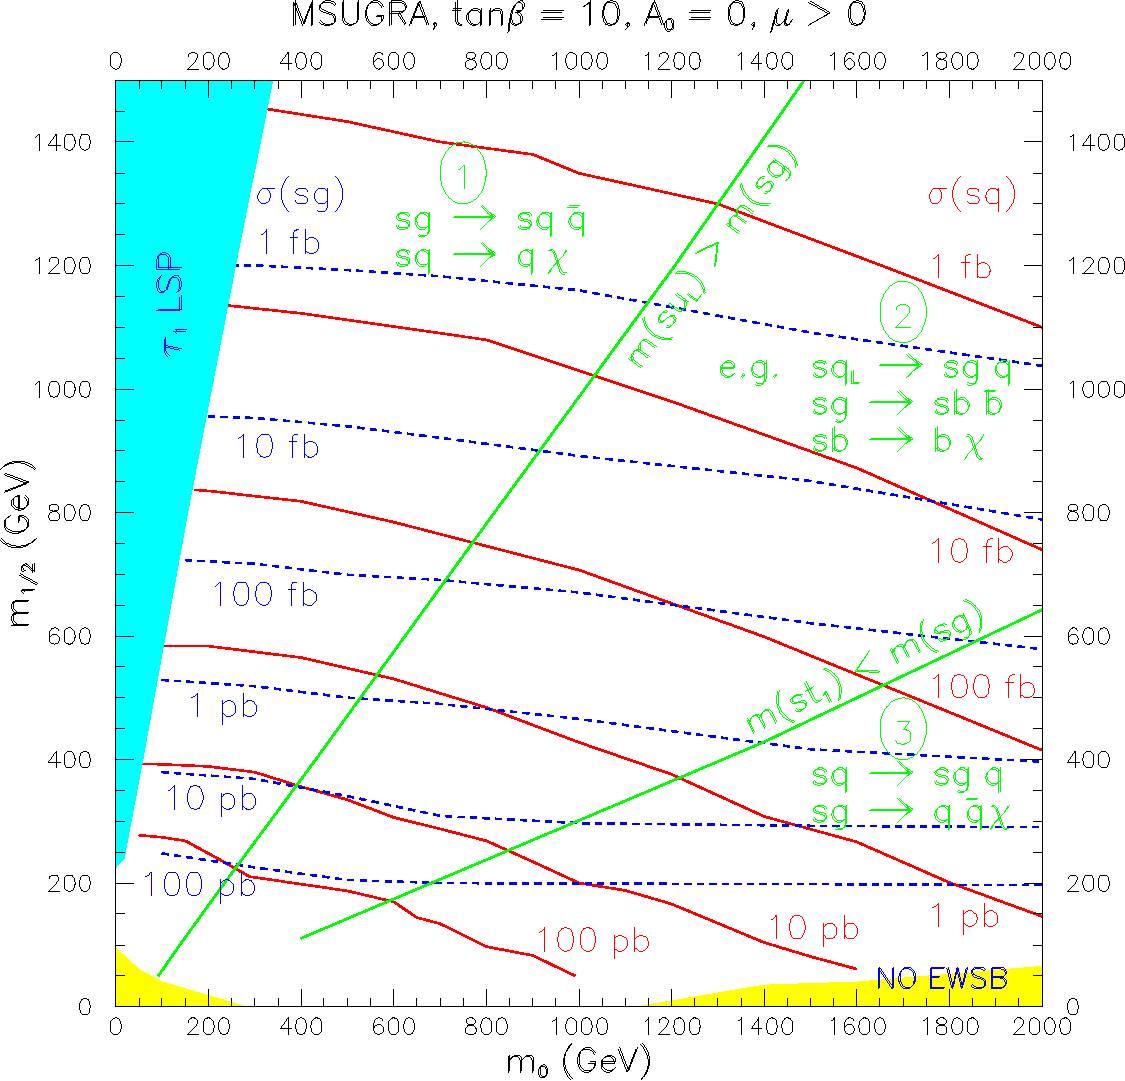
\includegraphics[width=0.6\textwidth]{Figures/Theory/mSUGRA_TDR_1}
\caption[The $m_{0}-m_{1/2}$ plane of mSUGRA depicting diagonal lines separating three distinct regions of mass hierarchies based on the mass difference of squarks and gluinos. ]{\label{fig:msugratdr}The $m_{0}-m_{1/2}$ plane of mSUGRA depicting diagonal lines separating three distinct regions of mass hierarchies based on the mass difference of squarks and gluinos. Lines of constant production cross section for squarks and gluinos are shown in red and blue respectively. The allowed decays in each region are shown, where ``sq" denotes a squark, and ``sg" a gluino.\cite{CMSTDRII}}

\end{figure}

Within mSUGRA there are three distinct regions which exhibit different decay modes, defined by the mass relationship between the gluinos and the squarks. These an be seen Figure \ref{fig:msugratdr} , where the diagonal green lines represent a cross-over in the squark-gluino hierarchy. Passing left-right on the diagram, the regions are:

\begin{description}
\item[Region1: $m_{\tilde{g}} > m_{\tilde{q}}$]{As the gluinos are heavier than the squarks, the general form of decays is
\begin{equation}
\tilde{g} \rightarrow \tilde{q} \bar{q} , \tilde{q} \rightarrow q \chi
\end{equation}
}
\item[Region 2: $m_{\tilde{g}}< m_{\tilde{q}_{L}}, m_{\tilde{g}}> m_{\tilde{t}_{1}} $]{Here the mass of the gluino between that of the heaviest and lightest squark, therefore more complicated decay relationships between the two are allowed, and these depend on exactly which quarks are heavier and which lighter. The $\tilde{q}_{L}$ are the heaviest, while states such at $\tilde{b}_{1}$ and $\tilde{t}_{1}$ are some of the lightest. The heavier quarks decay to lighter squarks and to gluinos, and the gluino decays to lighter squarks. }
\item[Region 3: $m_{\tilde{g}} < m_{\tilde{q}}$]{Finally in this region the gluino is lighter than any squark, and the allowed decays take the form
\begin{equation}
\tilde{q} \rightarrow \tilde{g}q , \tilde{g} \rightarrow q\bar{q} \chi
\end{equation}
}
\end{description}

As the dominating decay of both squarks and gluinos produce quarks, we expect in a SUSY event many hadronic jets from these sources along with the gluon radiation from the incoming and outgoing partons. Thus a traditional SUSY signature that provides the basis for this thesis is that of multiple jets and evidence of a (missing) LSP. 




%\chapter{The Compact Muon Solenoid Experiment at the LHC}
\label{ch:detector}

Throughout history knowledge has been advanced through a combination of theoretical postulation using mathematical tools, and experimental searches. The theoretical formulation of particle physics is complimented by experimental searches that confirm or deny expectations. The exploration is furthered by delving into smaller and smaller distance scales using particle colliders with greater energies, and analysing the interactions that result. This relationship between small distances and high energies is at the heart of the field, as each increase of energy scale allows the investigation of the structure of matter at a smaller length scale. In the current era the TeV scale is accessible at experiments for the first time, leading to investigations into the validity of the Standard Model at this energy and attempts to observe new physics beyond. 

\section{The Large Hadron Collider}

The Large Hadron Collider (LHC) is a double-ring circular synchrotron at CERN designed to collide two proton beams with a centre of mass energy $\sqrt{s}$  = 14 $\tev$ at a final design luminosity of $10^{34}$cm$^{-2}$s$^{-1}$. The energy and luminosity have been chosen with the aim of discovering new physics at the TeV scale, beyond the reach of previous experiments, where theories predict physics both within and outside the Standard Model. It will also be used to collide heavy lead ions (Pb$^{82+}$) to an energy of 2.76 $\tev$  per nucleon, in specific runs, with the purpose of investigating QCD matter at energies 30 times higher than previous experiments. 
The LHC has unparalleled reach in the search for new physics, not only due to the significant increase in energy over the Tevatron, the previous record holder, but also due to the intensity of the beams delivered. The number of events, $n$, produced by a given physical process depends on its cross section $\sigma$, which is proportional to $\sqrt{s}$, and the luminosity $\lumi$, which has the dependence shown in Equation \ref{eq:lumi}~\cite{LHCDesign},

\begin{equation}
n = \lumi \sigma, \hspace{.75in} \lumi = \frac{N_{b}^{2} n_{b} f_{rev} \gamma_{r}}{4 \pi \epsilon_{n} \beta^{*}}F,
\label{eq:lumi}
\end{equation}

where $N_{b}$ is the number of particles in a single bunch, $n_{b}$ is the number of bunches in a beam, $f_{rev}$ the frequency of revolutions, $\gamma_{r}$ is the relativistic gamma, $\epsilon_{n}$ is the beam emittance and $\beta^{*}$ is the value of the amplitude function associated with the collision point. The geometric luminosity function, $F$, provides a reduction factor based on the beam crossing angle, and depends on the full crossing angle at the point of interaction $\theta_{c}$, and the transverse and longitudinal RMS beam dimensions $\sigma_{*}$ and $\sigma_{z}$ with the following dependency:
\begin{equation}
F^{2} = \frac{1}{1+(\frac{\theta_{c} \sigma_{z}}{2\sigma_{*}})}
\label{eq:lumi2}
\end{equation}

Situated in the tunnel of the previous $e^{+}e^{-}$ machine LEP located underneath the Franco-Swiss border,  the LHC is mostly circular with a circumference of 27km, consisting of 8 arced sectors connected by 8 straight sections in which are the numbered Interaction Points (IP), where the two beams circulating in opposite directions can be made to collide. To bend the protons around the rings, the two beams experience opposite dipole fields from one another, and have two separate vacuum systems. As the tunnel has restricted space available, the dipole magnets are twin bore with two coils and share the same structure and cryogenics. The 1232 superconducting dipole magnets present must produce a field in excess of 8T due to the high momentum of the protons, and thus have a high current and must be cooled below 2K by liquid helium to ensure safe operation. The beams are non-continuous, grouped in ``bunches" at intervals. In the straight sections the two beams share the same beam line and can be directed to coincide at the IP's. In order to maximise the number of interactions, quadrupole magnets are used to focus the beam providing a minimum cross section at the point of interaction.

The four main detectors that analyse the data from collisions are located at four of these IPs: the two high luminosity experiments ATLAS\,(A Toroidal LHC Apparatus) at IP1 and CMS\,(Compact Muon Solenoid) at IP5 are multi-purpose detectors analysing the p-p collisions for signs of new physics. At IP8 the LHCb\,(LHC beauty) detector looks for CP violation and other rare decays in a forward detector with lower luminosity runs, and ALICE\,(A Large Ion Collider Experiment) at IP2 will investigate the lead-lead ion collisions. The locations of the detectors in the LHC ring is shown in Figure \ref{fig:LHC}~\cite{LHCConcept} .

\begin{figure}[htbp]
\centering
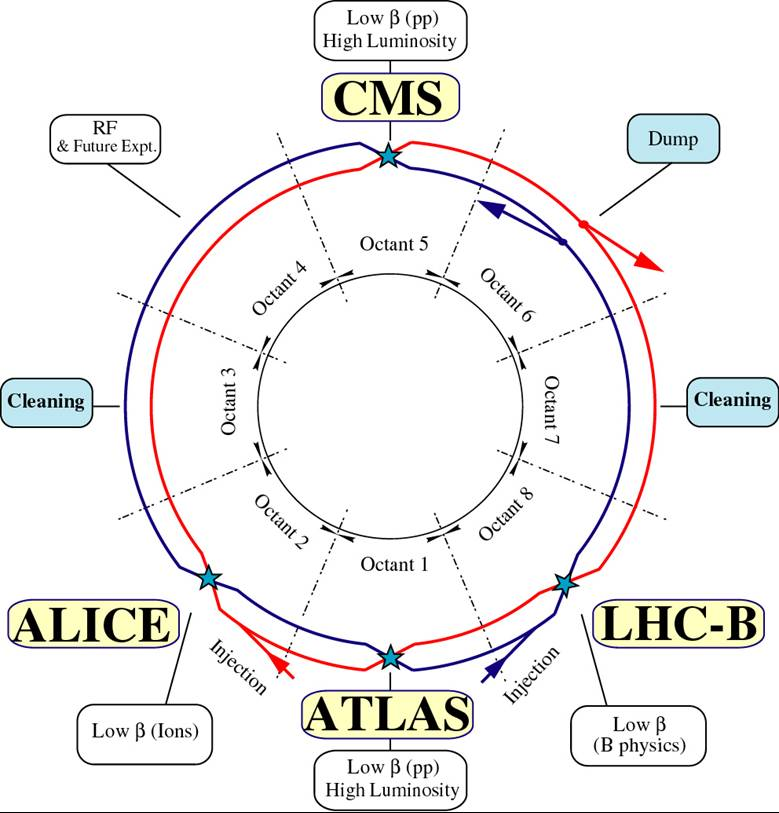
\includegraphics[width=0.85\textwidth]{Figures/Detector/lhc-schematic}
\caption[Schematic of the LHC ring and the location of the major experiments.]{Schematic of the LHC ring and the location of the major experiments~\cite{LHCConcept}.}
\label{fig:LHC}
\end{figure}


The magnets are optimised for beams of a certain energy range, and therefore the protons cannot be fully accelerated in the LHC. Therefore the supply of protons are delivered through a series of other machines that make up part of the CERN accelerator complex, the layout of which is shown in Figure \ref{fig:LHCinject}. 

A beam of 50\,MeV protons is created in LINAC2, in 6 bunches, and each bunch is then split into 12, resulting in 72 bunches which are fed into the Proton Synchrotron Booster. After accelerating to an energy of 1.4~GeV, they enter the Proton Synchrotron, where they are accelerated to 26~GeV. Then 2-4 sets of 72 bunches are fed into the Super Proton Synchrotron. Now 144-288 bunches, they are accelerated to 450~GeV ready for injection into the LHC. Twelve of these sets are injected into the LHC, directly into both rings, giving a nominal bunch density of 2808, with a spacing of 25\,ns. This process takes around 20 minutes, and then the LHC takes a further 20 minutes to ramp the protons up to the desired energy by raising the current of the dipoles. The magnets preventing the beams coinciding in the detectors are turned off and stable collisions occur. The luminosity falls regularly as the run progresses as protons are lost in collisions, and after 6-12 hours, it has fallen below an acceptable level, and the beam is dumped before repeating the process again. 

Using these short runs of high luminosity it is possible for the LHC to take large amounts of data, and assuming 200 days of data taking a year  at design luminosity the machine will be able to deliver 100~fb$^{-1}$ a year. As part of the early phase of operation the machine was operated in 2010-2011 at 3.5~TeV per beam, $\sqrt{s} = $7~TeV, in order to protect the magnets, and is not expected to run at full energy until 2014. The 2011 run delivered 5.727~fb$^{-1}$ data, the first 1.1~fb$^{-1}$ of which was delivered by the end of June, and is considered for this thesis.

\begin{figure}[htbp]
\centering
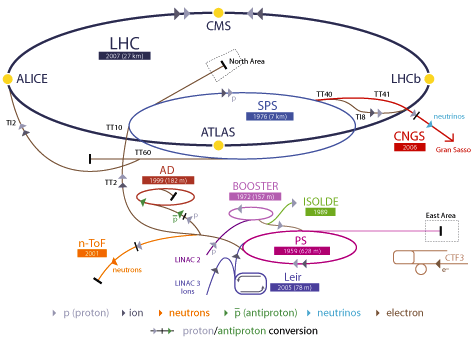
\includegraphics[width=0.8\textwidth]{Figures/Detector/injection}
\caption[Layout of the CERN accelerator complex, illustrating the relationship between the LHC and its supporting accelerators tasked with delivering proton beams at 450~GeV.]{Layout of the CERN accelerator complex, illustrating the relationship between the LHC and its supporting accelerators tasked with delivering proton beams at 450~GeV~\cite{Christiane}.}
\label{fig:LHCinject}
\end{figure}



\section{The Compact Muon Solenoid}

The Compact Muon Solenoid (CMS) is one of the two high-luminosity multi-purpose detectors at the LHC, designed to capitalise on the full range of physics opportunities available as the new energy scale is probed. These goals are pursued through the design and construction of the detector and development of software for the reconstruction of physics objects. The detector is constructed of several detector sub-systems contained inside and wrapped in layers around a central 13\,m long 4\,T super conducting solenoid as shown in Figure \ref{fig:CMS_Struct}. 

The detector is 21\,m long, 15\,m wide, weighs 14000 tonnes and consists of five wheel-like barrel sections and two end-caps. In order for CMS to search for new physics among the high Standard Model backgrounds, it is of key importance to develop a detector which has excellent energy and momentum resolution resulting in accurate particle identification. Different particles interact differently with matter and therefore a number of different sub-detectors are needed in order to gather all the relative information. These data are then combined in order to reconstruct the objects. 

\begin{figure}[htbp]
\centering
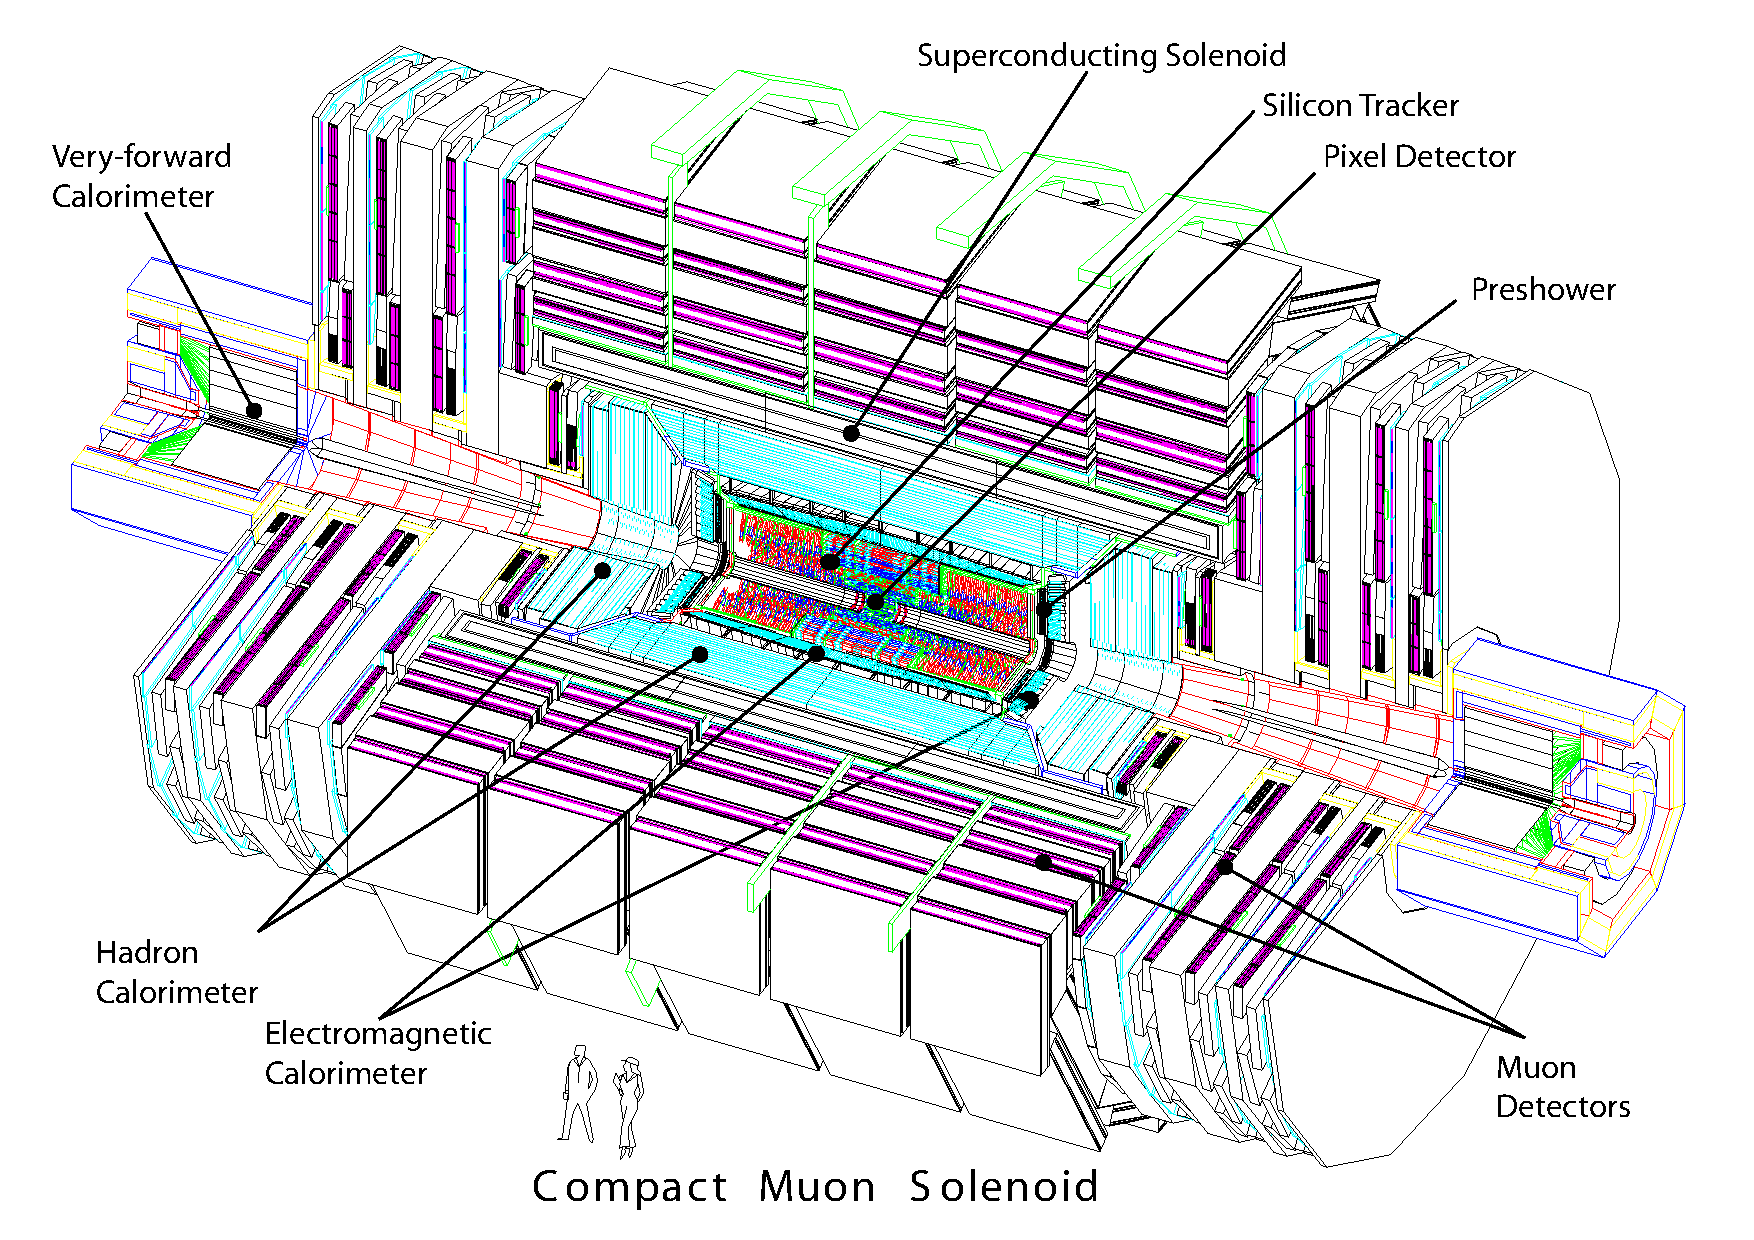
\includegraphics[width=0.9\textwidth]{Figures/Detector/CMS_Structure}
\caption[A cutaway diagram of the CMS detector structure identifying the main individual sub-systems.]{A cutaway diagram of the CMS detector structure identifying the main individual sub-systems~\cite{TDRVOLI}.}
\label{fig:CMS_Struct}
\end{figure}

The high magnetic field was chosen in order to achieve the bending power necessary for good charged particle momentum resolution. The inner bore of the solenoid is large enough that the inner tracker and the calorimeters are located inside, which minimises the material the particles pass through before entering the calorimeters. This improves the energy measurement resolution. Four muon ``stations" of aluminium drift tubes are integrated within the iron magnetic field return yoke. The full design description can be found in the CMS Technical Design Proposal \cite{CMSTDP}. As different particles pass through the detector they interact in the sub-systems depending on their type. A transverse slice through the detector illustrating the path through the machine of each type of particle is shown in Figure \ref{fig:CMS_Slice} 





\begin{sidewaysfigure}
\centering
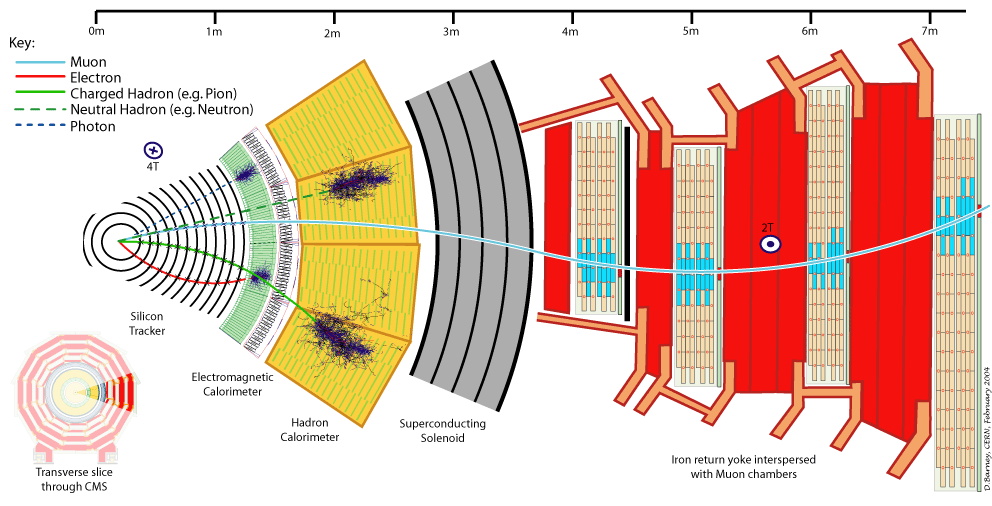
\includegraphics[width=1.\textwidth]{Figures/Detector/CMS_Slice}
\caption[Transverse slice through the CMS Detector showing the path of each type of particle and how it interacts with the sub-detectors.]{Transverse slice through the CMS Detector showing the path of each type of particle and how it interacts with the sub-detectors~\cite{cmsslice}.}
\label{fig:CMS_Slice}
\end{sidewaysfigure}
\subsection{Coordinate System}

The coordinate system chosen by CMS uses the nominal interaction point within the detector as the origin. The x-axis points radially inwards to the centre of the collider ring, and the y-axis points vertically upward. The z-axis then points in the direction of the anti-clockwise beam. The azimuthal angle $\phi$ is defined as the angle from the x-axis in the x-y plane, and the polar angle $\theta$ from the z-axis. However, it is common convention to express $\theta$ in terms of the quantity pseudorapidity,~\begin{math}
\eta = -\ln \tan (\theta / 2) 
\end{math}, as particle production is approximately uniform in $\eta$. The transverse components of the energy and momentum, denoted $E_{T}$ and $p_{T}$ are then calculated from the $x$ and $y$ components. 



\subsection{Superconducting Magnet}

The geometry of the magnetic field is integral to the design and cylindrical structure of the CMS detector, as it uses a global solenoidal magnet. A strong magnetic field is essential to the design of a detector, bending charged particles in order to measure their charge and momentum. In order to ensure that the curvature is significant even with particles of high momentum, the CMS solenoid is designed to be capable of delivering a homogenous field of 4\,T within its volume. Consisting of four layers of NbTi coils in a vacuum with a cryogenic system maintaining a temperature of 4.5\,K, the solenoid has a diameter of 5.9\,m and length 12.5\,m, and when operating at full current is cable of storing 2.6~GJ of potential energy.

As the solenoid is so large, not only the inner tracking system but also both calorimeter sub-detectors can be accommodated in the interior, giving significant advantage to electromagnetic and jet energy resolution as particles will not have traversed the high-density magnet coil before these measurements are taken. The flux is returned with a large iron yoke of $10^{7}$~kg, surrounding the inner magnet and built with a barrel of 5 wheels, and two end-caps each containing three disks. The muon system is built within the iron return yoke, in order to take advantage of the reverse magnetic field produced in the outer region, and thus follows the same structure. The drawback of a solenoidal field is that it has strong inhomogenity in the end-caps, affecting the performance of the muon subsystem, which shall be discussed later.


\subsection{Tracker}



The first sub-detector encountered by particles is the multi-layer silicon tracker, which records precise information about the path of charged particles bending under the magnetic field. The inner layers are placed as close to the interaction point as possible in order to distinguish the primary interaction from secondary vertices of particles with significant lifetimes. This is particularly important in the case of identifying B mesons, which can travel a measurable distance before decaying.  

The tracker is divided into regions defined by the radius, $r$, from the interaction point, as the expected particle flux decreases rapidly as the radius increases. This is due not just to the increase in area of the solid angle, but also to the high magnetic field, which causes low momentum particles to have small radial helical trajectories.

Nearest to the primary vertex at 4\,cm, where the expected particle flux is at its highest ($\sim10^{8}$\,cm$^{-2}$\,s$^{-1}$), is the pixel detector which consists of 66 million silicon pixels of size 100 $\times$150\,\textmu m$^{2}$ arranged in three barrel layers and two end-cap disks. This region is laid out to optimise the resolution in determining the vertex position, delivering a hit resolution of $\sim$10\,\textmu m in the $r-\theta$ plane and $\sim$ 20\,\textmu m in the $r - z$ plane. Pixel detectors have the advantage of being able to measure all three coordinates of the particle simultaneously. However this requires a large number of readout channels and drives the costs of construction up. For this reason pixel detectors are chosen for the innermost region where the flux is highest, while the rest of the detector is composed of silicon micro-strip devices. 

Outside of the pixel detector lies the silicon strip tracker with its first layer located at $r$ = 20\,cm. It is divided into two parts, the inner and outer components. As the flux of particles expected is lower than in the pixel detector, the use of 11.4 million silicon strips allows the desired granularity while minimising costs. Whilst these do not allow a simultaneous 3-coordinate measurement, some of the layers are constructed at known angles to the others and therefore when combined all three coordinates can be measured. The inner region, immediately outside the pixel tracker, is composed of four barrel layers (TIB) and closed with three disks (TID) on each end, occupying the region up to $r$~=~55\,cm, where the microstrip sensors are 320\,\textmu m thick oriented along the beam line in TIB and radially in the TID. The outer region has 6 barrel layers (TOB) further apart than in the inner sector, and closed with 9 end-caps (TEC) on the end of the barrel, extending out to $r$~=\,116\,cm. The strips here are 500\,\textmu m thick.

In total the tracker covers a total area of 205\,m$^{2}$ with 76 million channels and provides a transverse momentum measurement for high momentum tracks with resolution 1 - 2\,\% in the region $|\eta| <$ 1.6.

\subsection{ECAL}

Immediately outside of the tracker, and still within the magnet core, sits the Electromagnetic Calorimeter (ECAL), used to measure the energy of electrons, photons and pions via the energy they lose through radiation. Electrons lose their energy in the material through \textit{bremsstrahlung}, and photons by decaying to an electron-positron pair. Using a hermetic homogenous calorimeter of scintillating crystals, this energy can be converted to scintillation light which is picked up by a light sensitive detector. 

The use of high density crystals allows a fast calorimeter which has fine granularity and is radiation resistant, requirements which are essential in the LHC environment. After rigorous research and development, lead tungstate (PbWO$_{4}$) crystals were chosen as the optimal solution to the requirements of LHC operation, due to a number of desirable characteristics. The extremely short radiation length $X_{0}$ = 0.89\,cm allows the construction of a compact ECAL which therefore can reside within the solenoid, hence reducing the amount of material particles have to pass through before reaching the calorimeter. In addition, the material has a small Moliere radius (2.2cm) meaning the transverse size of the electromagnetic shower is narrow, leading to good shower position resolution and separation. It is also essential that a fast scintillator is used, in order to distinguish between bunch crossings. In crystals of PbWO$_{4}$ 80\% of the scintillation light is emitted within 25\,ns, the bunch spacing of the LHC. Finally the crystals are hard to radiation, as their method of scintillation is resistant to radiation damage. 

The ECAL is structurally divided into three distinct regions, the End-caps (EE), the Barrel (EB) and the Pre-Shower (PS), which together cover a pseudorapidity range $|\eta| \leq$\,3. The ECAL Barrel is a cylindrical arrangement of 61200 PbWO$_{4}$ crystals covering the pseudorapidity range $|\eta| \leq$ 1.479 with a granularity of $\Delta \eta \times \Delta \phi = 0.0174 \times 0.0174$. The radius to the front-face of the crystals is 1.29 m. The crystals are wedge shaped with a front face surface area of 22\,$\times$ 22\,mm$^{2}$ and a back face area of 26\,$\times$ 26\,mm$^{2}$. The size of the crystal is chosen to reflect the requirements, where the front face is the Moliere radius squared and the longitudinal depth of the crystals is 230\,mm, which is 25.8 $X_{0}$ hence allowing a fine granularity and a compact ECAL. 


The ECAL is closed by two identical end-cap regions, which cover the range 1.479 $\leq |\eta| \leq$ 3 at the margins of the barrel, each consisting of 7324 crystals divided into two halves, or \textit{Dees}. Precision energy measurements are possible up to $|\eta|$ = 2.6, but crystals are included up to $|\eta|$ = 3 to assist the forward-direction energy-flow measurement. The end cap crystals are also wedge shaped with a square front face $28.62 \times 28.62$\,mm$^{2}$ and a square back face $30 \times 30$\,mm$^{2}$. The crystals point slightly away from the interaction point in order to make the end-caps hermetic, and are grouped mechanically into 5 $\times$ 5 super-crystals (SC). In the end-caps the presence of the PS allows for crystals of length 220\,mm, shorter than those of the barrel and corresponding to 24.7~$X_{0}$.

A additional component, the Pre-Shower is present in front of the end-caps covering a range of $1.653\leq |\eta|\leq2.6$ and consists of two layers of absorbing lead converters and silicon detectors. The primary function of the PS is to identify neutral pions that decay into two photons in the end-caps, which can fake high-energy photons. It also possesses a high granularity, and therefore is used to improve position determination of particles, and helps the identification of electrons against minimum ionising particles. The two layers of the PS have their strips orthogonal to one another such that the first layer has vertical strips and the second horizontal strips allowing better position resolution.

The crystals are read out using photodetectors, which convert the scintillating light of the crystals into an electric signal. The crystals were chosen by a rigorous optimisation of the properties required, which results in a high-performance ECAL, however this material has a relatively low light yield. In order to overcome this, photodetectors designed for use in a magnetic field with intrinsic gain are used. Vacuum Phototriodes  (VPTs) are used in the end-caps. These are unsuitable in the central region due to high magnetic field, but due to lower radiation levels Avalanche Photodiodes (APDs) are used. Both the crystals and the photodetectors are sensitive to temperature changes, so a stable temperature must be maintained. Radiation damage to the crystals decreases with temperature, but so do the thermal effects which result in recovery. The operational temperature, 18\,\textdegree C is chosen as it is the point of equilibrium between damage and recovery.


The resolution of an ECAL can be described as a function of the energy, $E$, in GeV, shown in Equation \ref{eq:E-Res}, for energies below about 500 GeV~\cite{PDG}. Above this shower leakage from the back of the crystals become non-negligible. 
\begin{equation}
\left(\frac{\sigma}{E}\right)^2 = \left(\frac{S}{\sqrt{E}}\right)^2 + \left(\frac{N}{E}\right)^2 + C^2
\label{eq:E-Res}
\end{equation}
The stochastic term, $S$, represents fluctuations related to statistics, including photoelectron statistics and intrinsic shower variations. The noise term, $N$, takes into account electronic noise summed over readout channels, and the constant term, $C$, accounts for the uncertainty in calibration and the detector non-uniformity. Measurements from test beam reconstructed energy distributions show values for the terms to be $S$\,=\,2.8\,$\pm$\,0.1\,\%, $N$\,=\,0.12\,GeV and $C$s\,=\,0.30\,$\pm$\,0.01\,\%. 


\subsection{HCAL}

Outside the ECAL lies the Hadronic Calorimeter (HCAL),  responsible for the measurement of the hadronic activity of an event. This also leads to a measurement of apparent missing energy from neutrinos or exotic particles, an important quantity in many searches for new physics. In order to measure the energy of hadrons in a compact space, a sampling calorimeter of interleaved layers of absorbers and scintillators is used. The absorbing material forces hadronic showering through nuclear interaction with heavy nuclei, and the active scintillating material then samples the showers of charged particles produced. The absorber material is described by the interaction length $\lambda_{I}$, the distance a hadron will travel through the material before it has lost roughly 63\% of its energy through nuclear interactions.

 The HCAL is divided into several sections, defined by pseudo-rapidity in order to optimise the resolution under different conditions. Within the space between the ECAL and the magnet coil lie the HCAL Barrel (HB) at $|\eta| < 1.305$, and the HCAL End-Caps (HE) at $1.305 < |\eta| < 3.0$, hermetically joined to completely surround the ECAL. In order to increase the hermicity of the HCAL, and therefore improve the accuracy of the missing energy measurement, the two elements of the HCAL Forward calorimeter (HF) overlap with the HE and extend the range in pseudorapidity to $|\eta|<5$. There is also a complimentary layer of scintillators on the outside of the coil, known at the HCAL Outer (HO).  This provides shower containment in the central region, where the number of interaction lengths travelled by a particle is at its lowest~\cite{HCALTDR}.


\begin{figure}
\centering
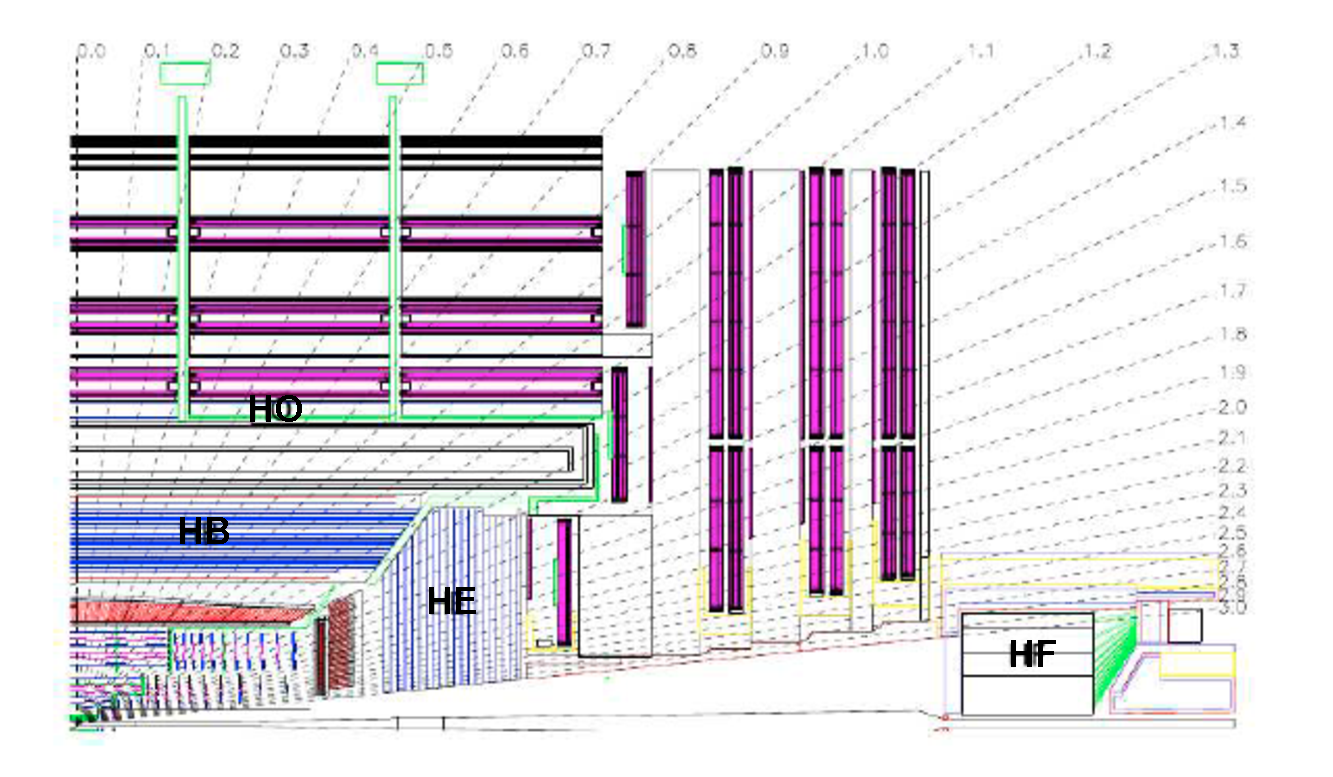
\includegraphics[width=0.8\textwidth]{Figures/Detector/HCAL}
\caption{Diagram of one quadrant in the r-$\theta$ plane showing the locations of the components of the HCAL: HB, HE, HO and HF, with lines of constant $\eta$ shown.}
\label{fig:HCAL}
\end{figure}


The barrel consists of two halves each with 18 identical azimuthal wedges, extending outwards by 0.96m. Each wedge has 17 layers of 3.7\,mm thick plastic scintillator, interspersed with brass absorber plates, with the exception of the innermost and outermost absorbers, which are made from stainless steel to add structural stability. Directly behind the ECAL is placed the first active layer, with more than double the scintillator thickness (9\,mm) to actively sample the particles traversing the support material between the ECAL and HCAL. The final layer also has this thickness to catch showers that form late in the absorber. 

A similar structure makes up each end-cap with 18 wedges dividing up the angle $\phi$ containing 19 active plastic scintillators with brass absorbers between. The number of interaction lengths travelled by particles in the HB and HE is dependent on the $\eta$ of the particle, and while it is 10 at high $\eta$, in the central region this is as low as 5. In order to compensate for this, an outer barrel detector is added in the range $|\eta| <$ 1.26 consisting of two layers of scintillating material outside the magnet, and therefore utilising the coil as an absorber. This extends the total thickness of the full calorimeter to at least 11.8 interaction lengths. 

The design of the forward calorimeters is driven by the need for radiation hardness, as the region closest to the beam line has an energy density up to seven times greater than in the central region. Thus absorbers made of stainless steel and active scintillators of quartz fibres are chosen. Twelve wedges in $\phi$ are located 11.2m from the point of interaction, with the fibres parallel to the beam.

Measurements of hadron energies in the region $| \eta| < 3.0$ rely not only on the HCAL setup described, as a significant fraction of hadrons will have begun to shower while travelling through the ECAL, which contributes around one interaction length.  The hadronic component of these showers will continue on into the HCAL, but much of the initial electromagnetic activity can be contained in the ECAL, thus use of measurements in both calorimeters are combined to reconstruct the true energy of a hadron. Using test beams over a range from 2 to 350 GeV the resolution for the reconstruction of hadron energy for the HCAL and ECAL combined is given by the following equation~\cite{HCALTestBeam}.
\begin{equation} 
\left(\frac{\sigma}{E}\right)^2 = \left(\frac{84.7\%}{\sqrt{E}}\right)^2 + \left(7.4\% \right)^2 
\label{eq:H-Res}
\end{equation}


\subsection{Muon System}

Interleaved in the iron return yoke of the detector are the components of the Muon System (MS), an important design feature giving CMS its middle initial. Many new physics signatures at high energy have final states with high momentum muons, and therefore accurately measuring these is crucial for many analyses, including Higgs and SUSY channels. As muons are high mass leptons they interact little in the calorimeters, and thus retain a high percentage of their energy by the time they reach the iron return yoke. Putting the MS here far away from the interaction point allows finer precision, utilising the high magnetic field to bend even high momentum muons, and measuring the bending angle.

Muon momentum resolution using the MS is dominated at low energies (0 $< p^{\mu}_{T} < $ 200 GeV) by the multiple scattering that occurs in the material prior to the first muon station, and therefore a better resolution could be obtained using the tracking system. However, it is possible to use the muon trajectory after the yoke to extrapolate back to the interaction point. Using the tracker and muon system together improves identification and measurements, especially as any particle detected in the MS is expected to be a muon, as other particles are stopped earlier in the detector~\cite{MuonTDR}. 

Built within the iron yoke the MS shares the same structural layout, constructed in five barrel wheels, and two end-caps, together covering the region $|\eta| < 2.4$. As a large area must be covered, a silicon based setup such as used in the inner tracker would be too expensive, hence gaseous detectors are chosen. In the barrel region ($|\eta| < 1.2$) Drift Tubes (DT) are used, and in the end-caps ($0.9 < |\eta| < 2.4$) Cathode Strip Chambers (CSC) are preferred, both of which offer good position resolution, although they have a long response time. In order to provide redundancy in the trigger system an additional third element is added in both regions, the Resistive Plate Chambers (RPC). These have a worse position resolution but benefit from a much shorter response time suited to identifying the bunch crossing. Combining the information from these complimentary RPCs with the DTs and CSCs gives rise to an efficient and robust trigger. The arrangement of the muon system is shown in Figure~\ref{fig:MuonSystem}, with the locations of each type of detector shown.

\begin{figure}
\centering
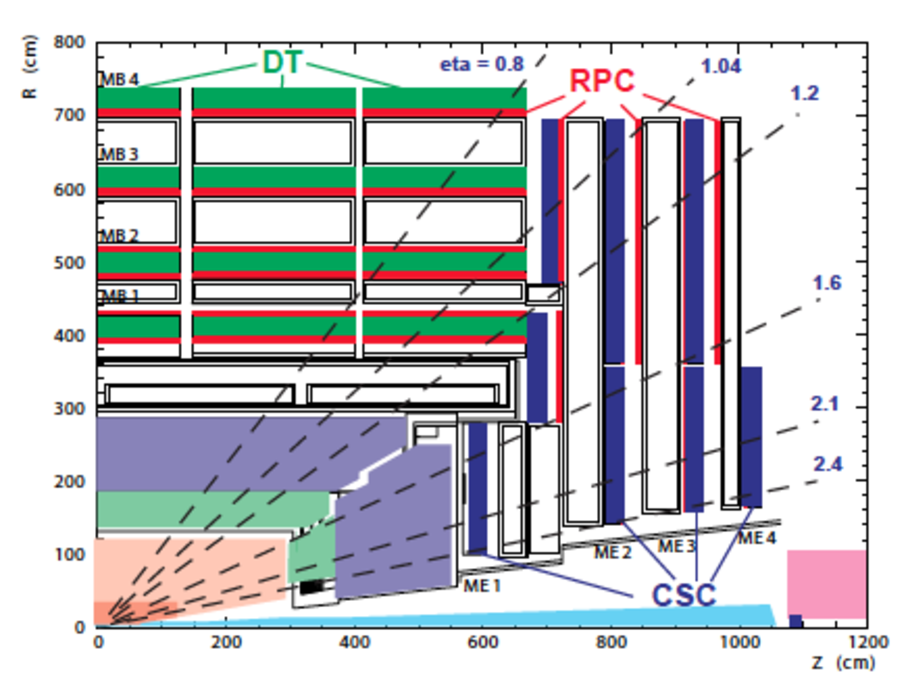
\includegraphics[width=0.6\textwidth]{Figures/Detector/MS}
\caption{The Muon system shown in the $r-\theta$ plane showing the three components and their locations. Lines of constant $\eta$ are indicated for reference.}
\label{fig:MuonSystem}
\end{figure}

In the barrel, the magnetic field is uniform, and therefore allows the use of Drift Tube chambers.  Each of the five wheels are made up of 12 sectors, containing four chambers apiece, making up a full barrel of 240 chambers. The inner three chambers consist of three Super Layers (SL) using the first and third for the $\phi$ coordinate measurement and the second for the $z$ coordinate. In the outer chamber,  there are only two SLs and these contribute only to the $\phi$ measurement. Four layers of drift tubes make up a SL, and each layer is shifted by half a cell from the one beneath, to ensure any particle trajectory meets some active material. Each tube contains an anode wire and cathode strips, and is filled with a gas mixture of 85\% Ar and 15\% CO$_{2}$ gas. The Ar atoms are ionised by a charged particle, and the resulting electrons and ions drift towards the anode and cathodes. Electrons reaching the wire are extremely excited by the high density field, which allows them to ionise further molecules, known as the ``avalanche effect". Thus an electrical signal large enough to be measured is produced. The drift distance is 21\,mm and the drift time is limited to $\sim$\,380\,ns by the gas chosen, corresponding to 16 bunch crossings.

Due to the aforementioned solenoidal magnetic field, the end-caps experience an irregular magnetic field, and a higher expected particle flux, and therefore drift tubes are not suitable. In this region 468 Cathode Strip Chambers are used, set out perpendicularly in four stations in each end-cap. Trapezoidal chambers consist of seven radially oriented cathode strips, and in between six planes of azimuthal anode wires. The gas filling the gaps is made up of 40\% Ar, 50\% CO$_{2}$ and 10\% CF$_{4}$, and the chambers work much in the same way as the DT's, with a high voltage applied to achieve the avalanche effect. As the wires and strips are almost perpendicular its possible to make a simultaneous measurement in r and $\phi$ by identifying the charge fraction in several cathode strips. 

In addition, the complimentary system of RPCs is installed in both the barrel and end-cap regions, providing extra information in the region $|\eta| < 1.6$. In the barrel there are 480 rectangular RPCs, with two layers per station, the inner two stations have one inside and one outside the DTs, and the outer two stations having both inside. The end-caps have overlapping trapezoidal chambers in the outer two concentric rings. These parallel-plate gaseous detectors have two thin gaps between plates, which are attached to high voltage to drive avalanche mode. The avalanche reaches the plates quickly, as the gas gaps have a small width, and so the measurement is made within $\sim$\,3\,ns, much smaller than the bunch crossing. The position resolution is adequate at the same time, and so the RPCs are used to contribute to the trigger, and also to map identified muons to a particular bunch crossing.

\subsection{Trigger}
\label{sec:detrig}
When running at design luminosity, the LHC will collide protons with a bunch crossing of 25~ns, each of which will result in $\sim$\,20 interactions corresponding to a rate of 40MHz of data, or 40\,TB/s~\cite{TRIGTDR}. Not only is it impracticable for this volume of data to be stored, but much of this corresponds to unwanted events, where no new particles have been produced, as the cross-sections for interesting physics processes are several orders of magnitude lower than the inelastic p-p cross section. Hence these events must be whittled down into those which it is worthwhile to store. This is done by the trigger system that is divided into two components, the online hardware-based Level 1 Trigger (L1) which reduces the rate to that which can be routed from the buffer to the computing farm, and then the offline software-based High Level Trigger (HLT). 

The L1 trigger is driven by the amount of time that data at the incoming rate that can be stored in the buffer, before needing to be overwritten. At design luminosity this is 128 bunch crossings, $\sim$\,3\,\textmu s. Within this time the rate must be lowered to 100kHz, the acceptable rate for writing to the computing farm used for the HLT. This is accomplished using a tree system of triggers. First, the Regional Calorimeter Trigger (RCT) and Regional Muon Trigger (RMT) perform local reconstruction of objects (muons, electrons, photons, jets). The Global Calorimeter Trigger (GCT) and the Global Muon Trigger (GMT) receive these objects, and sort them using a number of criteria e.g. Energy, momentum, quality of identification. The top four of each type are sent to the Global Trigger, which uses this information along with global event measurements such as total momentum to decide if the event passes the L1 Trigger requirement. If so it is sent to the HLT, if not it is not stored and passes out of the buffer. 

The HLT essentially does the same thing as the L1 trigger, but is not driven by strict time requirements. Running on a large computer farm of multi-core computers, it has access to the entire readout data, and performs sophisticated calculations akin to those performed in physics analyses. Using partial reconstruction algorithms to clearly identify what objects are in an event, it is possible to filter according to a set of desired physics criteria.  The desired rate to store to tape is around 300Hz, and the HLT is designed and monitored constantly during data-taking to ensure the correct rate is achieved. In a given run a ``menu" of different trigger paths is included, to select different types of event and with different thresholds. Some require the presence of a certain object, such as a Muon. Others combine requirements, and these are called Cross-Triggers. For example a family of triggers exist that require a certain HT and MHT. Within this family there are several different thresholds, which go down as low as can be included in the menu without raising the rate prohibitively much. Thresholds that have a rate which is too high become ``prescaled".
\subsubsection{Prescaled Triggers}
If the rate of output of a given trigger becomes too high as the luminosity increases, the trigger will often remain in the menu with a lowered rate due to the inclusion of a ``prescale factor" $n$. The trigger is known as ``prescaled", as only 1 in $n$ events that pass the trigger requirements will be included in the trigger output, thus reducing the efficiency of said trigger by the factor $n$. 

For analysis search purposes this is undesirable as it would result in a significant loss of interesting events, but these prescaled triggers can play a part in control samples and background estimates. In these areas it is suitable to multiply the yield by the prescale factor in order to provide an estimate of actual event numbers, whereas in the signal region it is essential to treat only physical yield measurements with an un-prescaled trigger.
\subsection{Primary Dataset}
Several Primary Datasets (PD) are used to store the data, where an event is allocated to a PD based on which low-threshold trigger bits are passed in order to group like events together. For example, in this thesis the datasets used are the HT PD where events are stored that pass low requirements of missing energy, and also the Photon PD in which events have at least one photon. This is done for ease of use of the analysis user. The PDs have some overlap, therefore only one is required for a full luminosity analysis providing the offline selection is efficient to the triggers used in selection. In the analysis set out in this thesis the use of the Muon PD is rejected for the muon control sample for this reason, as the selection allows very soft muons. 



%\include{Object Reconstruction}
%\chapter{SUSY Search Topology and the $\alpha_{T}$  variable}
\cite{PRL1fb}
\cite{DawsonSearch}
\cite{1fbnote}
\cite{aTHTdepstuart}

This thesis describes an inclusive search for new physics with a signature of significant missing energy and hadronic jets. Whilst 


\section{SUSY Search Toplogies}

As previously discussed in Chapter \ref{ch:theory}, SUSY models that conserve R-Parity and therefore indicate new physics at the TeV scale introduce a candidate particle for dark matter. As this LSP cannot be observed due to its weakly interacting nature, searching for it is analogous to a search for large missing energy in particle collisions. In the CMS detector reconstruction of all visible particles allows us to calculate the transverse component of this quantity, missing $E_{T}$ or \met. 

As there are many models to describe the exact nature of SUSY due to the unknown mechanism of SUSY breaking, it is desirable to design an experimental search which does not rely on any one in particular, or even on the assumption of SUSY. These are called ``inclusive" searches, and retain sensitivity to any new physics resulting in a new particle with the properties of a WIMP. The main feature is a requirement of a large quantity of \met along with final state objects (hadronic jets, leptons, photons). The search space is then divided into channels via the final state objects required, in order to perform orthogonal searches to increase sensitivity and to allow combination 

Discussion of SUSY on the whole and specific models such as mSUGRA are then used to quantify the reach of the search and to tune the cuts with Monte Carlo data. Where no new physics is found it can be useful to set limits on the parameters of such models, and in this thesis we will use mSUGRA for this purpose, along with test points in the mSUGRA phase space. However it is important to remember that the search itself remains open and sensitive to any WIMP candidate. 

Physics at the LHC will suffer from high background rates, especially those from QCD, and the main goal of any analysis is selecting the new physics events required whilst removing the background from Standard Model processes. Missing energy can be observed in events in two ways, real missing energy from the production of weakly interacting particles, such as neutrinos and LSP's, and fake missing energy which is a result of mismeasurment of objects, or missed objects. 

Having noted that the generic signal produced by any such new physics model is a large amount of \met, it might be assumed this forms the main variable to separate signal from background events. As \met is measured in the calorimeters, it can be affected by miscalibration and noise in the detector, thus is not robust for early physics at the LHC. 

To combat this issue there is also the quantity \mht which represents the vector sum of transverse momenta $p_{T}$ of the jets in the system, giving the hadronic missing energy analogous to \met in a hadronic search. However, there are limitations to the use of either of these quantities, as they are not robust to mismeasurments of the jets. 

\section{$\alpha_{T}$ in a di-jet system}

The first step in devising a SUSY search strategy begins with the simplest of channels, the ``diet" search with just two jets and missing energy corresponding to two missing neutralinos. Due to the low multiplicity it is easy to understand kinematically the situation in play. Instead of using \met as the discriminating variable, it is possible to obtain a higher signal to background ratio $\sfrac{S}{B}$ using a new variable proposed by Randall and Tucker-Smith, $\alpha$, defined in Equation \ref{eqn:alpha}~\cite{Randall}. 


\begin{equation}
\alpha = \frac{E_{T}^{j2}}{M_{inv}^{j1,j2}}
\label{eqn:alpha}
\end{equation}

The $E_{T}^{j2}$ is the transverse energy of the second jet (the lowest in energy) and $M_{inv}^{j1,j2}$ is the invariant mass of the dijet system. The design of this variable allows us to exploit the expected back-to-back nature of any diet from QCD. Thus a well-measured QCD event can only take values of $\alpha < 0.5$. In sharp contrast, a SUSY event can, due to the unseen neutralinos, produce jets in a similar direction with a low invariant mass giving rise to high values of $\alpha$.

The transverse variant of this variable, given in Equation \ref{eqn:alpha} makes use of the transverse mass $M_{T}$ of the two jets as opposed to the invariant mass.

\begin{equation}
\alpha-{T} = \frac{E_{T}^{j2}}{M_{T}} 
\label{eqn:alphat}
\end{equation}

In this case a well-measured QCD event will have exactly 0.5. While both show equally strong power of background discrimination, $\alpha_{T}$ has greater signal retention for certain mSUGRA points,\cite{PASaT} and therefore is deemed comparable or superior. It is upon this variable that the search strategy is formed. The presence of the second jet energy in the numerator also gives rise to one of the most important properties of this variable, its resilience to jet mismeasurment. If there is a large mismeasurment of one of the jets, the order could be inverted. As a perfectly measured QCD event yields \alt = 0.5, the cut chosen is \alt > 0.55 in order to take into account the finite resolution of the jet energy measurement.  

 It is worth noting also that in the massless limit this may be re-written in terms of the azimuthal angle between the two jets, $\Delta \phi$ as in Equation \ref{eqn:alphatphi}. This relationship indicates a high correlation, and thus a cut on \alt renders a further cut on $\Delta \phi$ negligible\cite{ANaT}.

\begin{equation}
\alpha_{T} = \frac{\sqrt{E_{T}^{j2}/E_{T}^{j1}}}{2(1- \textrm{cos} \Delta \phi)} 
\label{eqn:alphat}
\end{equation}


\section{$\alpha_{T}$ in a n-jet system}
More complicated decay processes result in hadronic signatures with more than two jets, generalised to the n-jet system, for example where a gluino-squark pair decay to produce three quarks and two LSP's. Following the success of the construction of the \a\t variable in the diet topology, the variable was extended to apply firstly to 3-jet systems and then in a general form applicable to an n-jet system, thus incorporating the full hadronic SUSY search channel\cite{ANnaT} . This is undertaken by modelling the system of $n$ jets as though it were a diet system, through the mathematical construction of two pseudo jets. Thus \alt can be calculated using the properties of the pseudo jets. 




\section{$\alpha_{T}$ search strategy}


%\chapter{Searching for Supersymmetry with $\alpha_{T}$ in all-hadronic events}
The analysis presented here represents a model-independent search for new physics in the all-hadronic channel, where the final state is defined by the presence of jets and missing energy. Designed to search for signs of supersymmetry whilst remaining sensitive to other new physics models, an inclusive strategy is used imposing restrictions only on the final state.  Events are chosen based on their compatibility with a topology of heavy new particles pair-produced in p-p collisions, which decay through a chain with an end product which is stable and undetectable. 

Isolating these new physics events from Standard Model background processes is essential in order to identify an excess. Controlling the dominant background from QCD Multijet processed is the central feature of the strategy, implementing use of the powerful discriminant, the \alt variable described in Chapter \ref{ch:at}. The remaining backgrounds from electroweak processes may then be accounted for using data-driven estimation techniques in muon and photon control samples. 



\section{Samples}
This analysis uses datasets both from Monte Carlo simulation (MC) and of data recorded by the CMS detector in 2011.

\subsection{Monte Carlo Simulation}
Datasets of simulated events with calculated cross-sections are required for any analysis at the LHC. Due to the hadron-collider nature these rely on the PDF's 
\subsubsection{Standard Model Background}
\subsubsection{CMSSM SUSY Signal}
For the purpose of understanding the possible yields from CMSSM SUSY, two mSUGRA parameter points are used. CMS has a dedicated set of 10 Low Mass(LM) points designed for initial data-taking from which we have chosen LM4 and LM6, the values of which are found in Table~\ref{tab:LM}. 

\begin{table}[htbp]
\centering
\begin{tabular}{c c c c c c }
\hline
\hline
\textbf{mSUGRA Point} & $m_{0}$ & $m_{1/2}$ & $A_{0}$ & tan $\beta$ & sign$(\mu) $  \\
\hline
\hline
\textbf{LM4} & 210 GeV & 285 GeV  & 0 & 10 & + \\
\textbf{LM6} & 85 GeV & 400 GeV & 0 & 10 & +\\
\hline
\end{tabular}
\caption{\label{tab:LM}The two CMSSM SUSY signal points used and their corresponding mSUGRA parameter values.}
\end{table}

These points are chosen for their existence above the exclusion limit set previously, shown in Figure~\ref{fig:lm35limit} on the exclusion plot from the 2010 iteration of this analysis\cite{35paper}.

\begin{figure}[htbp]
\centering
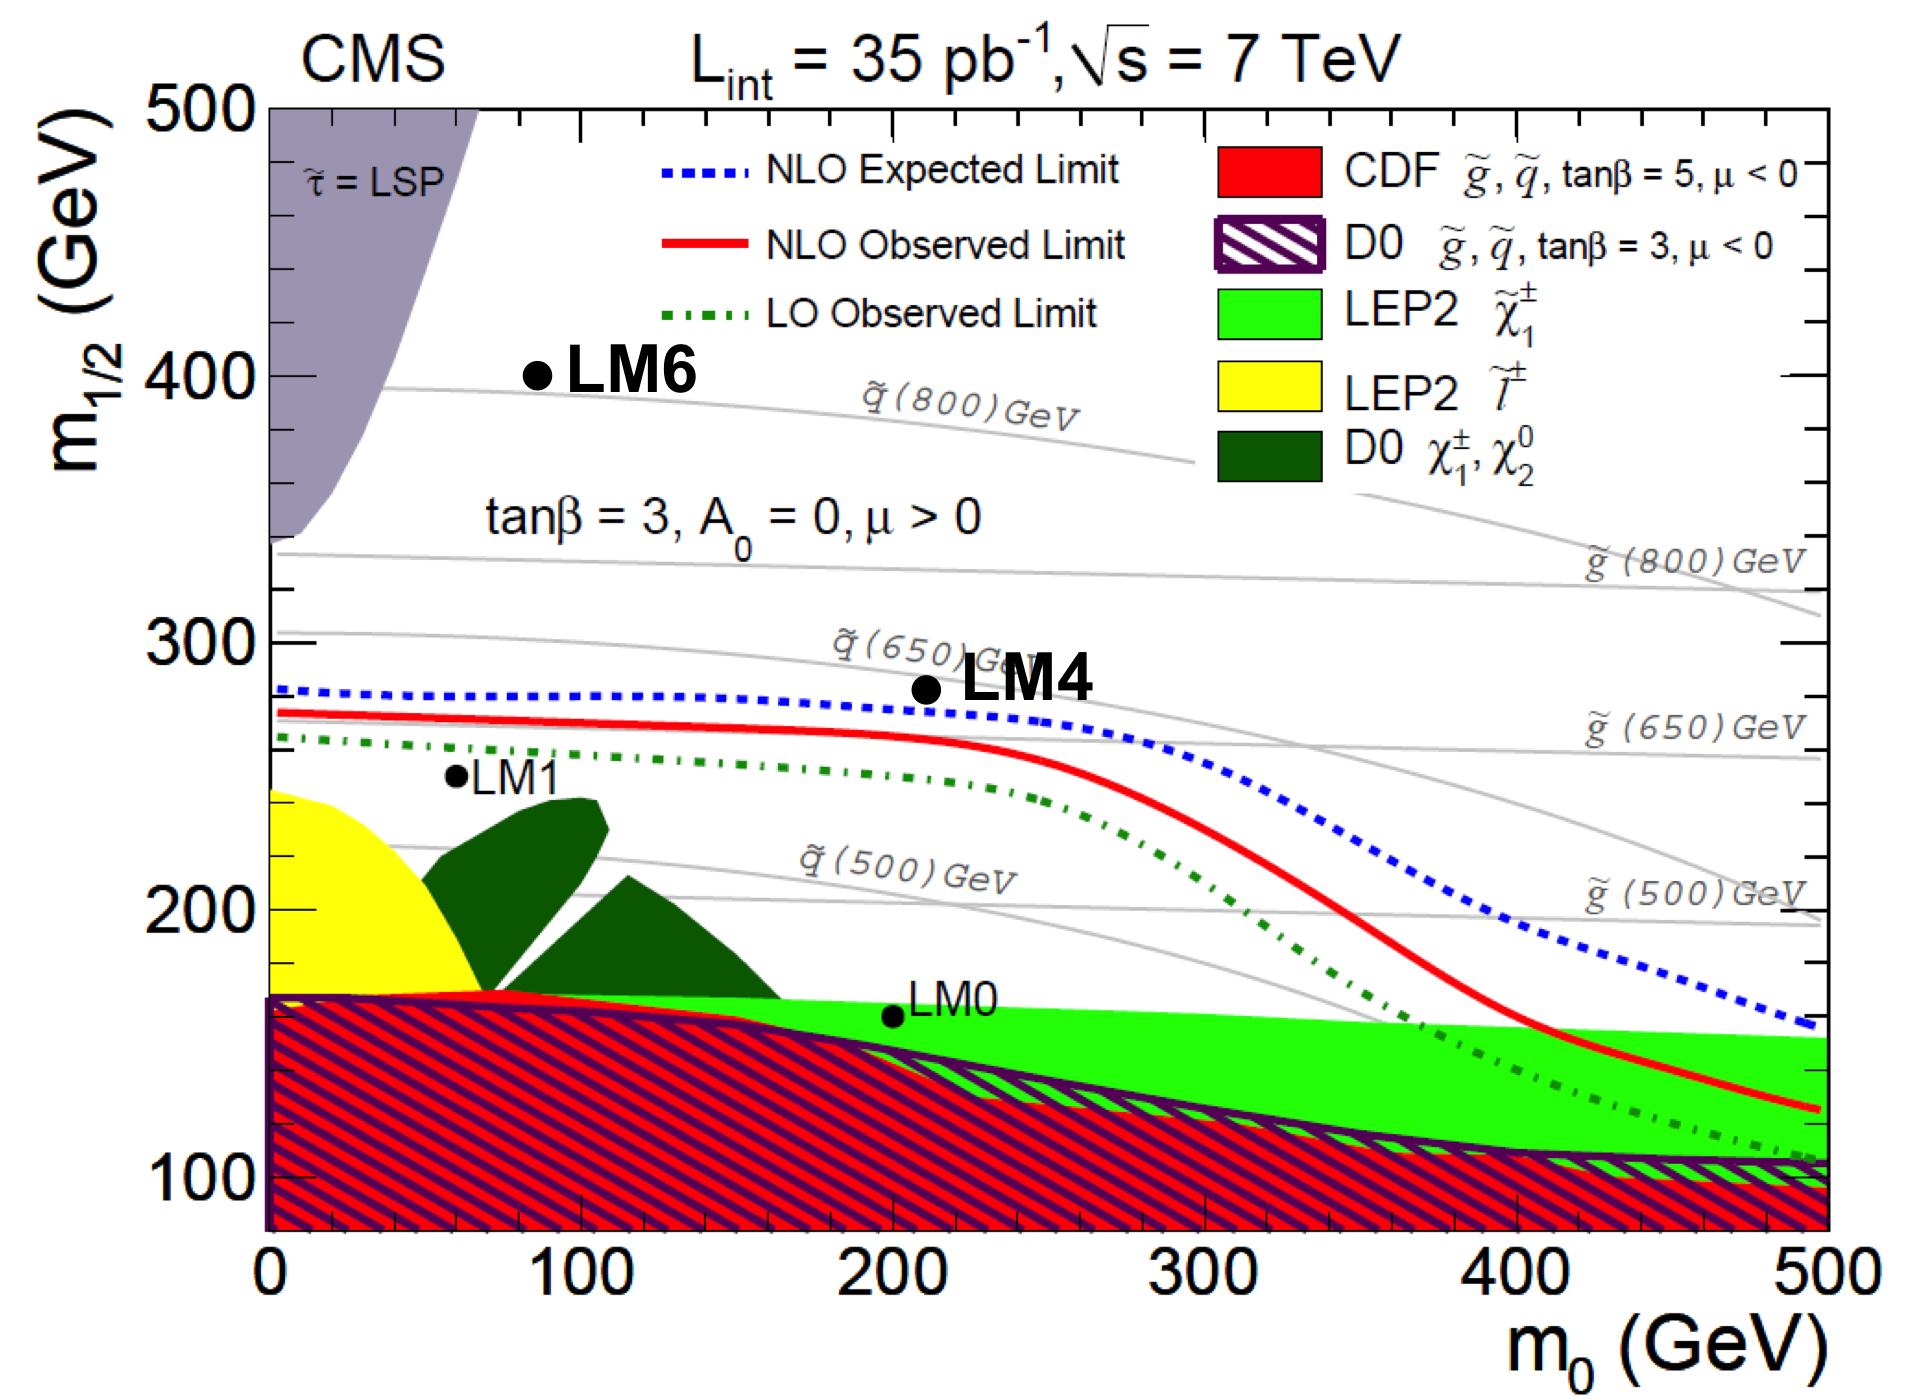
\includegraphics[width=0.70\textwidth]{Figures/Analysis/LM46on35limit}
\caption{\label{fig:lm35limit}The exclusion limit set in the previous incarnation of this analysis with the 35pb$^{-1}$ 2010 CMS dataset shown in the $m_{0}-m_{1/2}$ plane with tan $\beta$ = 10, $A_{0}$ = 0 and sign$(\mu)$ = +. Reference points LM4 and LM6 to be used in the 2011 analysis are illustrated, in the region yet to be excluded. Previously used reference points LM0 and LM1 are shown below the limit already excluded~\cite{35paper}.}
\end{figure}

The 
\subsection{Data Sample}
This analysis considers data collected by CMS at $\sqrt{s} = 7$~TeV in 2011 between March and June, during the data-taking period known locally as Run2011A. Analyses use only the data taken whilst CMS was fully operational, and thus the data used were specified by the certified list of ``good runs" that correspond to 1.1$fb^{-1}$ of integrated luminosity. 

As described previously, loose requirements on the types of triggers passed allow the sorting of the data into each Primary Dataset (PD). For the hadronic analysis the HT dataset is used, with basic low-threshold $\HT$ triggers required. Higher threshold triggers are applied subsequently as part of the analysis selection, detailed in Section~\ref{sec:trig}. 

For the data-driven estimation techniques muon and photon control samples are defined. For the muon control sample, the HT PD is also used, as a low muon $p_{T}$ requirement makes this better suited than the dedicated Muon PD. However the photon control sample uses the dedicated Photon PD that requires some basic threshold photon triggers to be passed. 



\section{Trigger}
\label{sec:trig}
In order to select the signal events and minimise the contamination from backgrounds, a set of selection criteria is applied. As described previously in Section , data collected by the CMS detector is stored and organised according to the L1 and HLT trigger paths passed. Each given dataset then undergoes the offline event reconstruction described in Chapter RECON/IDEN, after which n-tuples are constructed from which we apply cuts on objects and analysis variables. 

Previous incarnations of this analysis for the 2010 dataset REFF used a set of pure \HT triggers, however these are unsuitable for the 2011 analysis as these have too high thresholds for the analysis due to the increase in instantaneous luminosity. The use of cross-object triggers is now  employed, requiring events that pass thresholds in both \HT and \mht for the signal region, and using the lowest un-prescaled thresholds available to ensure signal yields are accurate. 

As this analysis makes use of those events which fail the selection criteria also, the hadronic control sample, the pre-scaled \HT triggers are still used taking into account the pre-scaled factors. In the muon control sample, due to the low \Pt threshold we use the same triggers as for the hadronic signal sample, and the photon sample makes use of the single photon trigger paths. 




Having passed one of the un-prescaled triggers the events are subjected to a series of cuts on objects and analysis variables in order to select the event topologies required and minimise the background contamination. 
\section{Object Definitions}

\subsection{Jets}
\label{sec:jetsel}
The jets used in this analysis are Calo Jets, reconstructed as described in Section~\ref{sec:reconjet} using the anti-k$_{T}$ jet clustering algorithm. In addition, a reconstructed jet must pass an additional selection in order to be considered for the analysis:
\begin{itemize}
\item Corrected jet transverse momentum requirement of \Pt $>$ 50~GeV 
\item Jet pseudo-rapidity $|\eta| < 3$ required to ensure within the fiducial range of the calorimeter systems. 
\item Passes``loose" jet identification criteria to reject jets resulting from unphysical energy using cuts in Table \ref{tab:jetid}. 
\end{itemize}

\begin{table}[htbp]
\centering
\begin{tabular}{ m{6.6cm}  c  c }
\hline
\hline
 \centering Definition & Variable & Cut \\
\hline
\hline
 \centering Fraction of jet energy contributed by the ``hottest" hybrid photo-diode &  $f_{HPD}$ & $< 0.98$ \\
 %\hline
 \centering Minimum number of cells required to contribute 90\% of the jet energy & $N^{90}_{cells}$ & $\leq$ 2 \\
 %\hline
 \centering Fraction of jet energy contributed by deposits in ECAL & $f_{EM}$ & $> 0.01$ \\
 %\hline
\multirow{2}{6.9cm}{Balance of the energy measured in the short($E_{S}$) and long$(E_{L})$ HF fibers.} &  $R_{HF} = \frac{(E_{S} - E_{L})}{ (E_{S} + E_{L})}$ & $R_{HF} > - 0.9$\\
& (if  $p_{T}^{jet}>$ 80~GeV)  &             ($-0.9 < R_{HF} < 1$)\\
\hline
\end{tabular}
\caption{\label{tab:jetid} Set of cuts applied in ``loose" CaloJet ID used to reject jets resulting from fake calorimeter deposits representing unphysical energy. Devised using cosmic run data as a pure sample of non-collider ``fake" jets, full details of which can be found in \cite{JME-09-008}}
\end{table}


Any jet which pass the $\Et$ and $\eta$ requirements but fails the ``loose" identification criteria is noted, and the event is marked as containing an ``odd" jet, as the presence of such a particle reflects an event whose kinematics are poorly understood and may therefore lead to a misleading \MHT.
\subsection{$\HT$ and \MHT}
The calculation of both \HT and \MHT is performed using only the jets selected by the selection above in Section~\ref{sec:jetsel}.

\subsection{Muons} 
Although muons are not required by the analysis, a veto on them must be employed, based on muons that satisfy the following set of criteria:
\begin{itemize}
\item $p^{\mu}_{T} >$ 10~GeV
\item $| \eta|$ $<$ 2.5
\item Relative Combined Isolation = $(Iso_{tracker} + Iso_{ECAL} + Iso_{HCAL}) / p^{\mu}_{T} < $0.15\footnotemark
\item Passes ``tight" muon identification, using cuts shown in Table~\ref{tab:muid}.
\end{itemize}
\footnotetext{The components $Iso_{tracker}$($Iso_{ECAL}, Iso_{HCAL})$ represent the sum of \Pt($E_{T}$) in the relevant detector component, calculated in a cone of R = 0.3 in $\eta-\phi$ around there muon trajectory. The track hits used to reconstruct the muon are not used and any muon deposit in the calorimeters is removed via a smaller veto cone.}

\begin{table}[htbp]
\centering
\begin{tabular}{ m{8.9cm}  c  c }
\hline
\hline
 \centering Definition & Variable & Cut \\
\hline
\hline
 Reconstructed with outside-in algorithm & Global Muon & Required\\
  %\hline
Reconstructed with inside-out algortithm & Tracker Muon & Required\\
% \hline
 Global muon track fit quality & $\chi^{2}$ & $< 10$ \\ 
 %\hline
Number of hits in the silicon tracker included in track & $N^{hits}_{\textit{trk}}$ &$ >$ 10\\
%\hline
Number of pixel hits in $N^{hits}_{trk}$ & $N^{hits}_{\textit{pixel}}$ & $ > $ 0\\
Number of hits in muon system included in Global Muon & $N^{hits}_{\textit{muon}}$ & $\geq $ 1\\
Transverse impact parameter with respect to vertex & $d_{xy}$ & $< $ 2~mm\\
\hline
\end{tabular}
\caption{\label{tab:muid} Set of cuts applied in ``tight" Muon ID, taken from \cite{MUO-10-002}}
\end{table}



\subsection{Electrons}
Similarly electrons are also defined for veto purposes, with the definition of an electron in the analysis as that passing the following cuts:

\begin{itemize}
\item $E^{e}_{T} > 10 GeV$
\item $|\eta| < 2.5$
\item Combined Isolation = $(\sum_{tracker} p_{T} + \sum_{ECAL}E_{T} + \sum_{HCAL}E_{T})/p^{e}_{T} < 0.15$
\item Pass WP95 electron identification implemented using cuts in Table~\ref{tab:eid}.
\end{itemize}

\begin{table}[htbp]
\centering
\begin{tabular}{ m{6.9cm}  c  c  c}
\hline
\hline
 \centering Definition & Variable & Barrel Cut & End-Cap Cut \\
\hline
\hline
RMS of the width in $\eta$ of the crystals about the most energetic crystal in the seed& $\sigma_{i \eta i \eta}$ & $<$ 0.01 & $<$ 0.03\\
Difference in $\phi$ between track and supercluster&$\Delta \phi_{vtx}$& $<$ 0.8 & $<$ 0.7 \\
Difference in $\eta$ between track and supercluster& $\Delta \eta_{vtx}$& $<$ 0.007 & $<$ 0.01\\
Ratio of HCAL energy in $\Delta R = 0.15$ to ECAL seed energy & H / E & $<$ 0.15 & $<$ 0.07\\
\hline
\end{tabular}
\caption{\label{tab:eid} Set of cuts applied in ``WP95" Electron ID, taken from \cite{AN-10-116} corresponding to an intended 95\% efficiency for signal electrons in W events for electrons with $p_{T} > 20$~GeV.}
\end{table}
\footnotetext{where electron $p_{T} > 20$~GeV, measured with a sample of $W \ra e$ events.}
\subsection{Photons}

Photons in the analysis are defined by the following set of requirements:
\begin{itemize}
\item $p_{T}^{\gamma} > $ 25~GeV
\item $|\eta| < 2.5$
\item Passes ``tight" photon cut-based identification (including isolation) using cuts shown in Table~\ref{tab:pid}.
\end{itemize}


\begin{table}[htbp]
\centering
\begin{tabular}{ m{6.9cm}  c  c  c}
\hline
\hline
 \centering Definition & Variable & Barrel Cut & End-Cap Cut \\
\hline
\hline
Tracker Isolation in a cone of R=0.4 & $Iso_{trk}$ & \multicolumn{2}{c}{$< (2.0 GeV + 0.001E_{T}^{\gamma})$}\\
ECAL Isolation in an outer cone of R=0.4 (inner cone R=0.06 removed). & $Iso_{ECAL}$ & \multicolumn{2}{c}{$< (4.2 GeV + 0.006E_{T}^{\gamma})$}\\

HCAL Isolation in an outer cone of R=0.4 (inner cone R=0.15 removed). & $Iso_{HCAL}$ & \multicolumn{2}{c}{$< (2.2 GeV + 0.0025E_{T}^{\gamma})$}\\

RMS of the width in $\eta$ of the crystals about the most energetic crystal in the seed& $\sigma_{i \eta i \eta}$ & $<$ 0.013 & $<$ 0.030\\
Ratio of HCAL energy in $\Delta R = 0.15$ to ECAL seed energy & H / E & $<$ 0.05 & $<$ 0.05\\
\hline
\end{tabular}
\caption{\label{tab:pid} Set of cuts applied in ``tight" Photon ID, taken from \cite{EGM-10-006}}
\end{table}

\section{Pre-Selection}
A basic selection of events used for comparison of distributions between data and monte-carlo events shall be known as "pre-selection",  following the details set out in this section.

\begin{description}
\item[Vertex Requirement]{It is required that events have at least one non-fake good primary vertex with $N_{dof}$ $>$ 4. Constraints on the vertex position along the beam axis $|z_{vtx}| <$ 24 cm and perpendicular to the axis of $\rho <$ 2 cm must be satisfied. Events that have many fake tracks are identified as monster events and removed, by requiring that the ratio of High Purity tracks to the total number be greater than 25\% in events with more than 9 tracks. }

\item[HCAL Barrel and End-cap (HBHE) Noise Fiter]{Events where noise has been identified in the HCAL are removed also, using an algorithm which checks for Photodetectors which have at east 17 out of 18 channels with an E $>$ 1.5 GeV.}
\end{description}
Following these conditions events are then selected by the following criteria, using the definitions of physics objects according to the criteria stated previously:

\begin{itemize}
\item Pass triggers as detailed in Section~\ref{sec:trig}
\item{Require events with N$_{jet}$ $\geq$ 2}
\item N$_{muon}$ = N$_{electron}$ = 0 to reduce the effects of missing energy from neutrinos.
\item N$_{photon}$ = 0 to ensure a pure hadronic set of events.
\item Events with $>$ 0 ``odd" jets are vetoed.
\item Additional constraint on the transverse momentum of the two leading jets $p^{j1}_{T},p^{j2}_{T} >$ 100~GeV.
\item Additional constraint on the leading jet pseudorapidity $|\eta^{j1}| <$ 2.5.
\item \HT $\geq$ 275 GeV 
\item{To protect the quantity \alt from the scenario where many jets exist below the momentum acceptance threshold, the missing energy variable \mht estimated from jet measurment is compared to the quantity \met measured from the calorimters. If the ratio R$_{miss}$ = \mht / \met $>$ 1.25, the event is rejected. 
}
\item \alt $>$ 0.55
\end{itemize}




\section{An $\HT$ Shape Analysis}

Previous iterations of this analysis strategy with the 35pb$^{-1}$ 2010 LHC dataset \cite{35paper} used a cut-and-count strategy for all events passing the selection, defining the signal region by an $\HT > 375$ and using lower regions in \HT as control regions. The 2011 analysis follows the same selection but motivated by the increasing luminosity is undertaken as a Shape Analysis in bins of \HT, using the whole range $\HT > $275 GeV as a signal region. This allows greater sensitivity to states of higher mass. 

The set of lower bin edges are as follows: [275,325,375,475,574,675,775,875], where each bin is exclusive with an upper limit corresponding to the lower edge of the next bin, except in the case of the final bin which is inclusive $\HT > $875. The background estimation techniques employed from data therefore are designed to identify the contribution in each distinct bin. 

In order to include the two lowest bins in \HT is is necessary to scale the jet thresholds stated in Section \ref{sec:press} in order to maintain even event kinematics allowing a shape analysis approach. The background from $t\bar{t}$ + jets carries a bias to higher jet multiplicities compared to the other EWK components, and thus with identical jet definitions exhibits a turn on behaviour in \HT. In order to remedy this, the lowest two bins have the two jet energy requirements scaled by $\sfrac{l}{375.}$ where $l$ represents the bin lower edge in question. This leads to the thresholds in Table~\ref{tab:thresh}.

\begin{table}[htpb]
\centering
\begin{tabular}{c c c}
\hline
\hline
\HT Region & Jet Definition & Second-Leading Jet Cut \\
\hline
\hline
275 $<$ \HT $<$ 325 & $p_{T} >$ 36.7~GeV & $p^{j1}_{T}, p^{j2}_{T} >$  73.3~GeV\\
325 $<$ \HT $<$ 375 & $p_{T} >$ 43.3~GeV & $p^{j1}_{T}, p^{j2}_{T} >$ 86.7~GeV\\
\HT $>$ 375 & $p_{T} >$ 50~GeV & $p^{j1}_{T}, p^{j2}_{T} >$  100~GeV\\
\hline
\end{tabular}
\caption{\label{tab:thresh}The three different regions of jet scaling, with values indicated both for the basic definition of a jet used in the analysis, and the second-to-leading jet energy cut. The former is especially important as this alters the value of \HT as this is calculated using the jets in the event.}
\end{table}

\section{Data to Monte-Carlo Comparisons }




\begin{figure}[h]
\centering
\subfigure[Comparison of $H_{T}$ between data and MC for the hadronic selection for $H_{T}$ $\geq$ 375 GeV and MHT $>$ 100 GeV.]{\label{fig:figures_HT_all}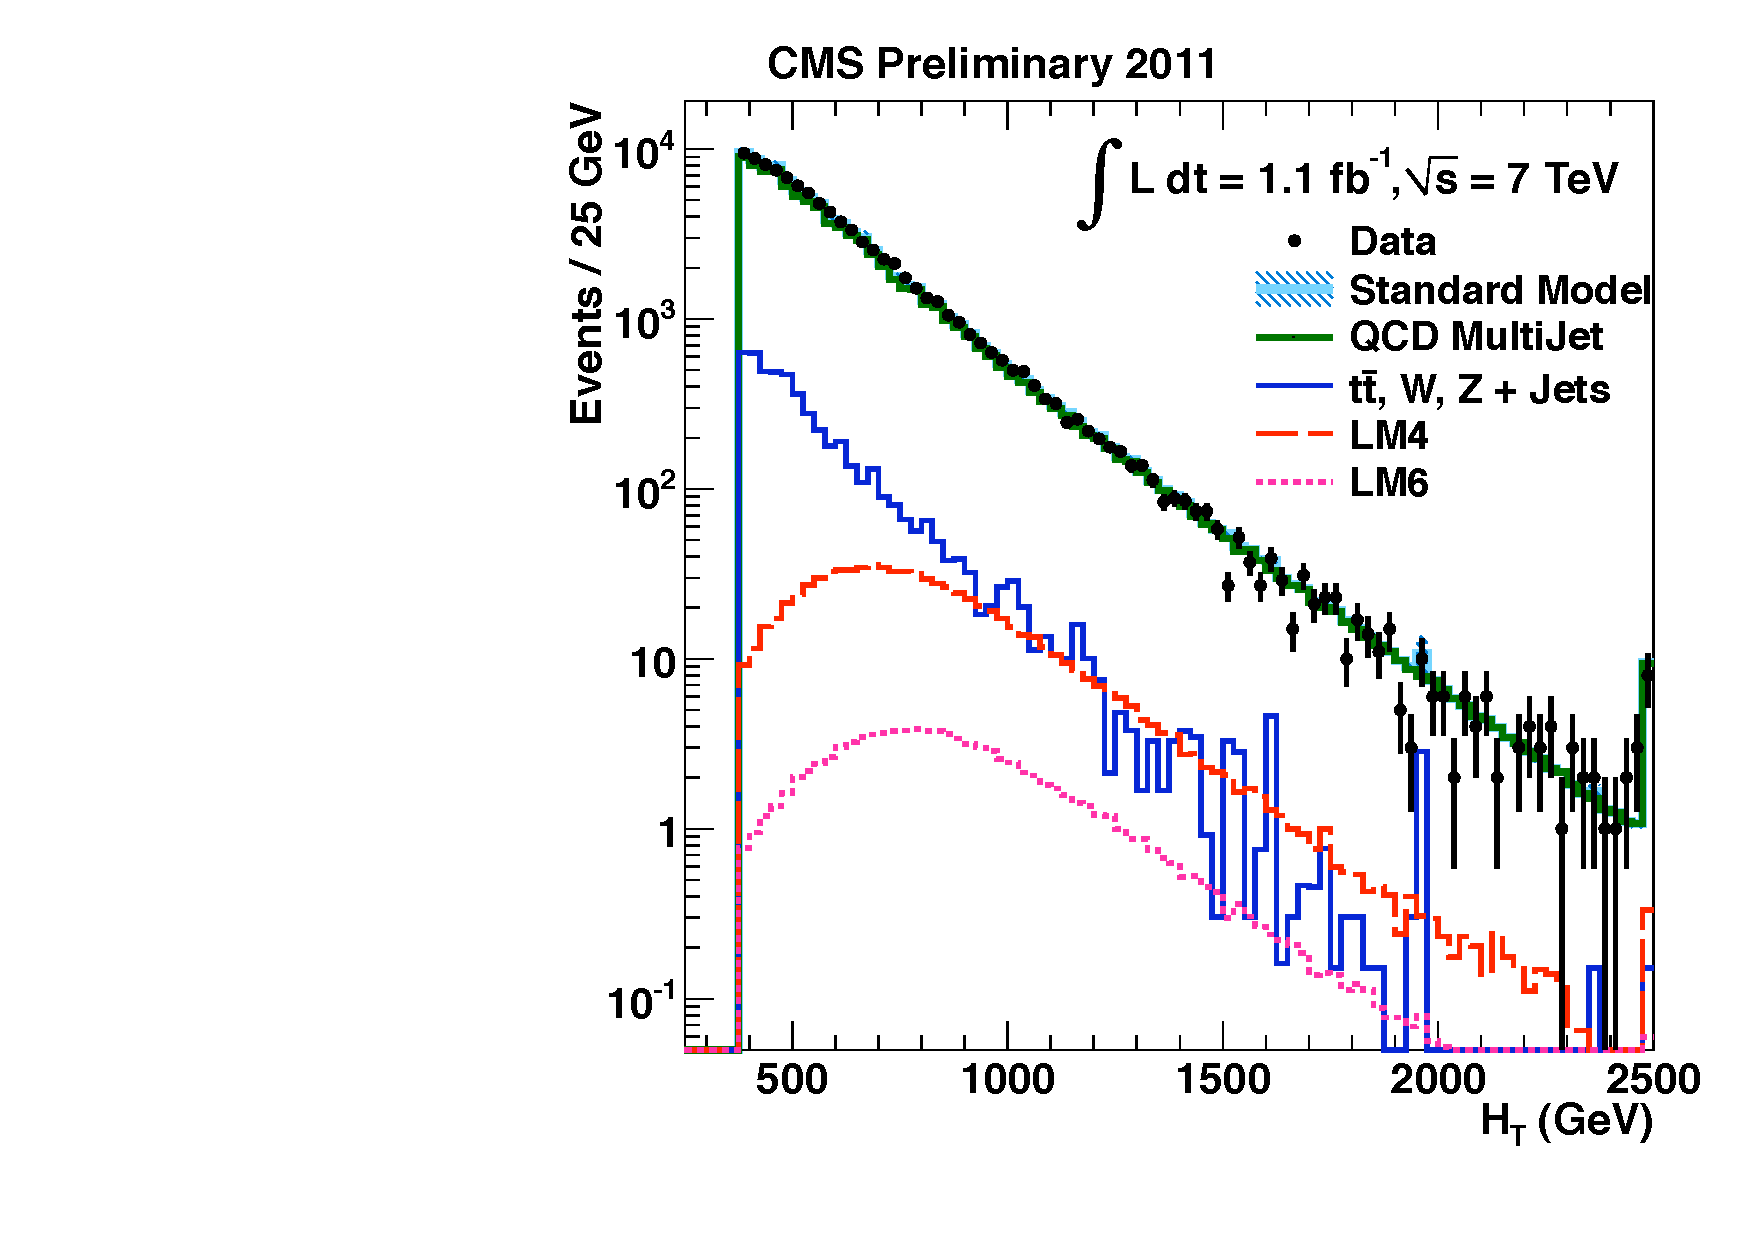
\includegraphics[width=0.40\textwidth]{Figures/Analysis/PAS/HT_all.pdf}}
\subfigure[Comparison of the jet multiplicity between data and MC for the hadronic selection, for $H_{T}$ $\geq$ 375 GeV and MHT $>$ 100 GeV.]{\label{fig:figures_JetMultiplicity_all}
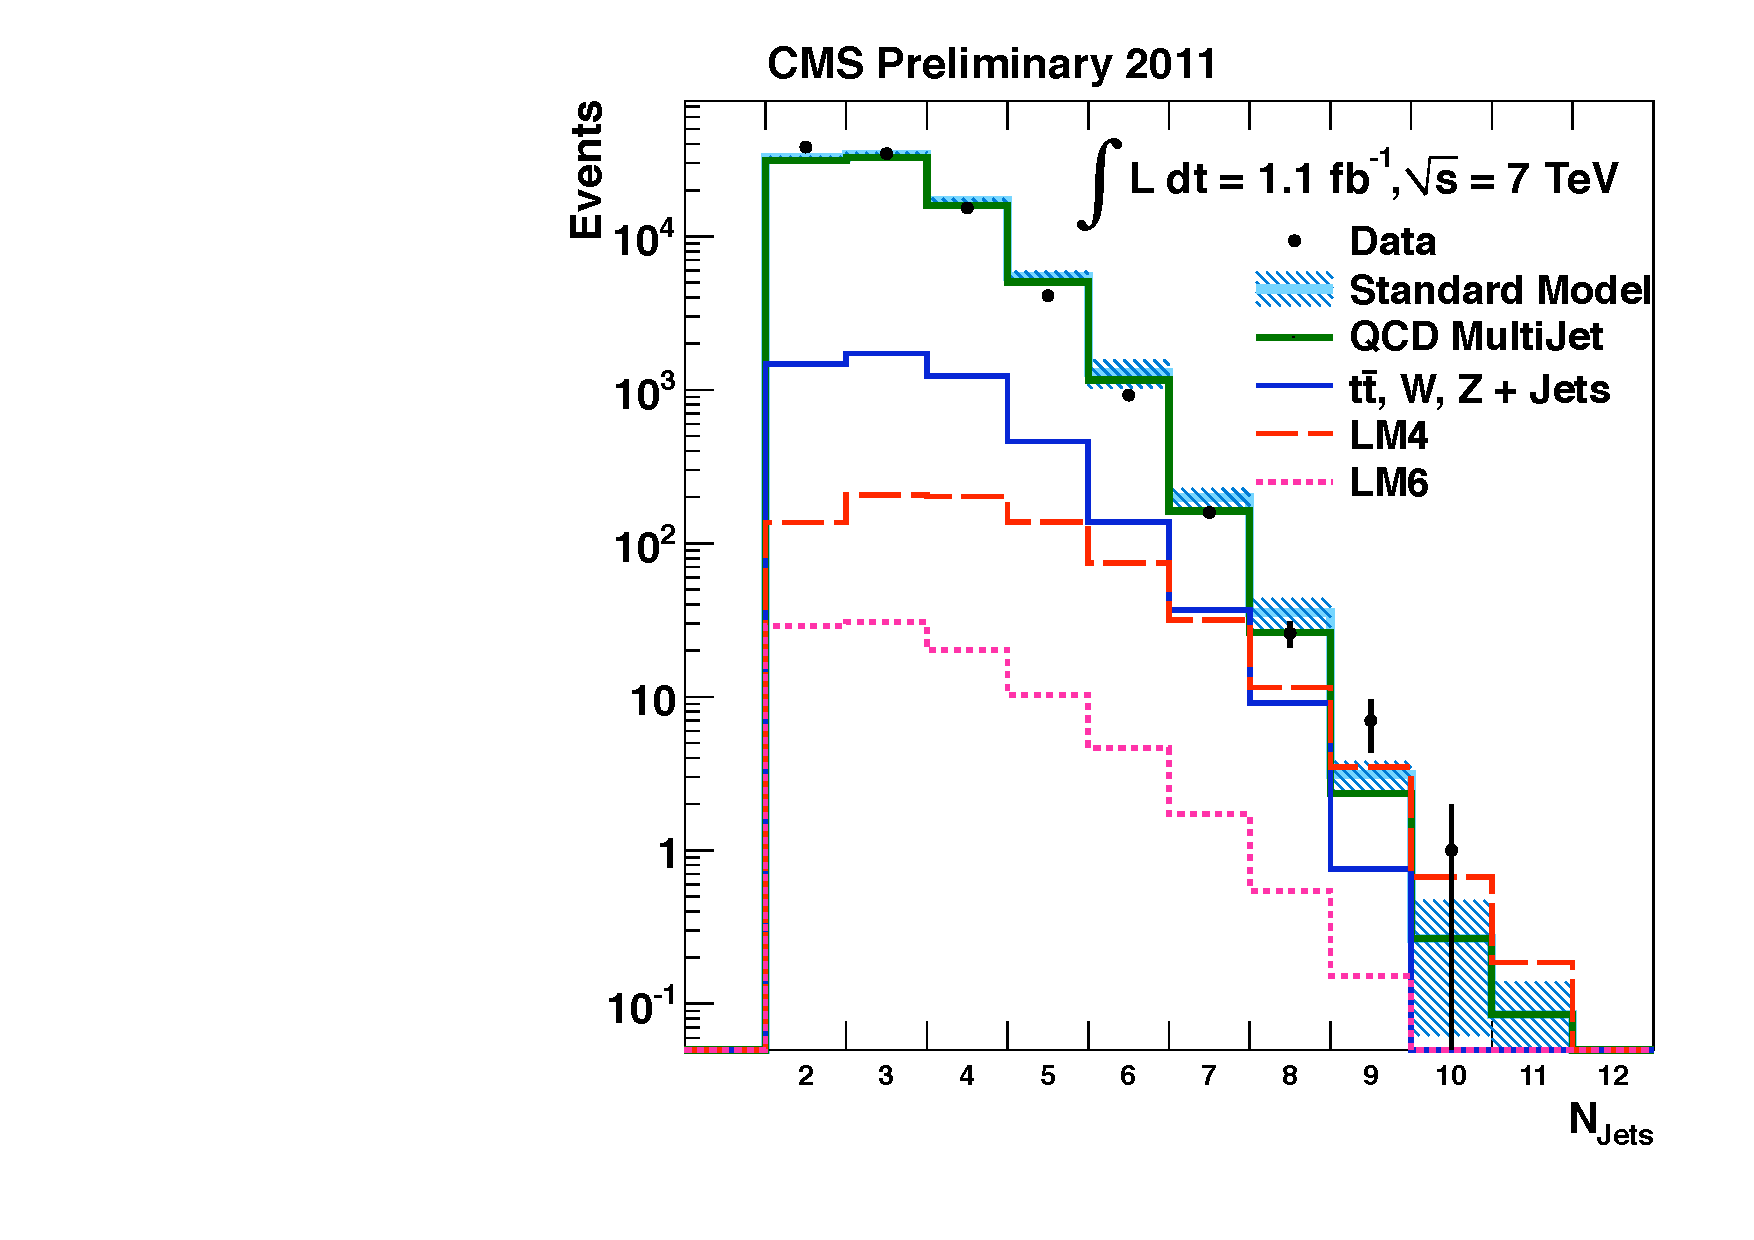
\includegraphics[width=0.40\textwidth]{Figures/Analysis/PAS/JetMultiplicity_all.pdf}
}
 \newline
\subfigure[Comparison of the $\alpha_{T}$ distribution between data and MC for the hadronic selection, for $H_{T}$ $\geq$ 375 GeV and MHT $>$ 100 GeV.
]{\label{fig:figures_AlphaT_all}
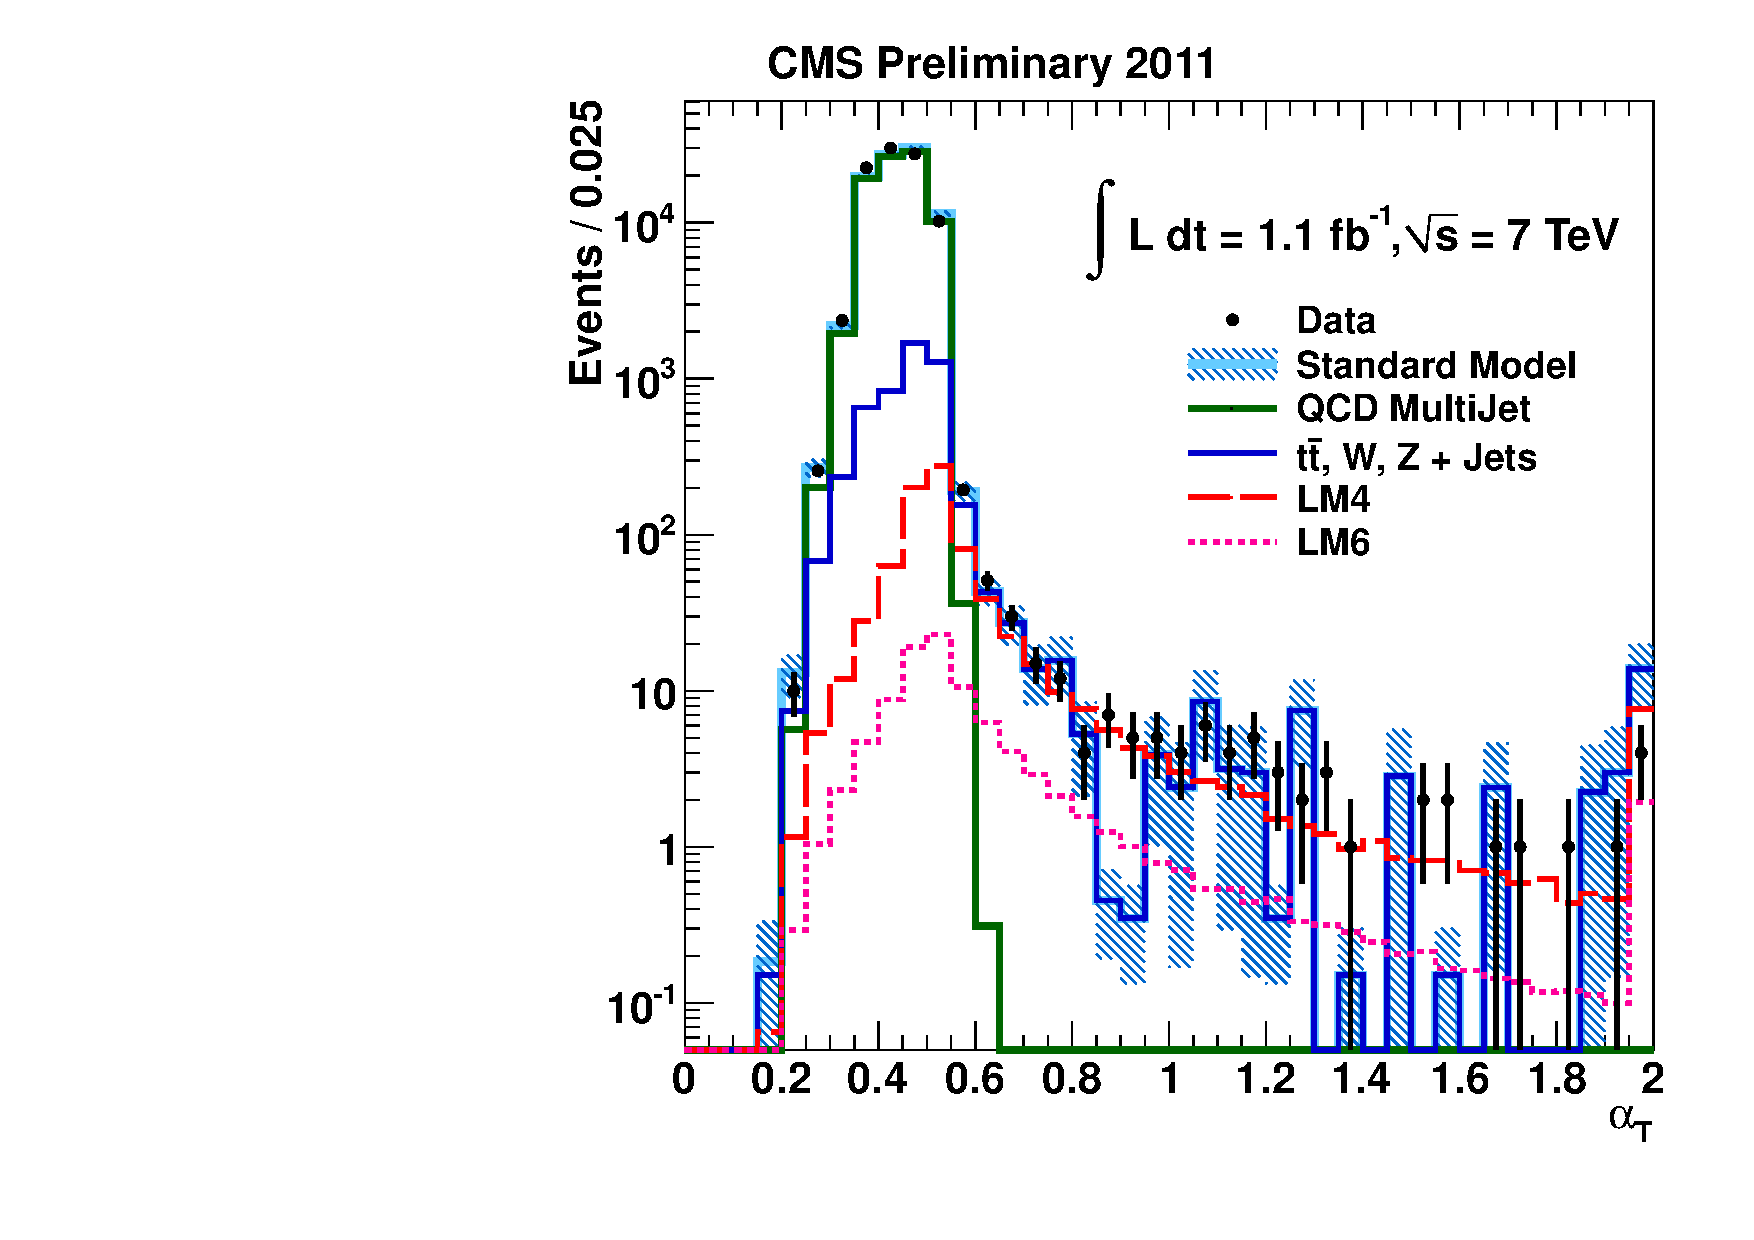
\includegraphics[width=0.40\textwidth]{Figures/Analysis/PAS/AlphaT_all.pdf}
}
\hspace{0.3cm}
  \subfigure[Comparison of the $\alpha_{T}$ distribution highlighting the agreement on the sharply falling edge between Data and Monte Carlo for the hadronic selection, in the region $H_{T}$ $\geq$ 375 GeV.]{\label{fig:figures_AlphaT_Zoomed_all}
          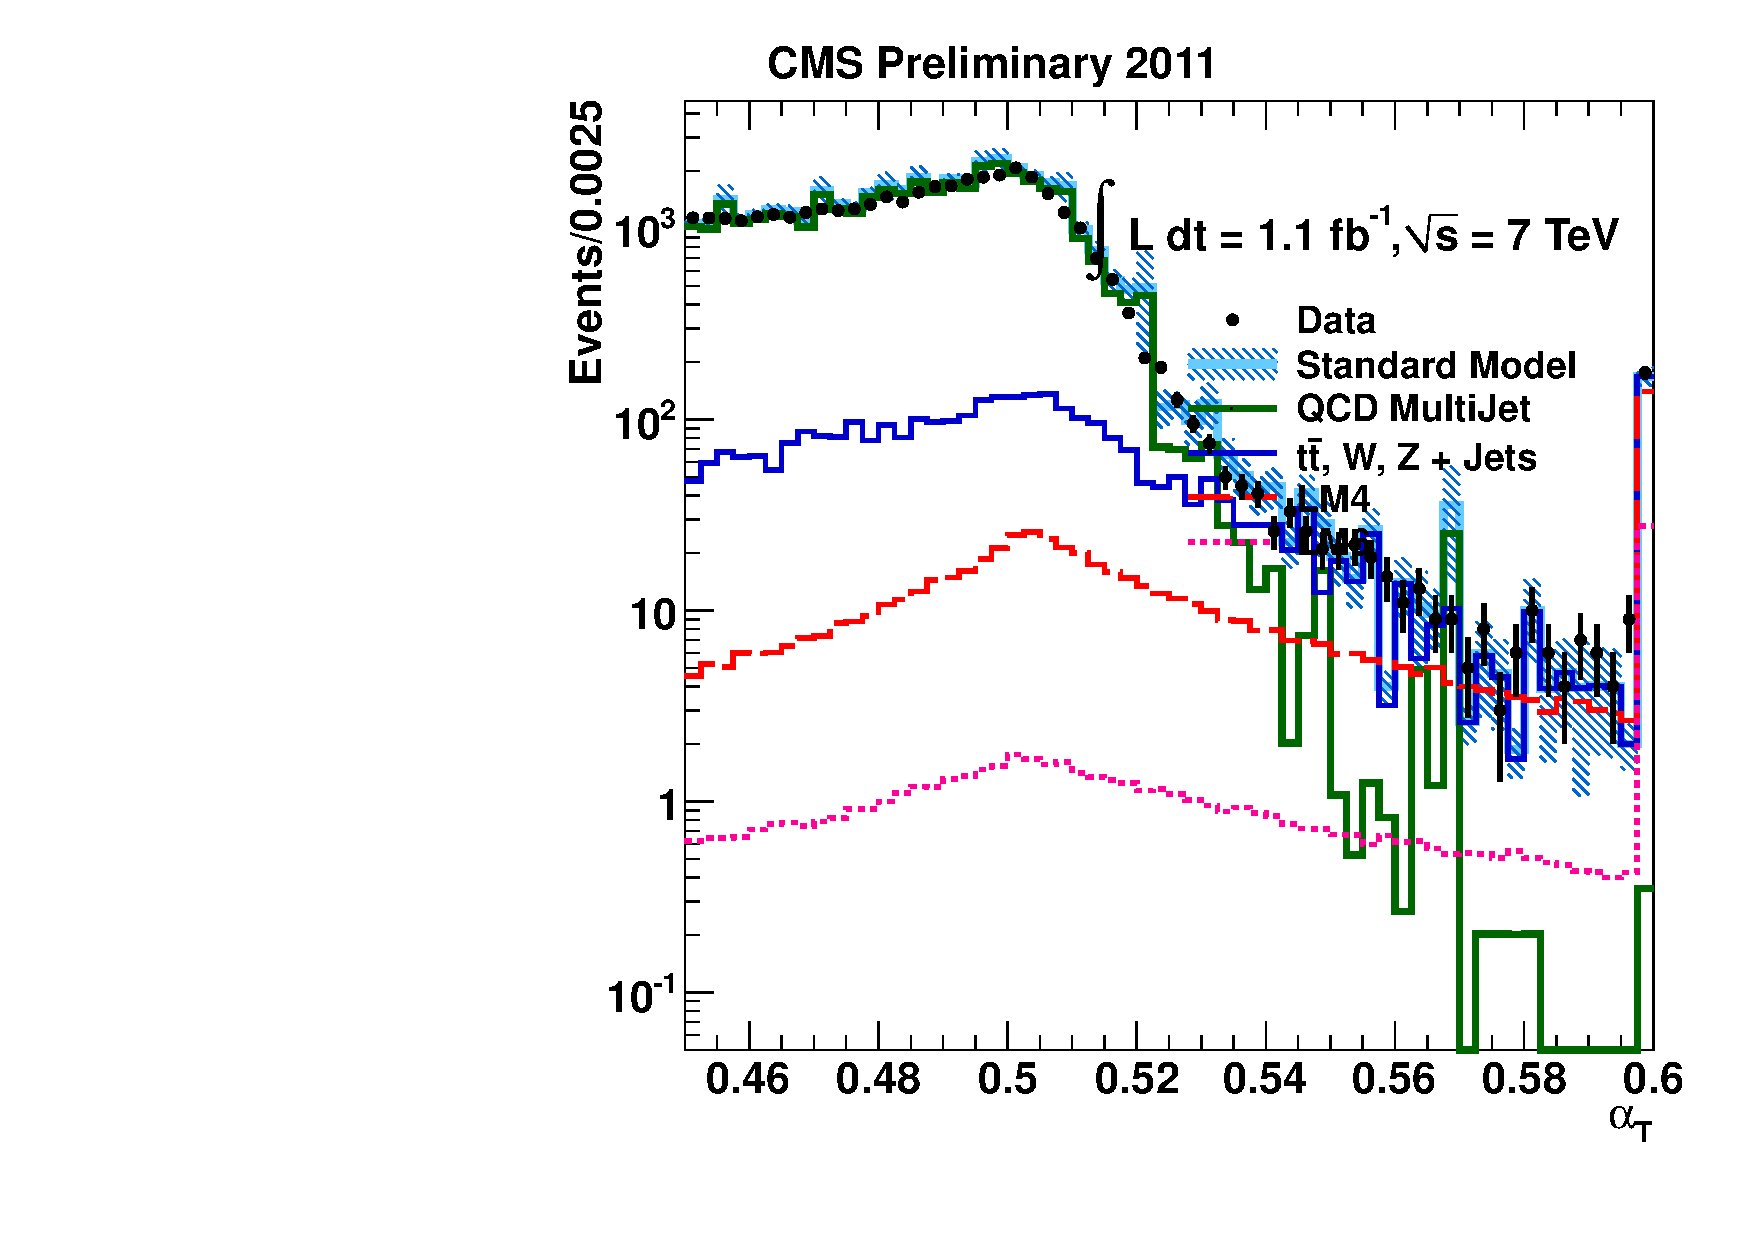
\includegraphics[width=0.40\textwidth]{Figures/Analysis/PAS/AlphaT_Zoomed_all.pdf}
     }
    \caption{Comparisons of 1.1 \fb 2011 7TeV CMS Data and equivalently weighted Monte-Carlo in basic kinematic quantities prior to the $\alpha_{T}$ selection cut.}
\end{figure}
\begin{figure}[h]
    \centering
     \subfigure[$\Delta \Phi^{*}$ distribution after $\alpha_{T}$ selection.]{
          \label{fig:BiasedDeltaPhi_after_alphaT_55_all}
          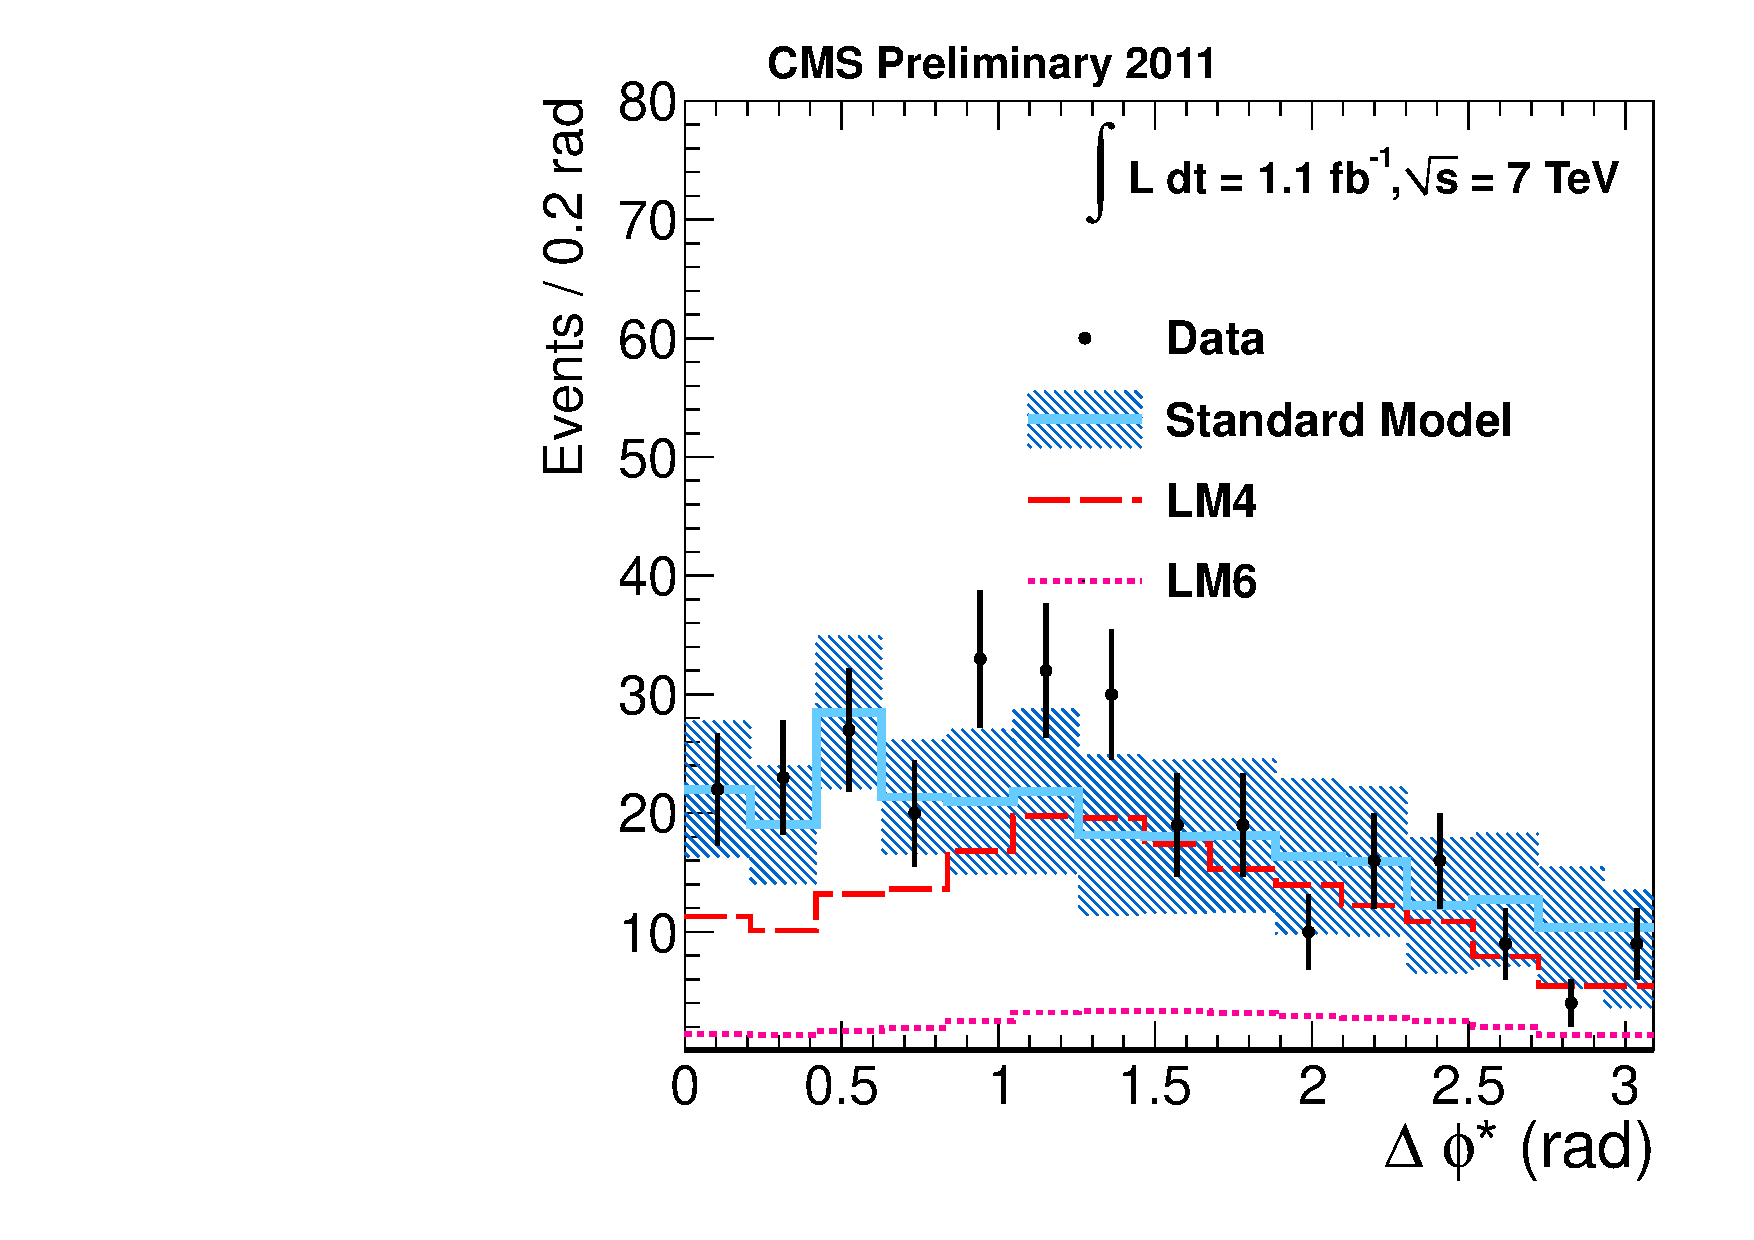
\includegraphics[width=0.46\textwidth]{Figures/Analysis/PAS/BiasedDeltaPhi_after_alphaT_55_all.pdf}
     }
\hspace{0.3cm}
    \subfigure[The effective mass distribution, $M_{\rm eff}$ = $H_{T}$ +
    MHT, of the events passing the $\alpha_{T}$ selection.]{
          \label{fig:EffectiveMass_after_alphaT_55_all}
          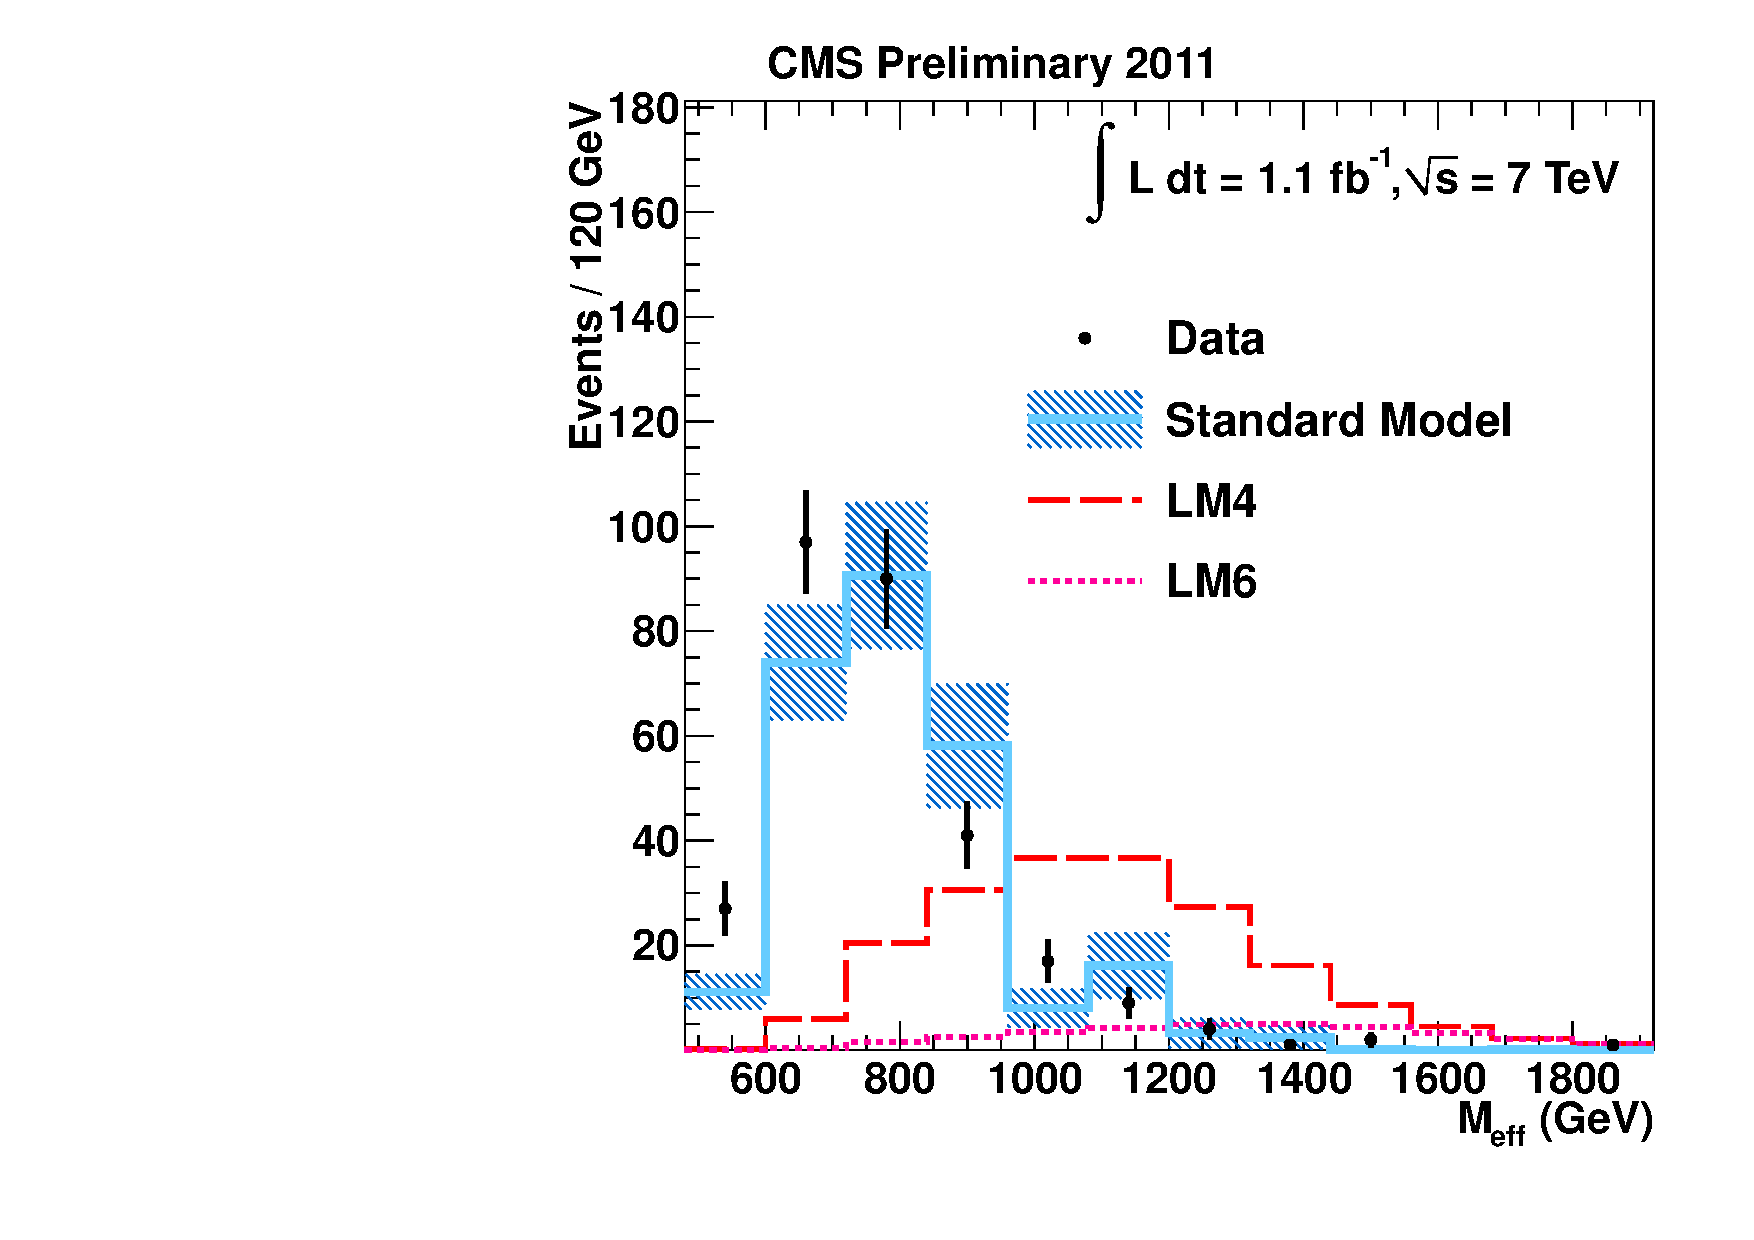
\includegraphics[width=0.46\textwidth]{Figures/Analysis/PAS/EffectiveMass_after_alphaT_55_all.pdf}
     }
    \newline
    \subfigure[Jet multiplicity after $\alpha_{T}$ selection.]{
          \label{fig:JetMultiplicityAfterAlphaT_all}
          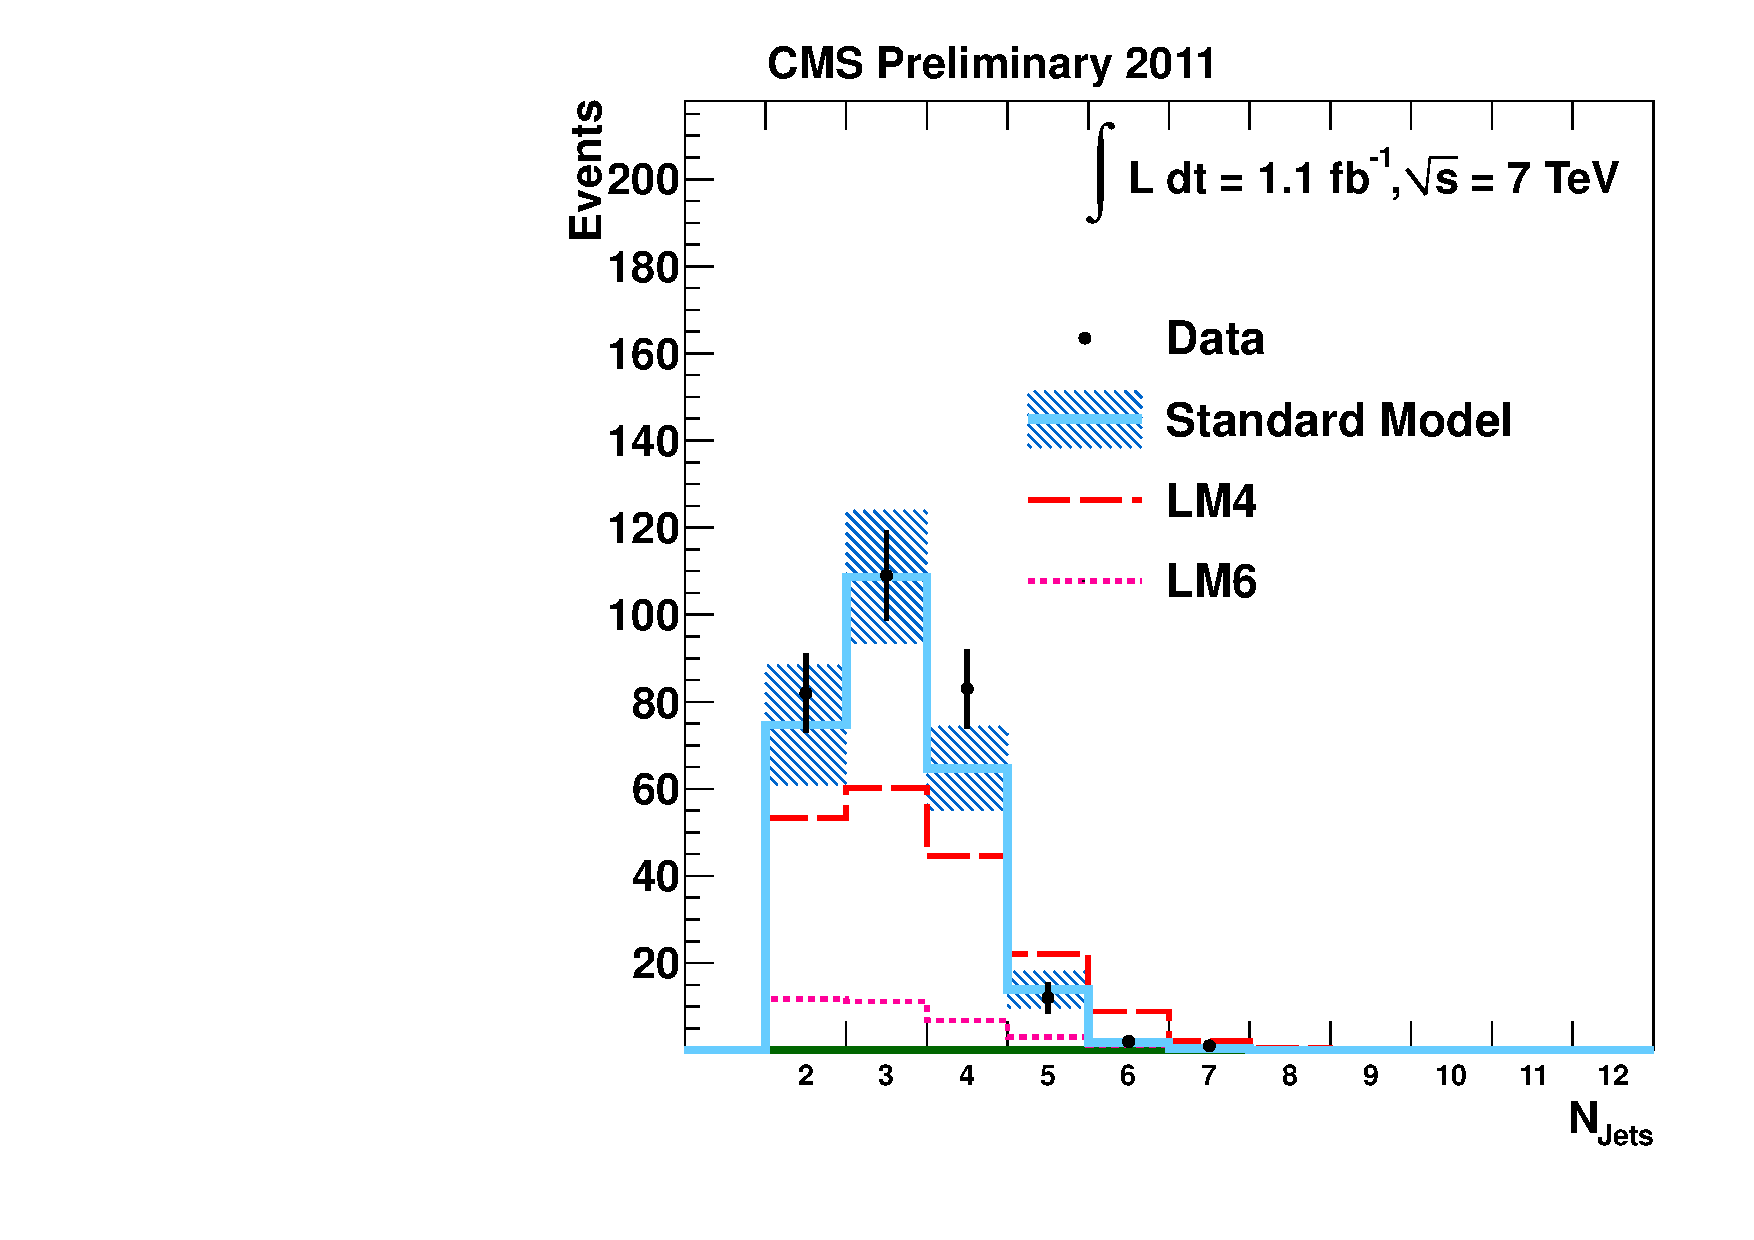
\includegraphics[width=0.46\textwidth]{Figures/Analysis/PAS/JetMultiplicityAfterAlphaT_all.pdf}
     }
\caption{Comparisons of 1.1 \fb 2011 7TeV CMS Data and equivalently weighted Monte-Carlo in basic kinematic quantities after the $\alpha_{T}$ selection cut.}
\end{figure}

\subsection{Dependence of $R_{\alpha_{T}}$ on $H_{T}$}




\begin{figure}[h]
  \begin{center}
    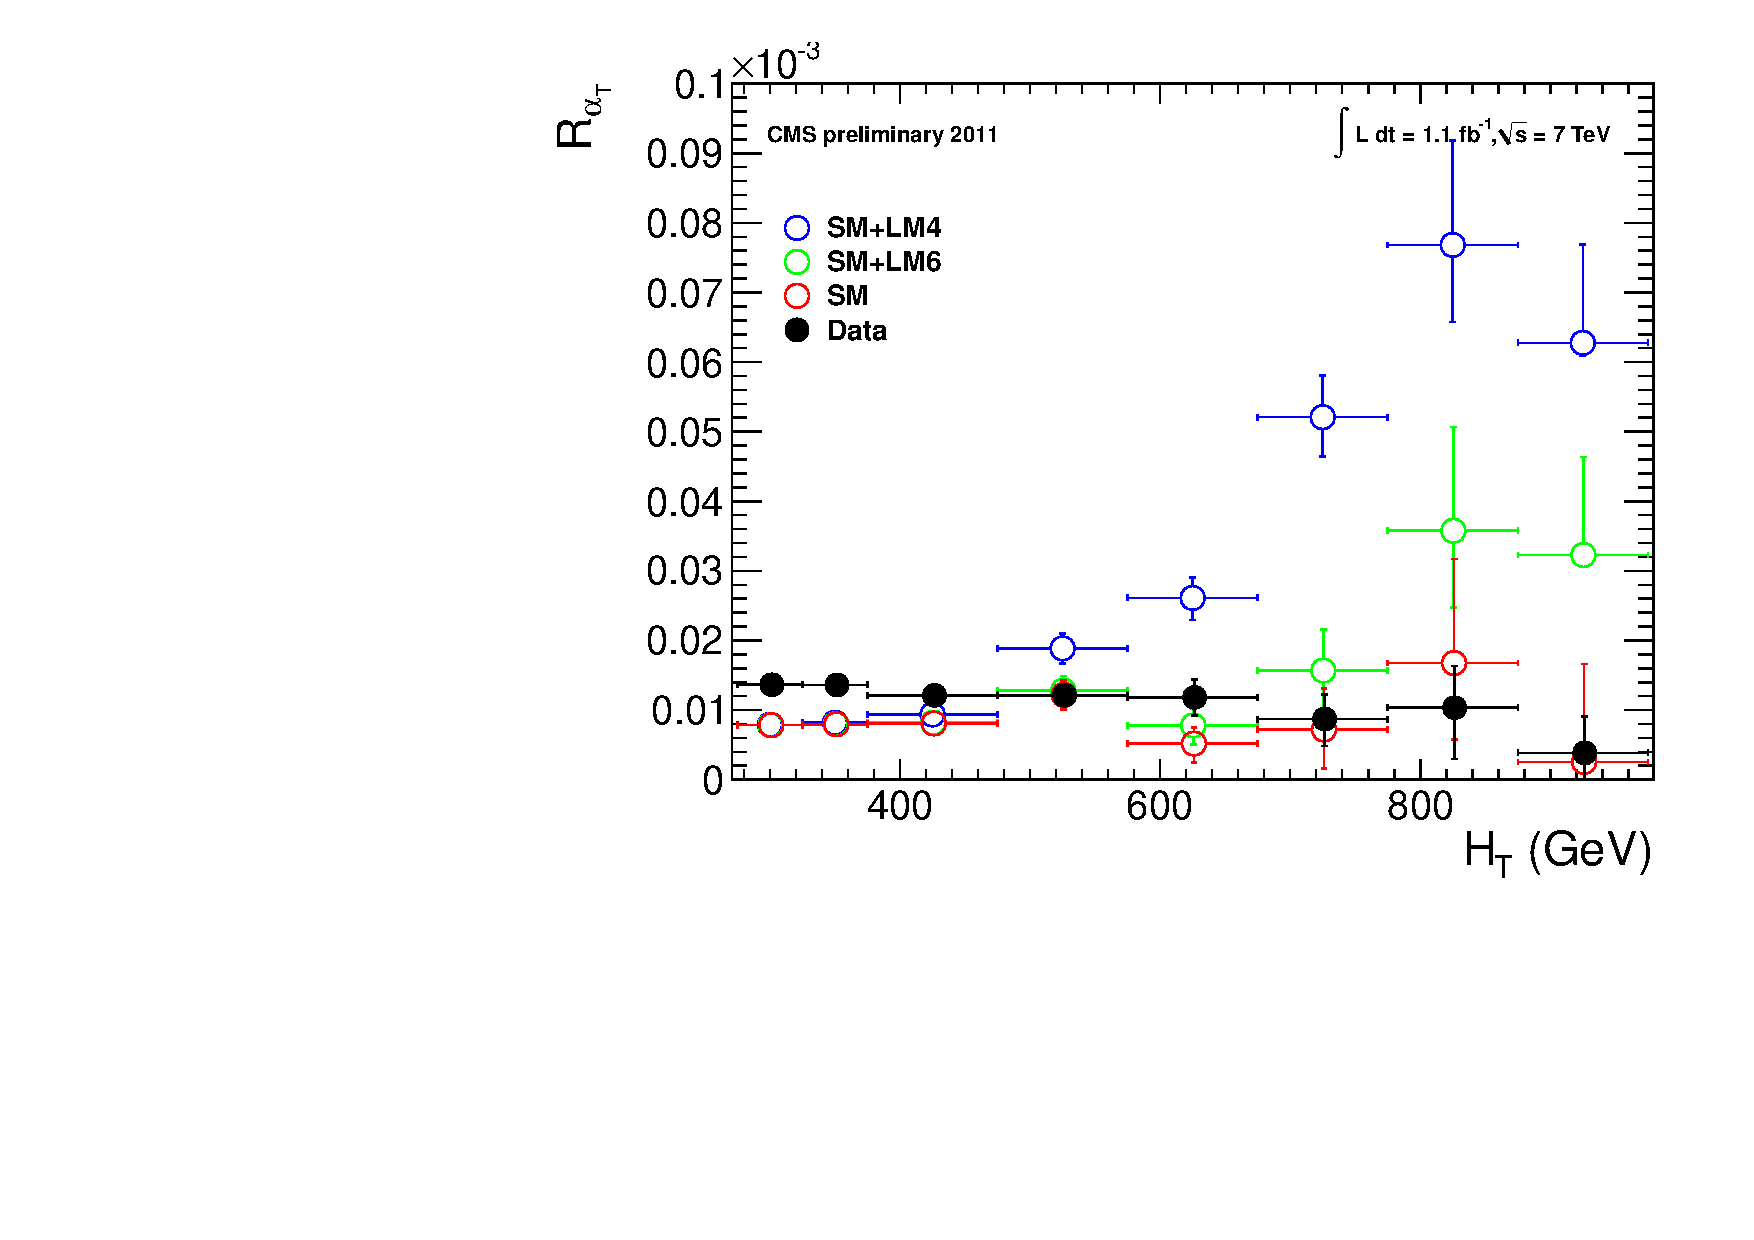
\includegraphics[width = 0.48\textwidth]{Figures/Analysis/PAS/Ratio_Multi2Incl_AlphaT55.pdf}
    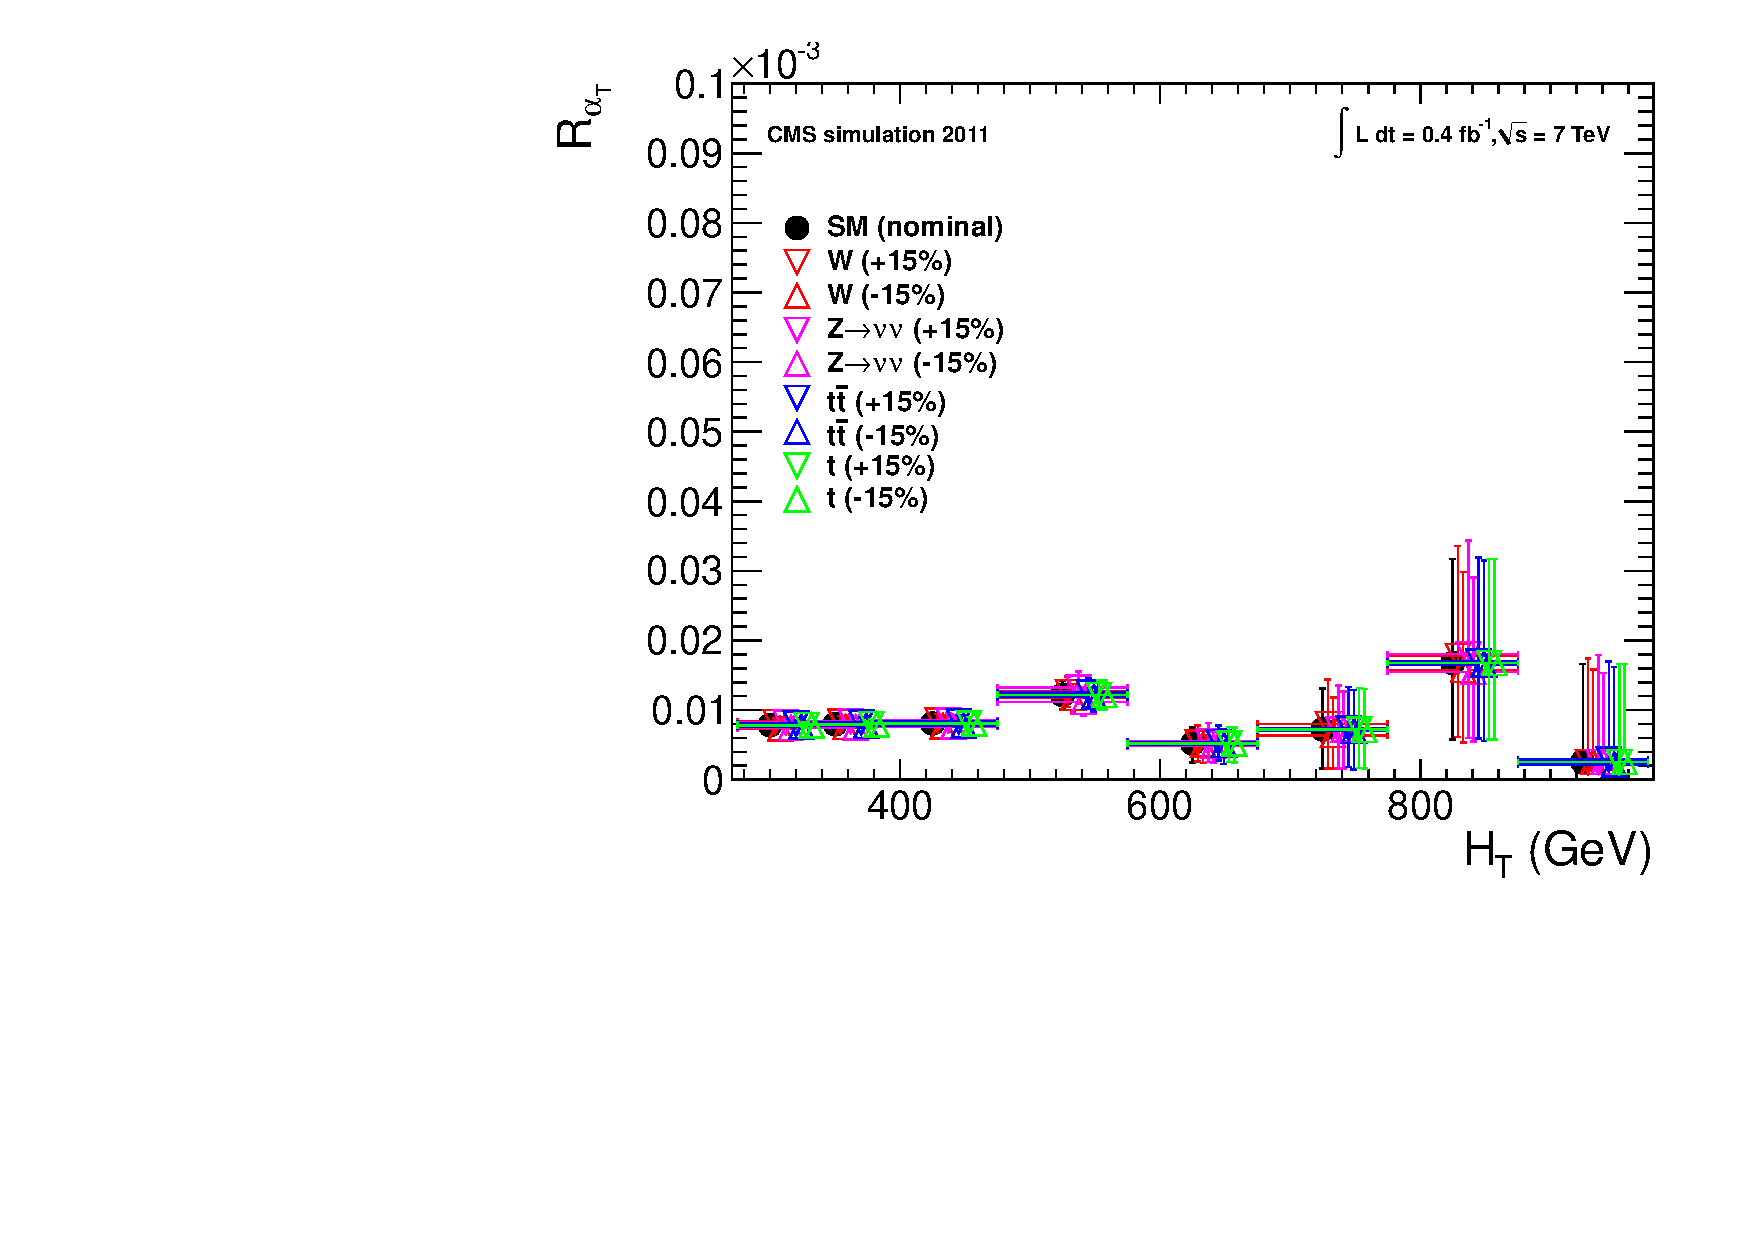
\includegraphics[width = 0.48\textwidth]{Figures/Analysis/PAS/Syst_Multi2Incl_AlphaT55.pdf}
    \caption{\label{fig:rat_vs_ht} (Left) The dependence of \RaT on
      \HT for events with N$_{\mathrm{jet}} \geq 2$. (Right) Dependence of rat on
      \HT when varying the effective cross-section of the four major
      EWK background components individually by $\pm$15\%. (Markers
      are artificially offset for clarity.)  }
  \end{center}
\end{figure}






\section{Data-Driven Background Estimation}
\subsection{Total background prediction}
\subsection{Estimating EWK background using high $p_{T}$ using W+Jets events}
\begin{figure}[h]
\begin{center}
\subfigure[\label{fig:muon_beforeat_mupt}]{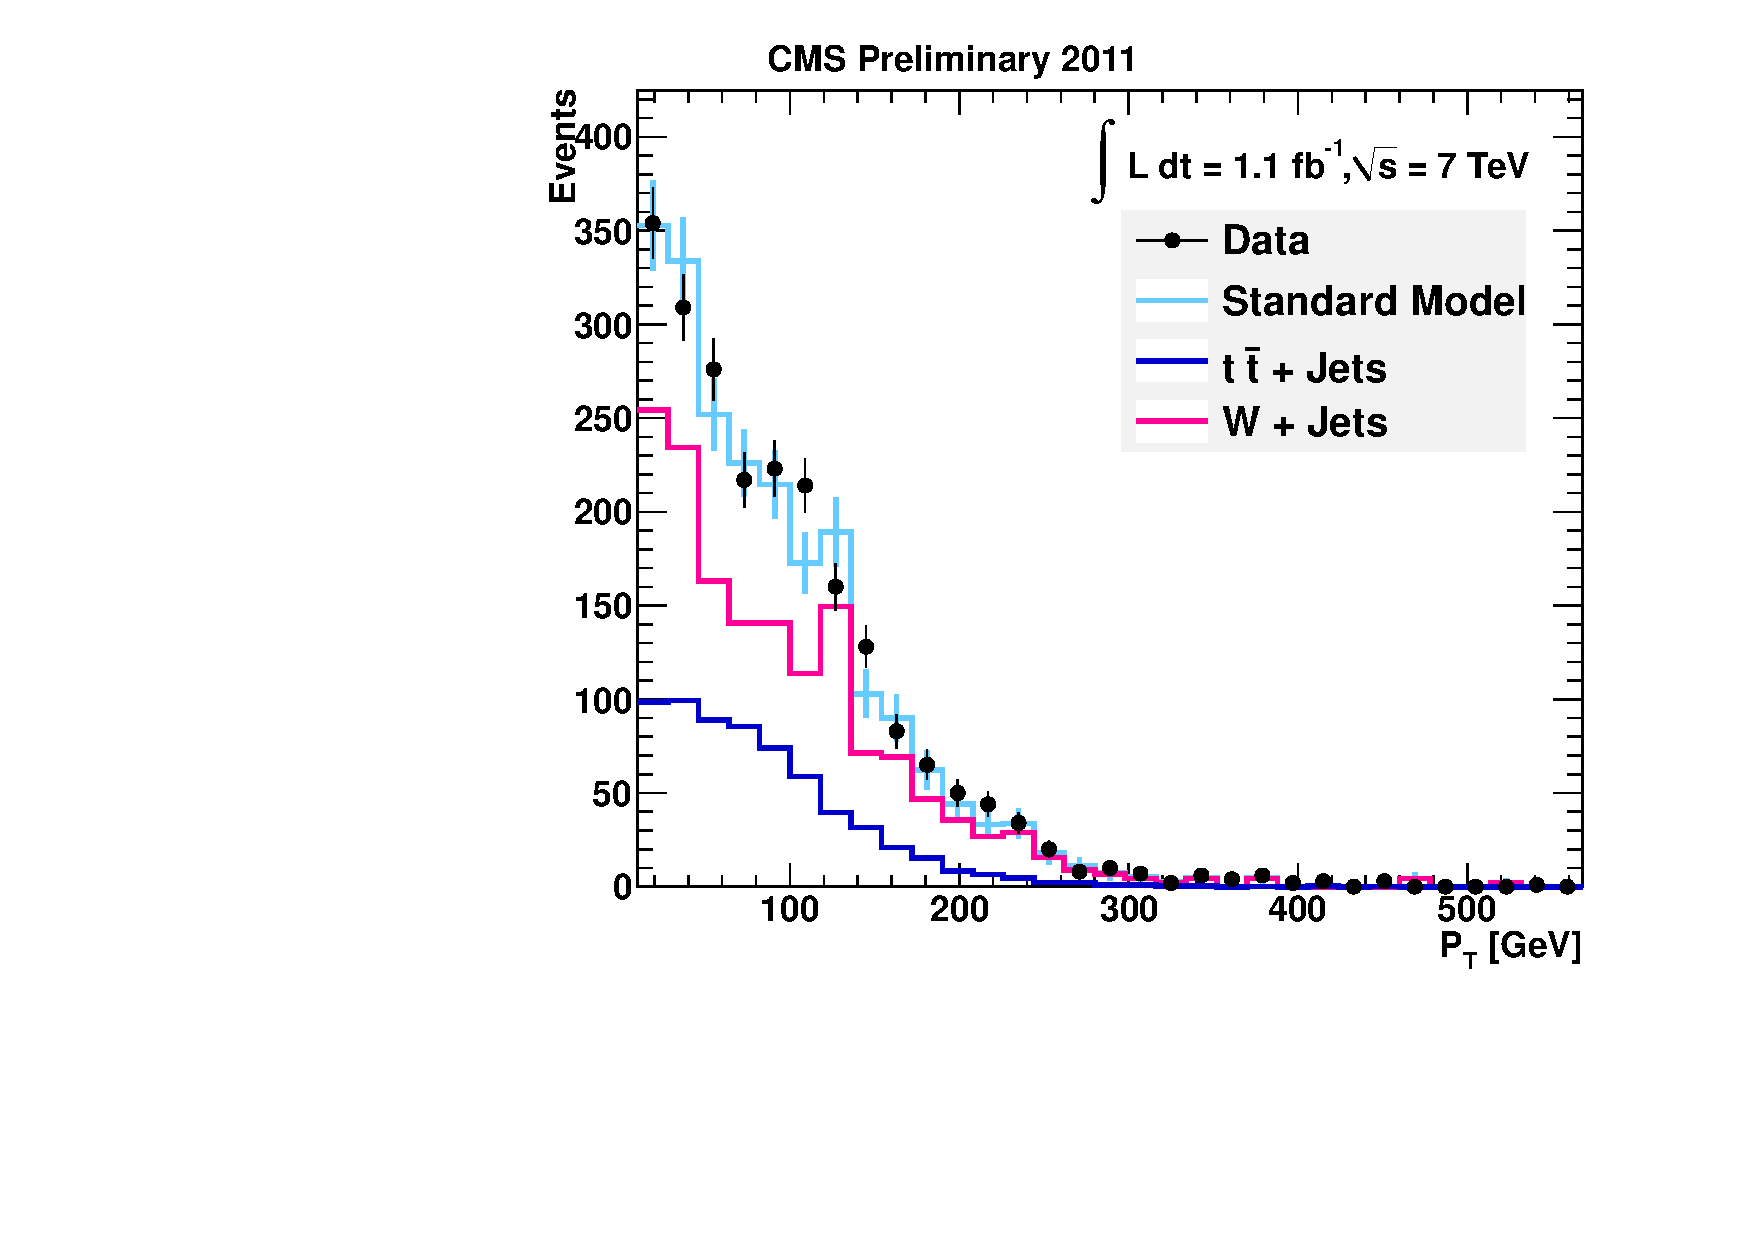
\includegraphics[width=0.45\textwidth, angle=0]{Figures/Analysis/PAS/muon_plots/spring11NoLogYMuPtMuonControl_beforeaT.pdf}}
\subfigure[\label{fig:muon_beforeat_njet}]{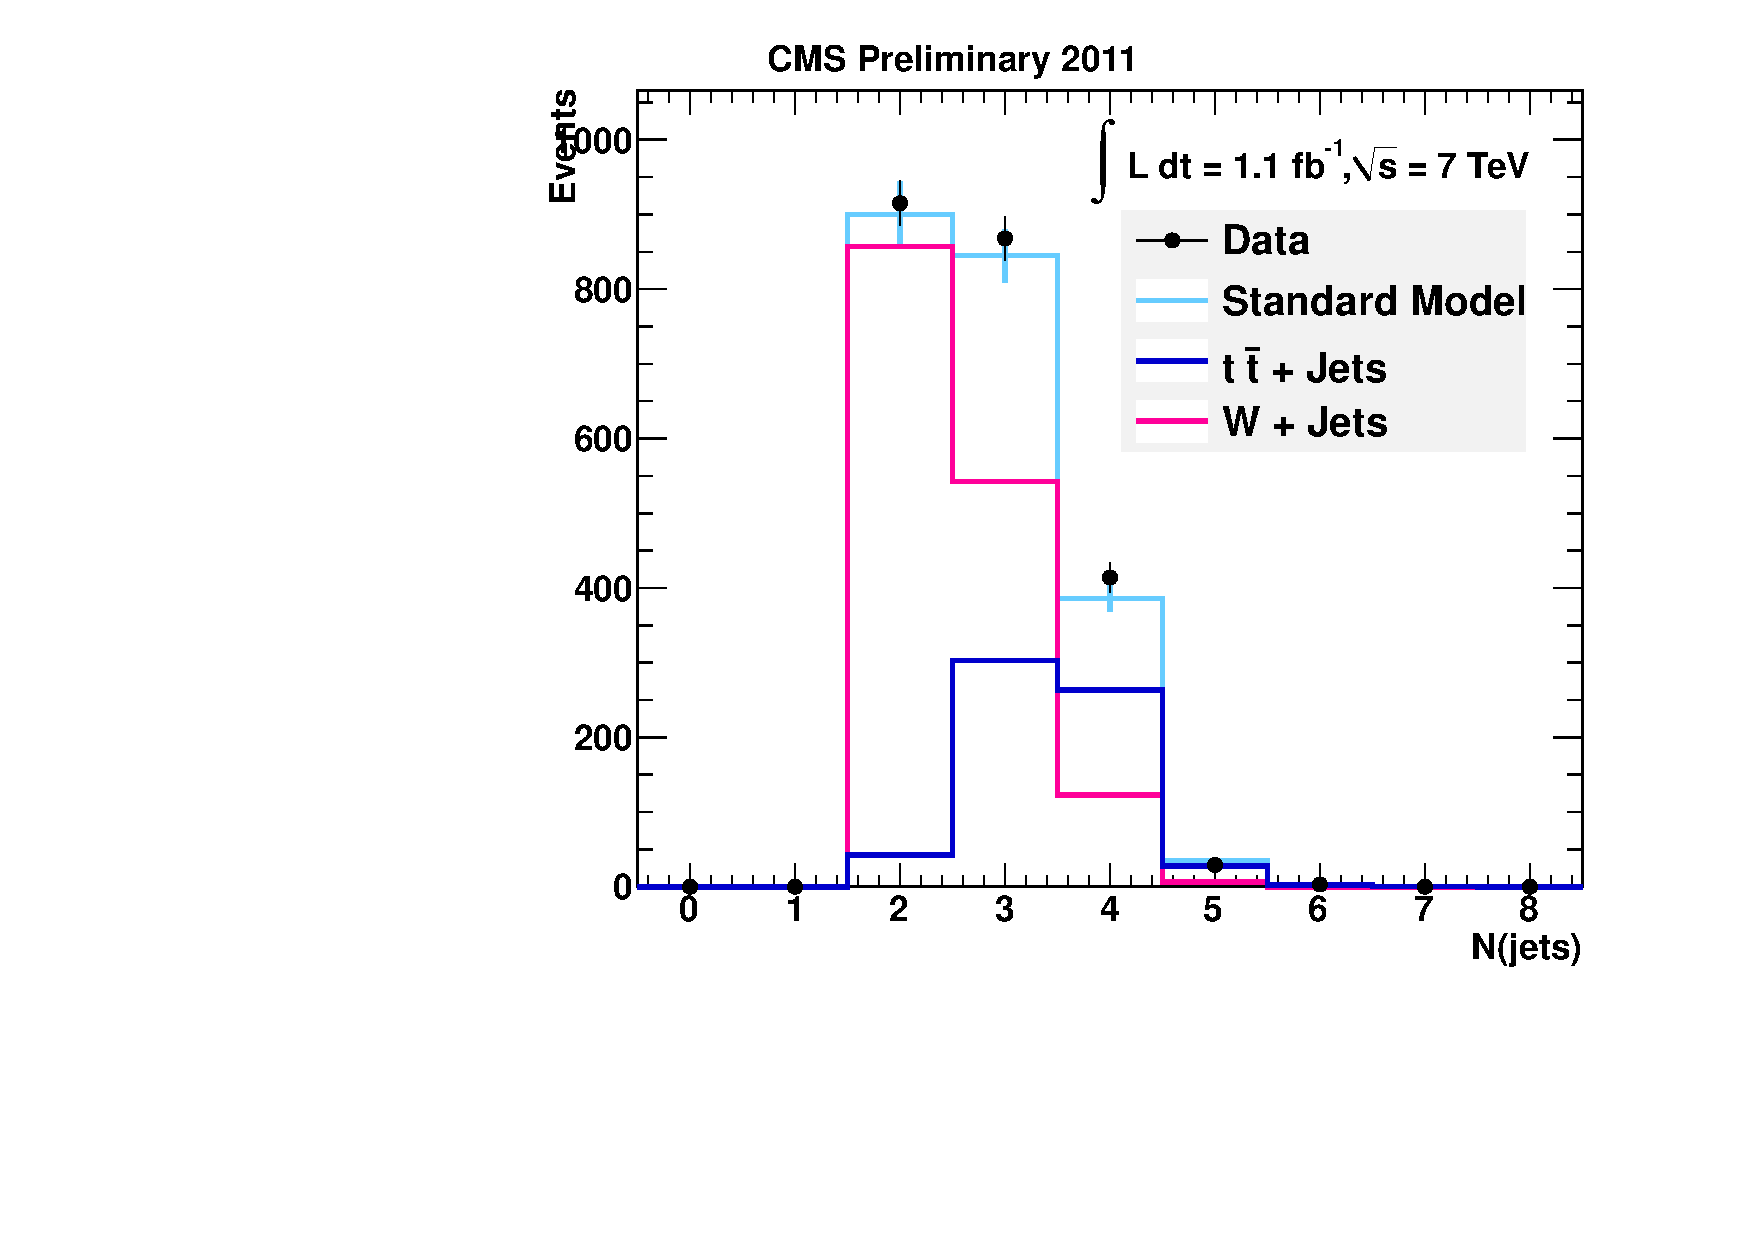
\includegraphics[width=0.45\textwidth, angle=0]{Figures/Analysis/PAS/muon_plots/spring11NoLogYnJetMuonControl_beforeaT.pdf}}
\newline
\subfigure[\label{fig:muon_beforeat_at}]{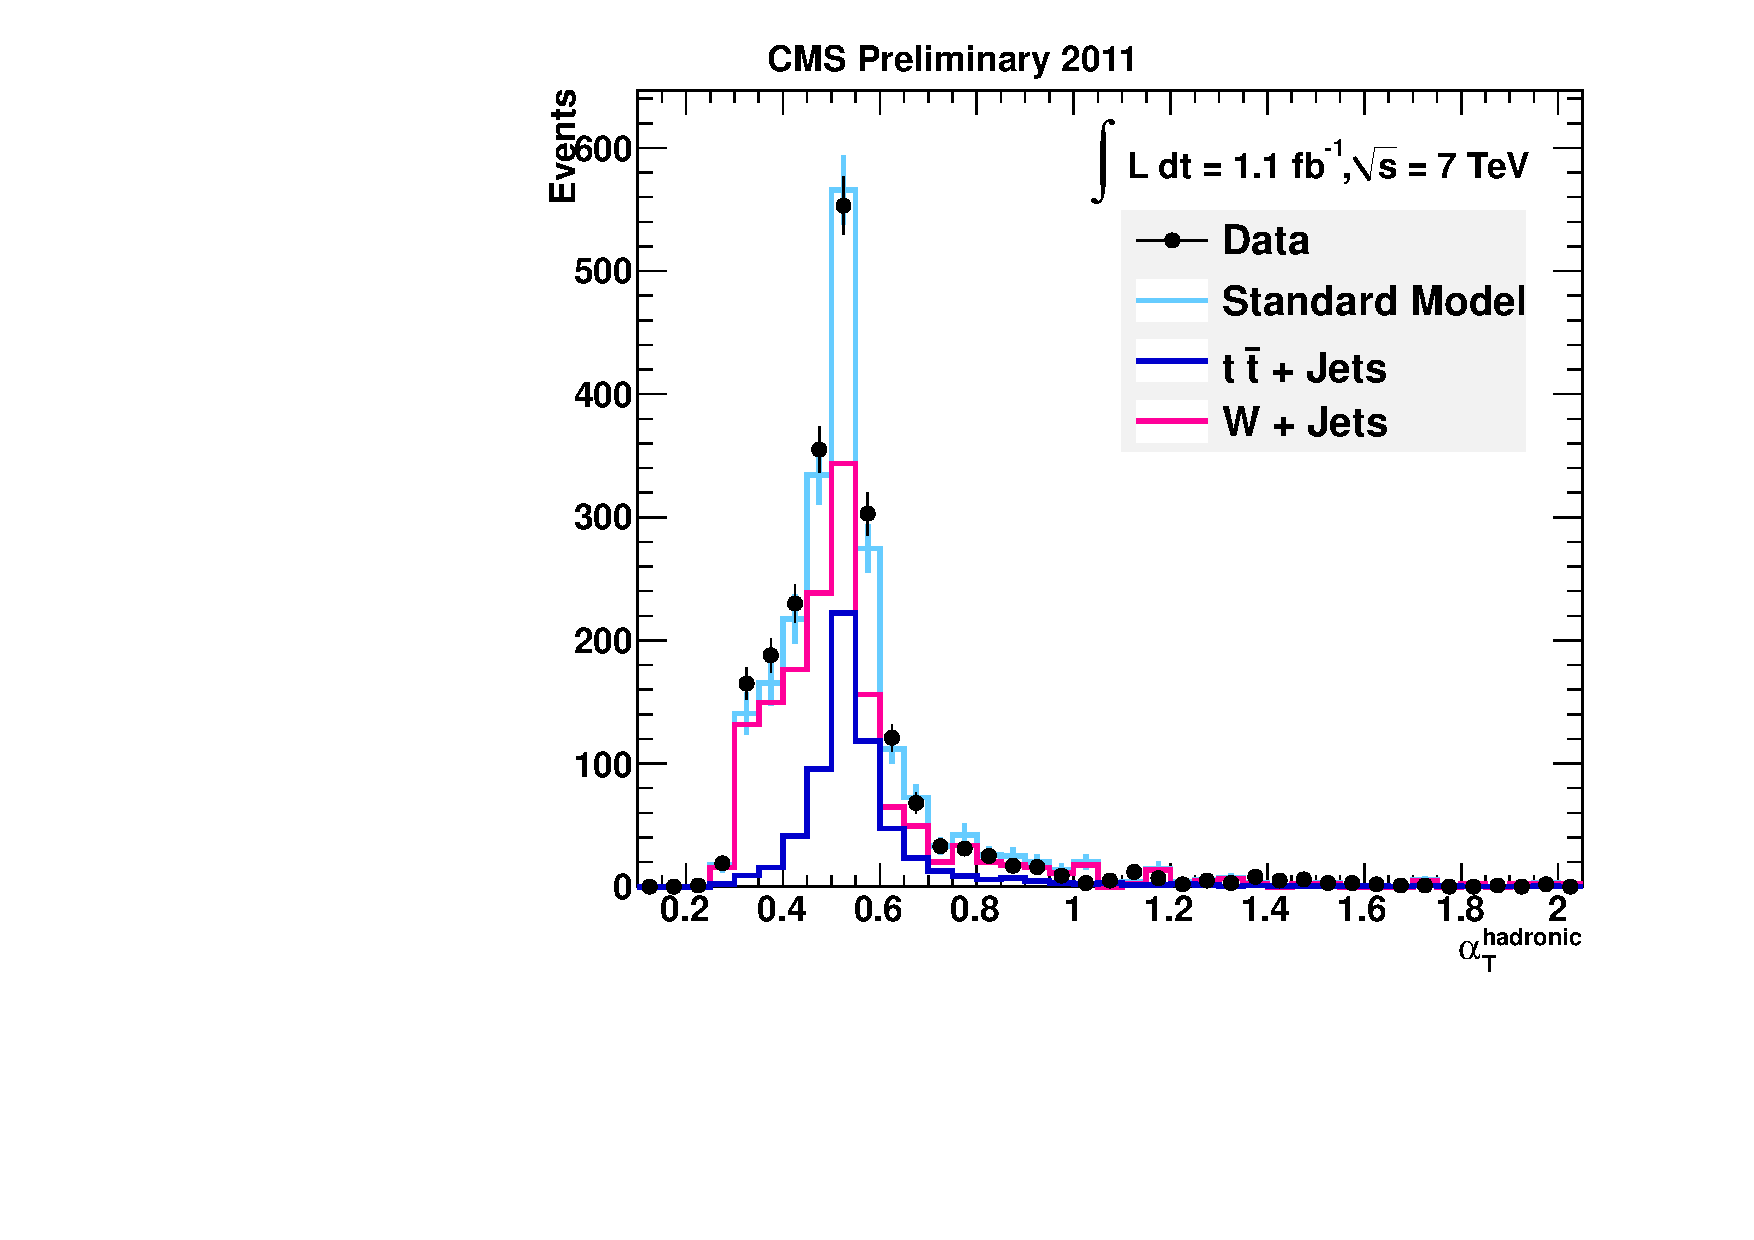
\includegraphics[width=0.45\textwidth, angle=0]{Figures/Analysis/PAS/muon_plots/spring11NoLogYaT_HMuonControl_beforeaT.pdf}}
\subfigure[\label{fig:muon_beforeat_ht}]{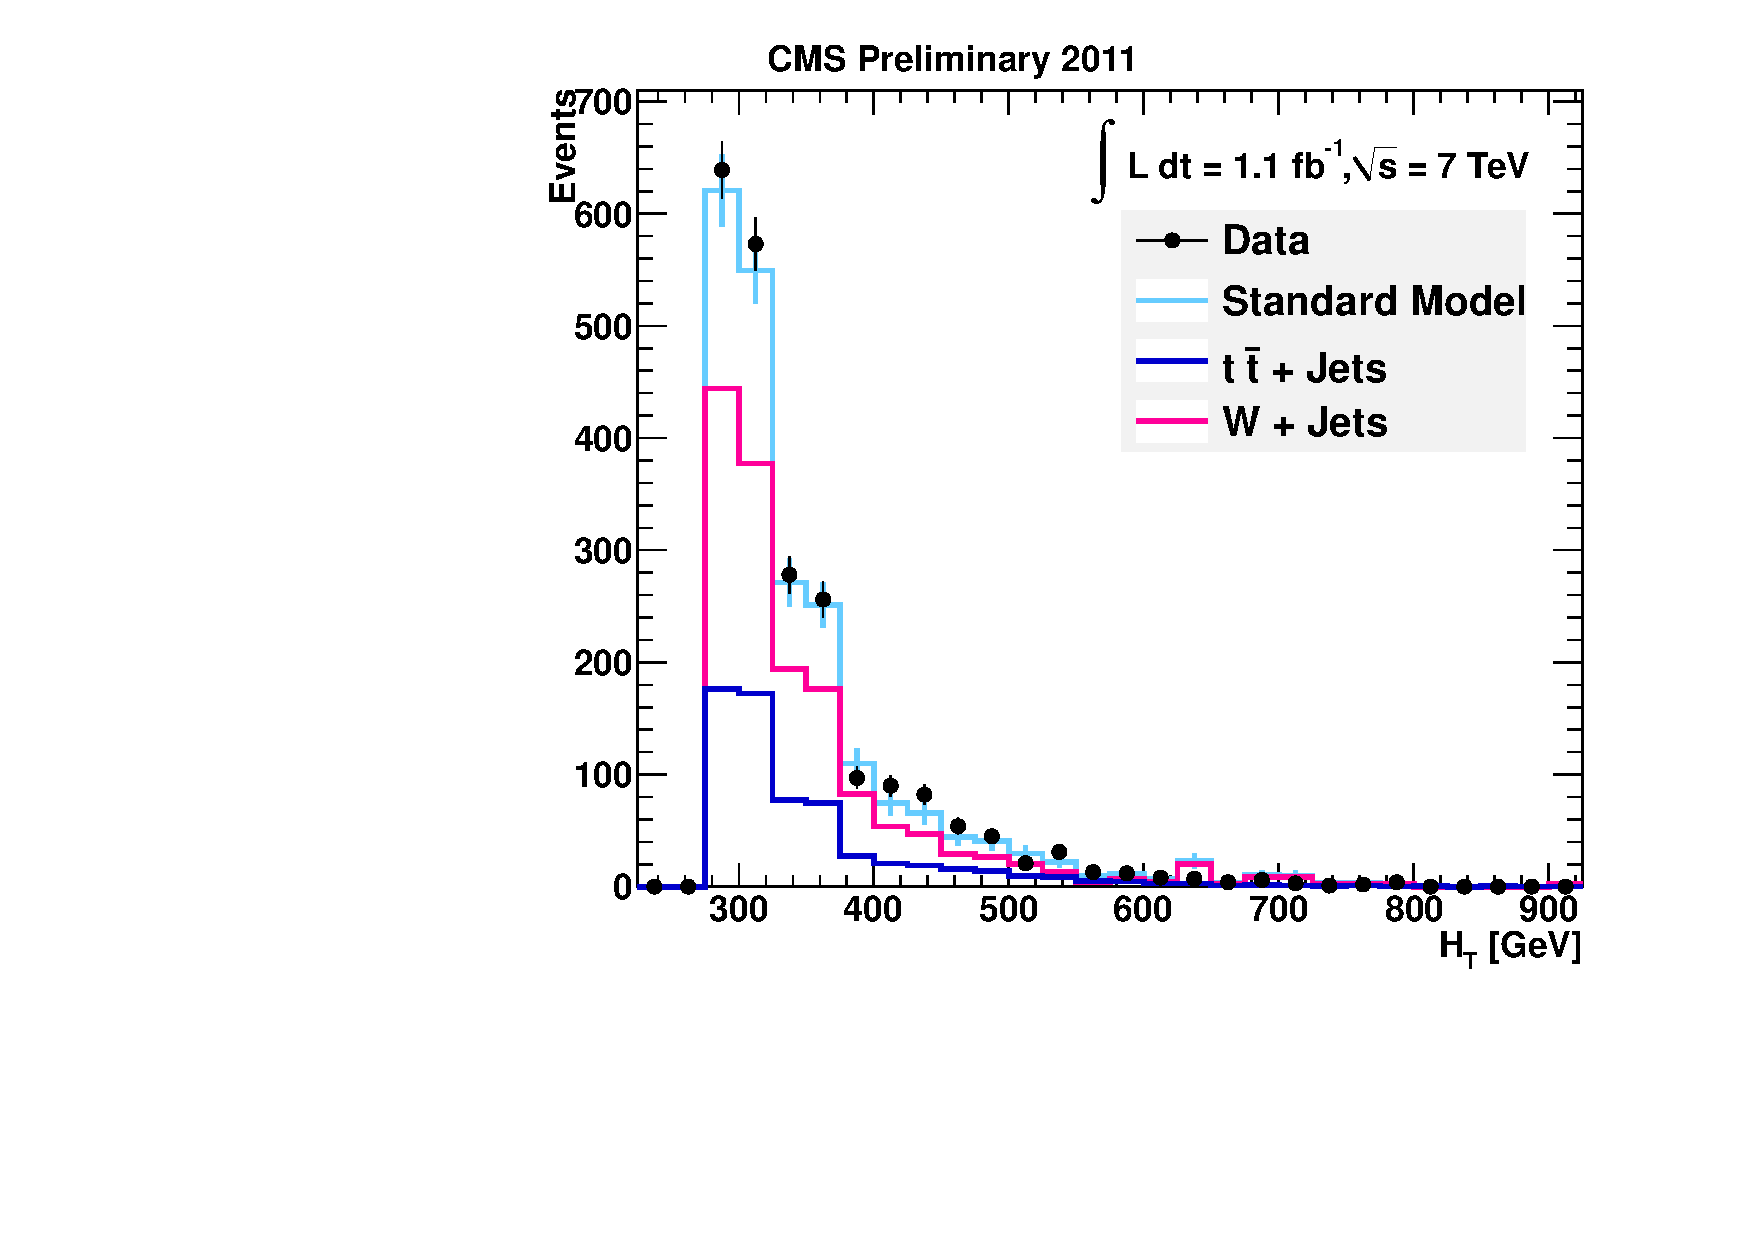
\includegraphics[width=0.45\textwidth, angle=0]{Figures/Analysis/PAS/muon_plots/spring11NoLogYHTMuonControl_beforeaT.pdf}}
\newline
\subfigure[\label{fig:muon_beforeat_MuIso}]{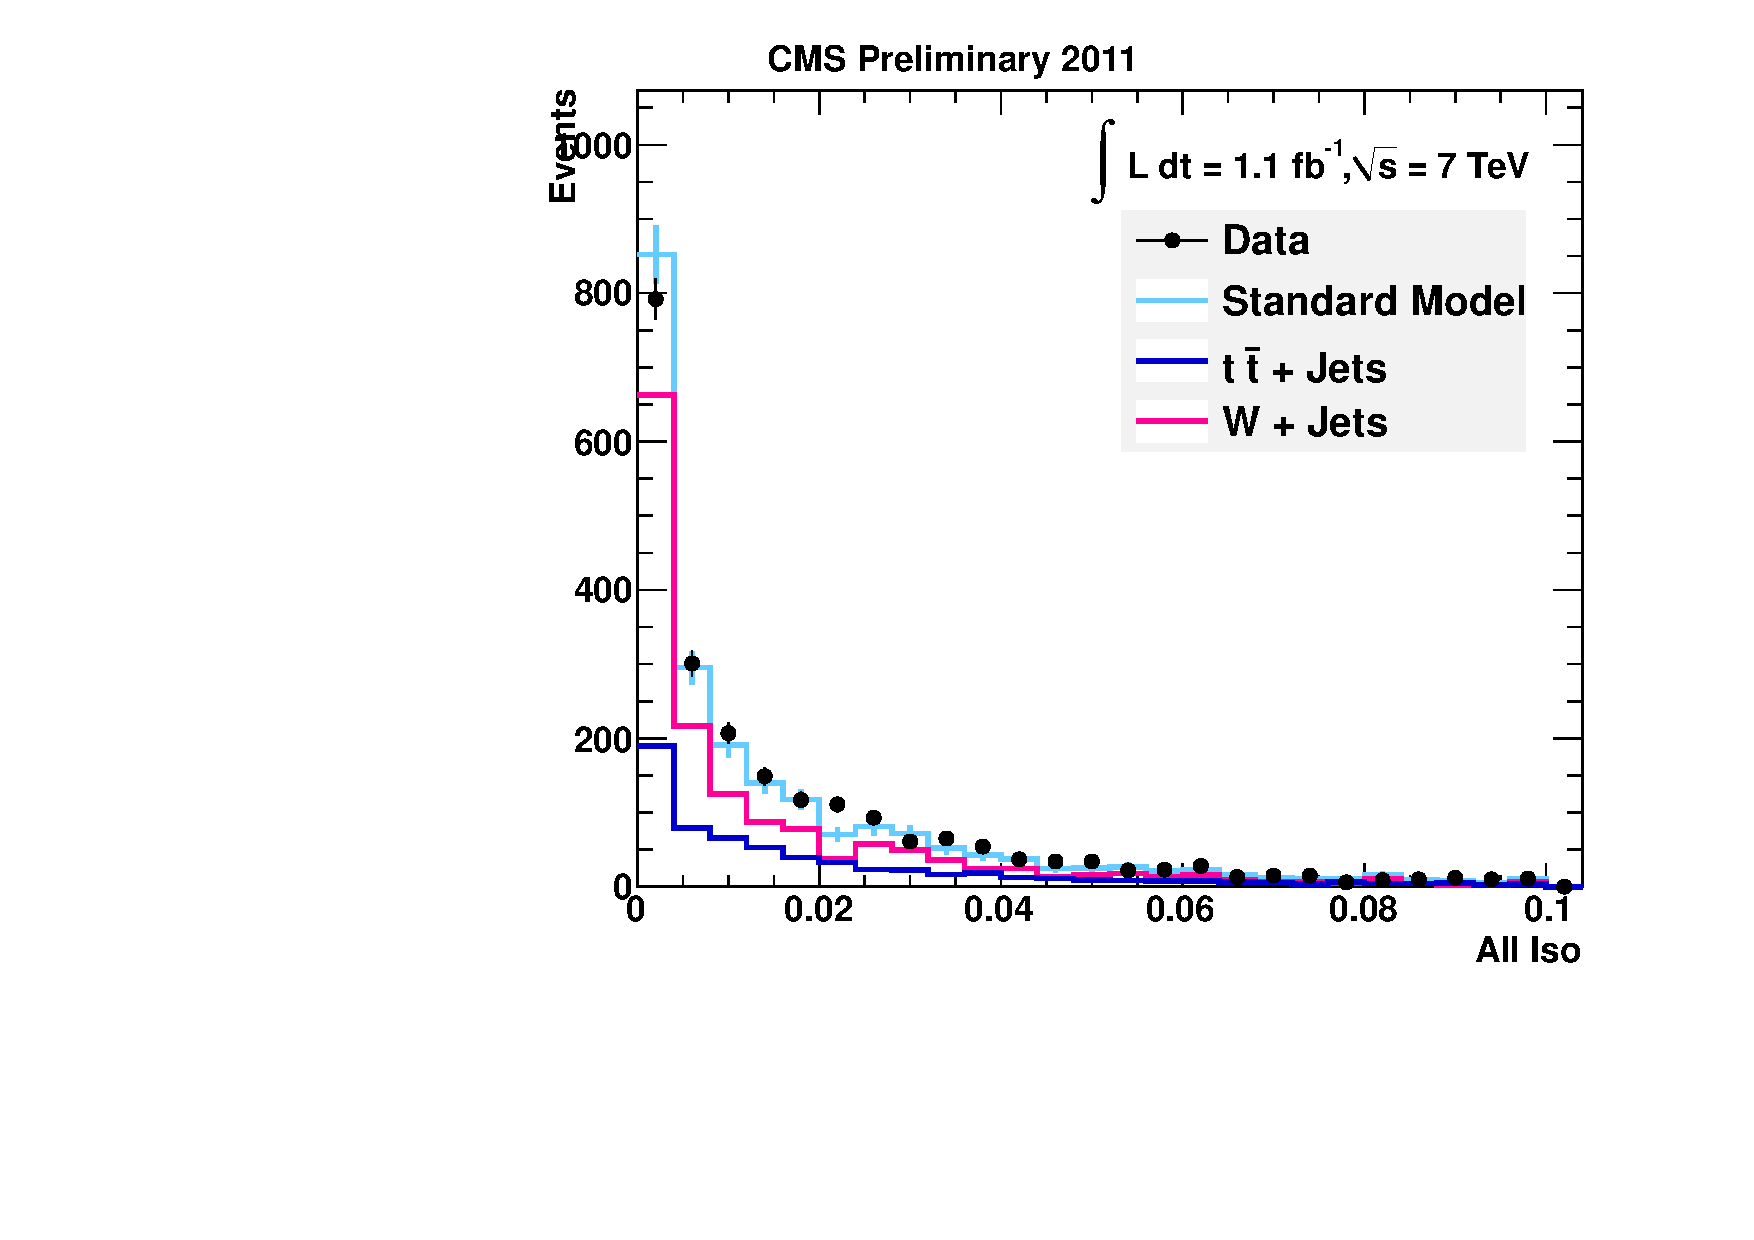
\includegraphics[width=0.45\textwidth, angle=0]{Figures/Analysis/PAS/muon_plots/spring11NoLogYMuCsoMuonControl_beforeaT.pdf}}
\subfigure[\label{fig:muon_beforeat_mt}]{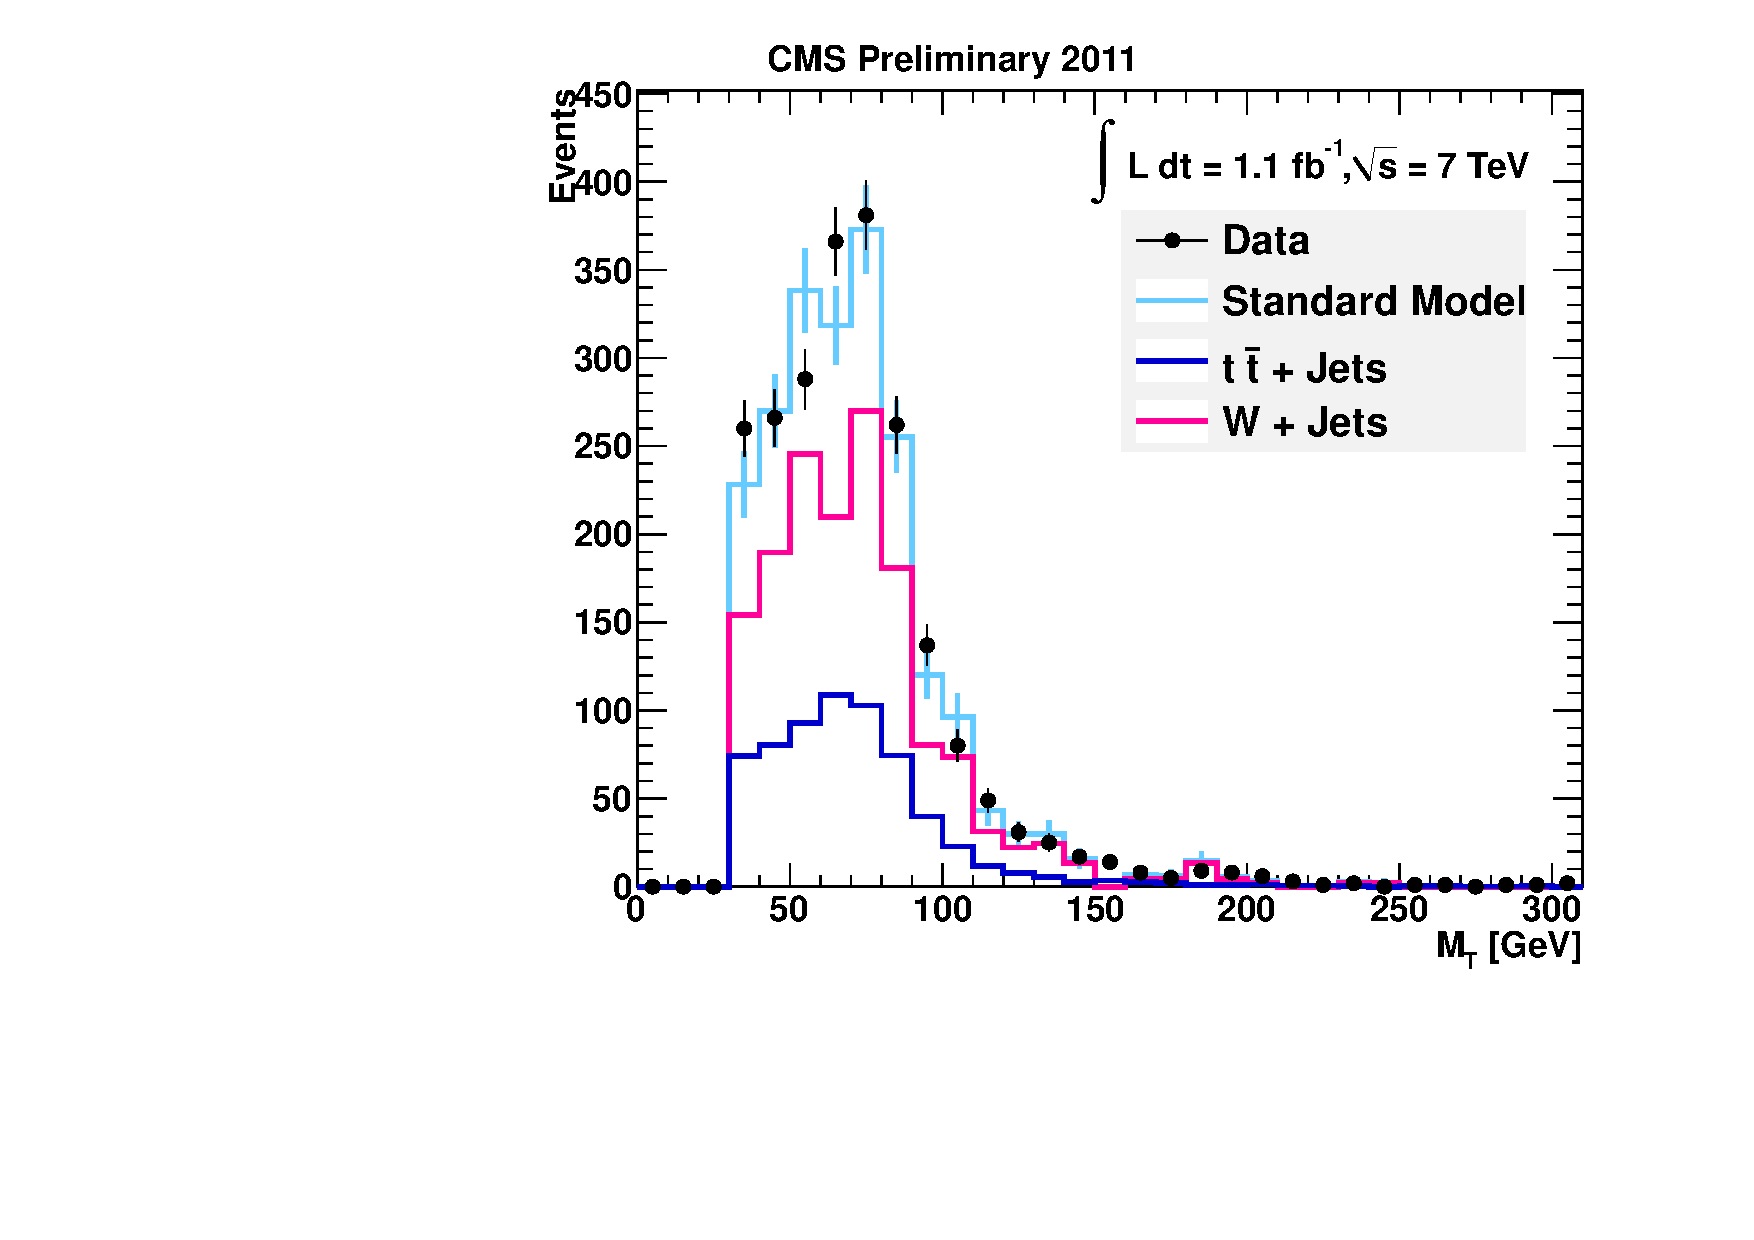
\includegraphics[width=0.45\textwidth, angle=0]{Figures/Analysis/PAS/muon_plots/spring11NoLogYMTMuonControl_beforeaT.pdf}}

\caption{\label{fig:muonplots_beforeat} Data - Monte Carlo comparisons
  for the muon control selection before the $\alpha_{T} > 0.55$ cut is
  applied, shown for (a) $\alpha_{T}$ and (b) $H_{T}$, (c) Muon  Combined Isolation and (d) $M_{T}$.
 A cut of $\mathrm{HT >}$375 GeV has been applied, to select the
 region of fixed jet thresholds.}
\label{fig:kin}
\end{center}
\end{figure}

\begin{figure}[h]
\begin{center}
\subfigure[\label{fig:muon_beforeat_mupt}]{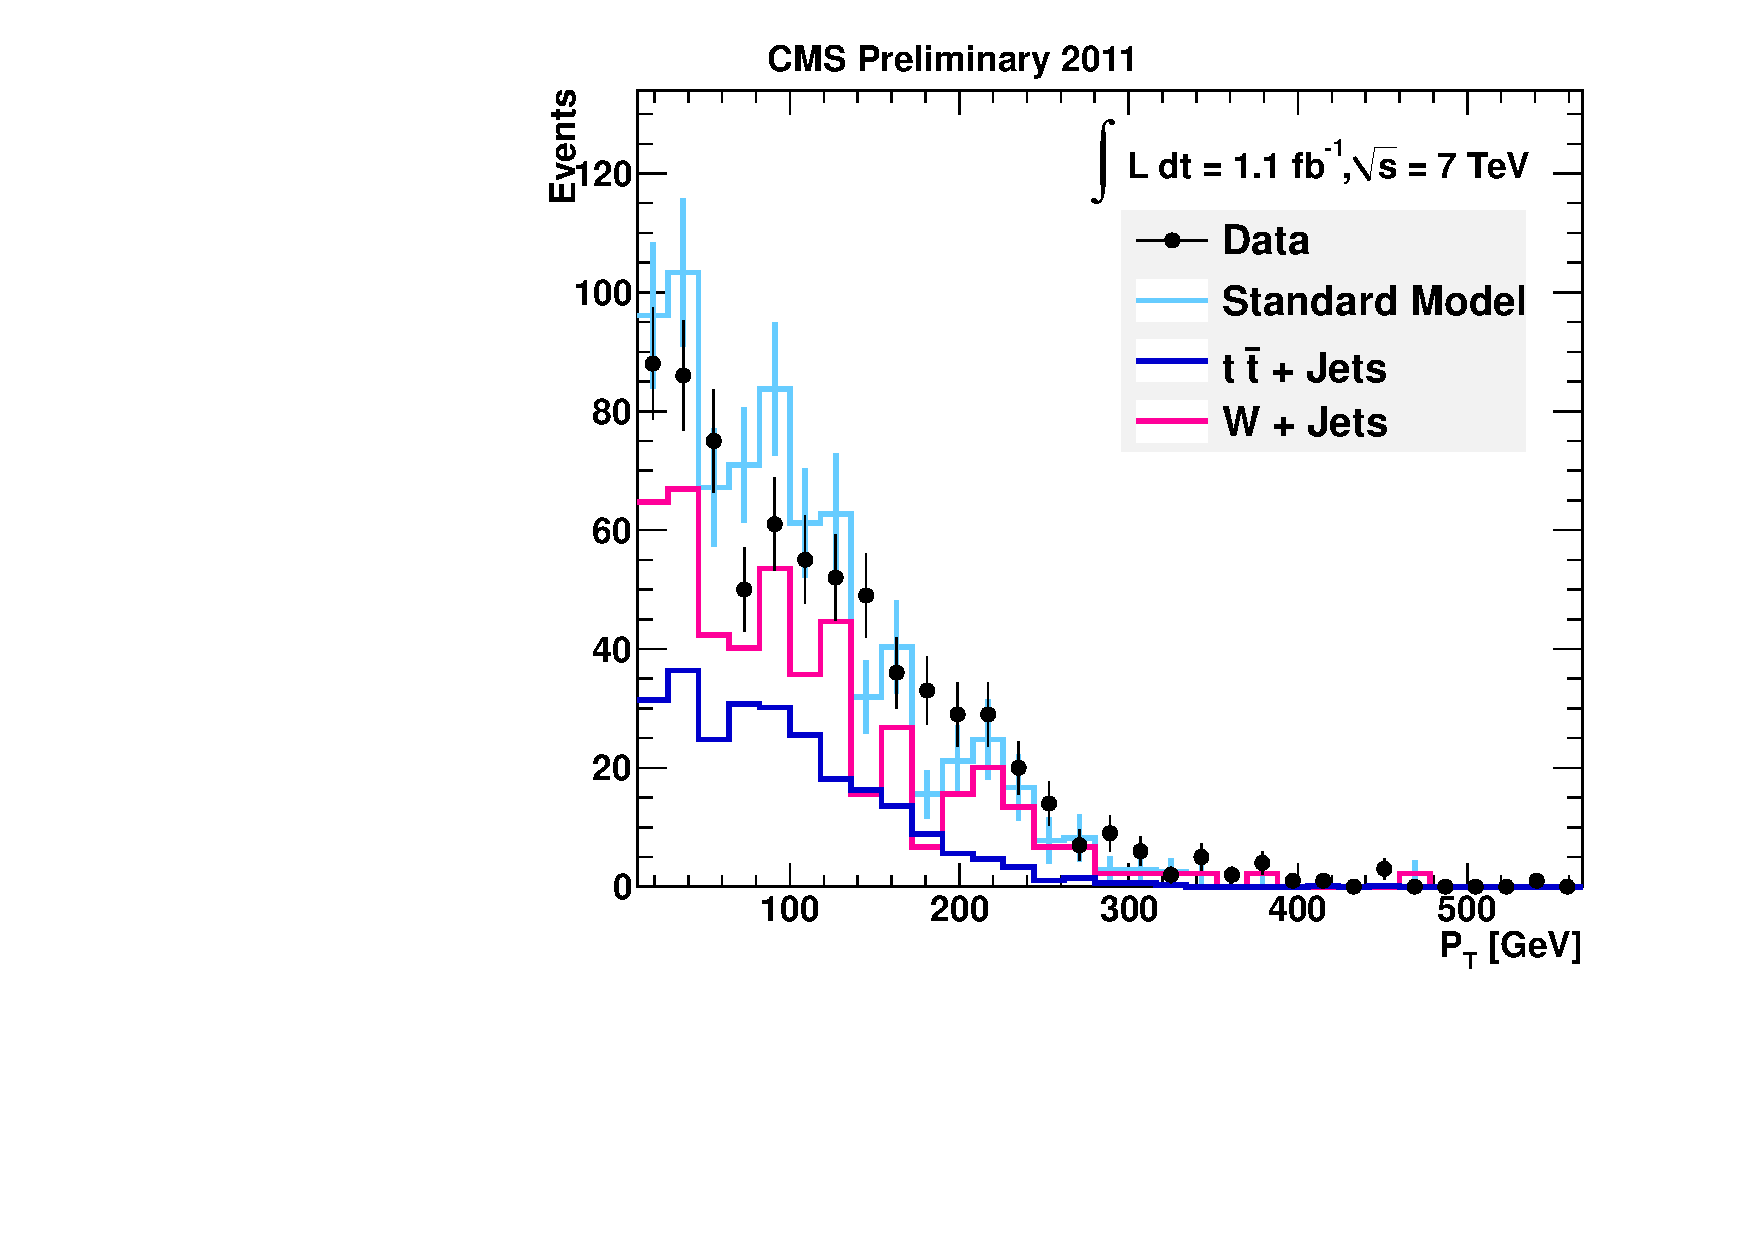
\includegraphics[width=0.45\textwidth, angle=0]{Figures/Analysis/PAS/muon_plots/spring11NoLogYMuPtMuonControl_afteraT.pdf}}
\subfigure[\label{fig:muon_beforeat_njet}]{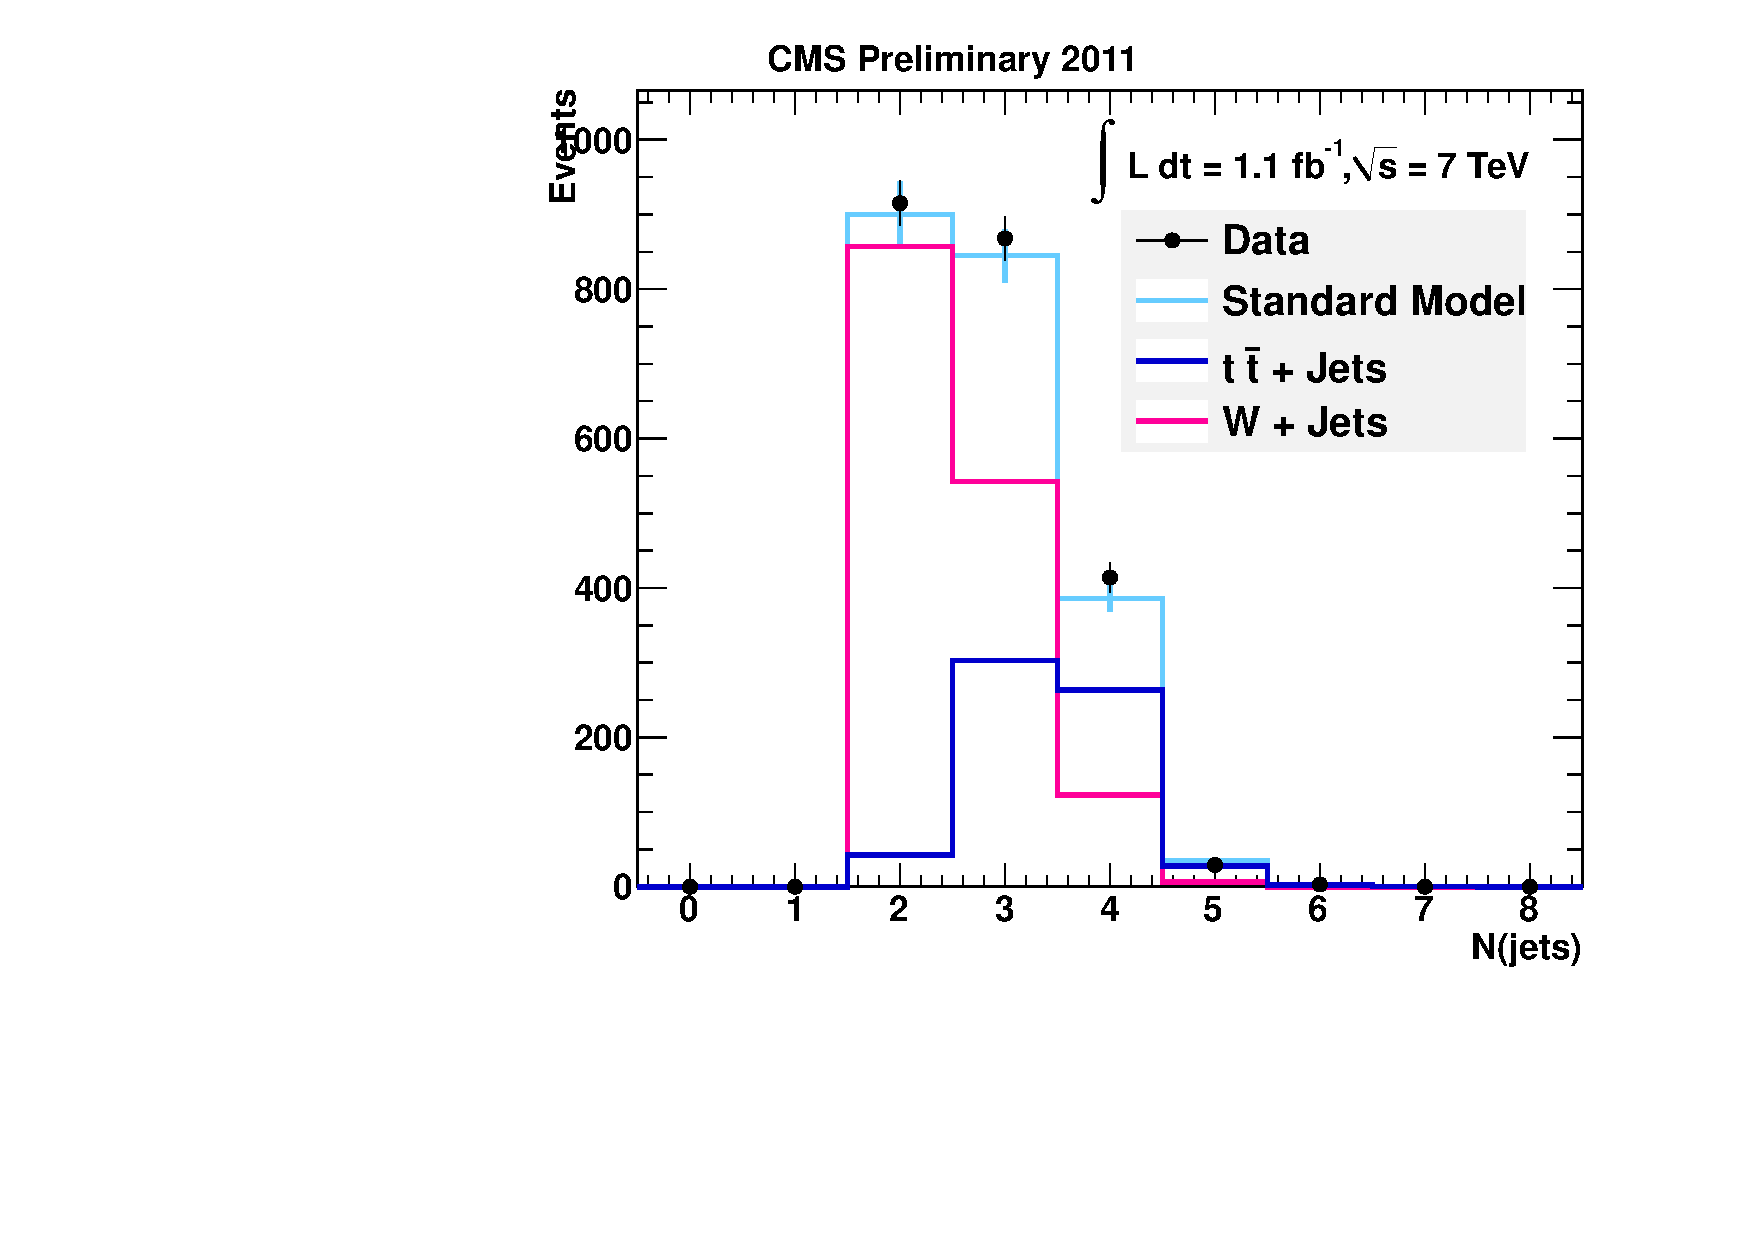
\includegraphics[width=0.45\textwidth, angle=0]{Figures/Analysis/PAS/muon_plots/spring11NoLogYnJetMuonControl_beforeaT.pdf}}
\newline

\subfigure[\label{fig:muon_afterat_at}]{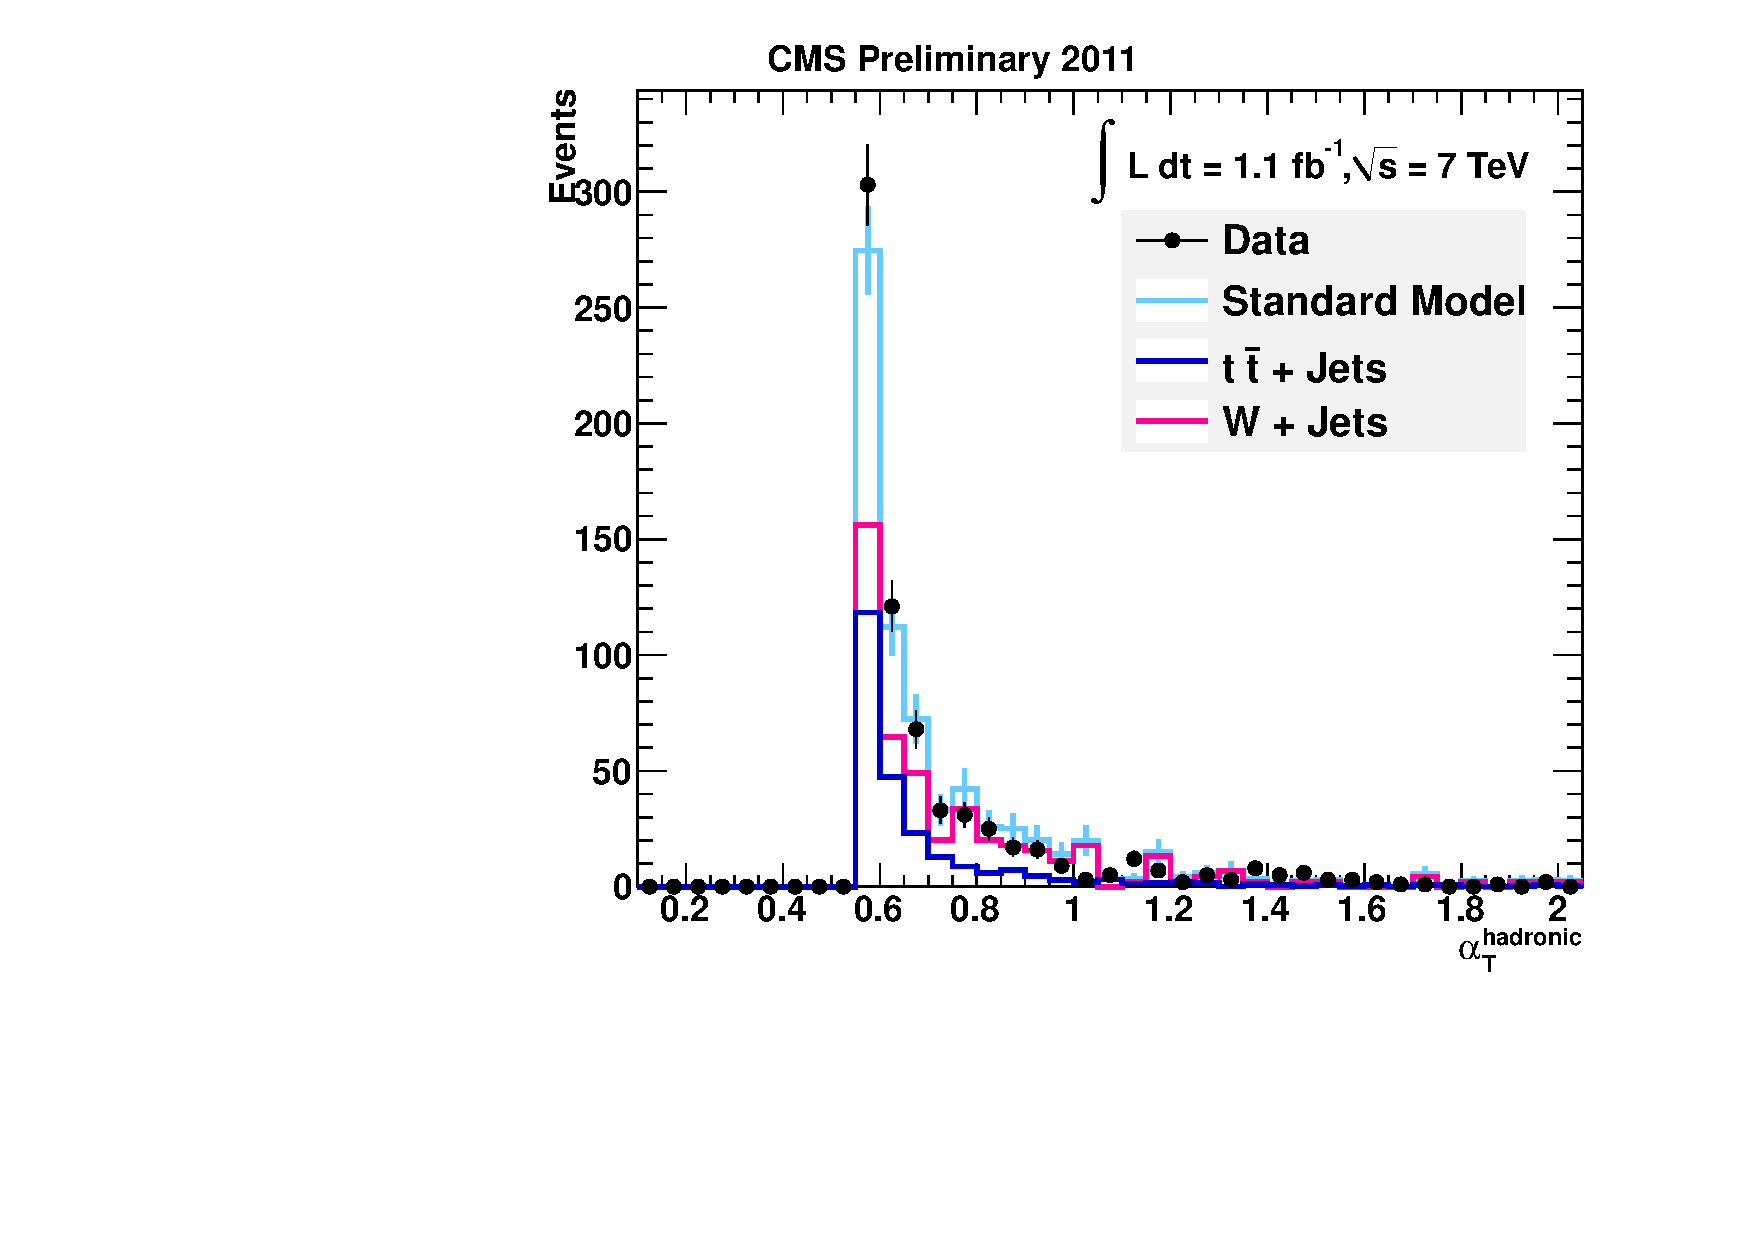
\includegraphics[width=0.45\textwidth, angle=0]{Figures/Analysis/PAS/muon_plots/spring11NoLogYaT_HMuonControl_afteraT.pdf}}
\subfigure[\label{fig:muon_afterat_ht}]{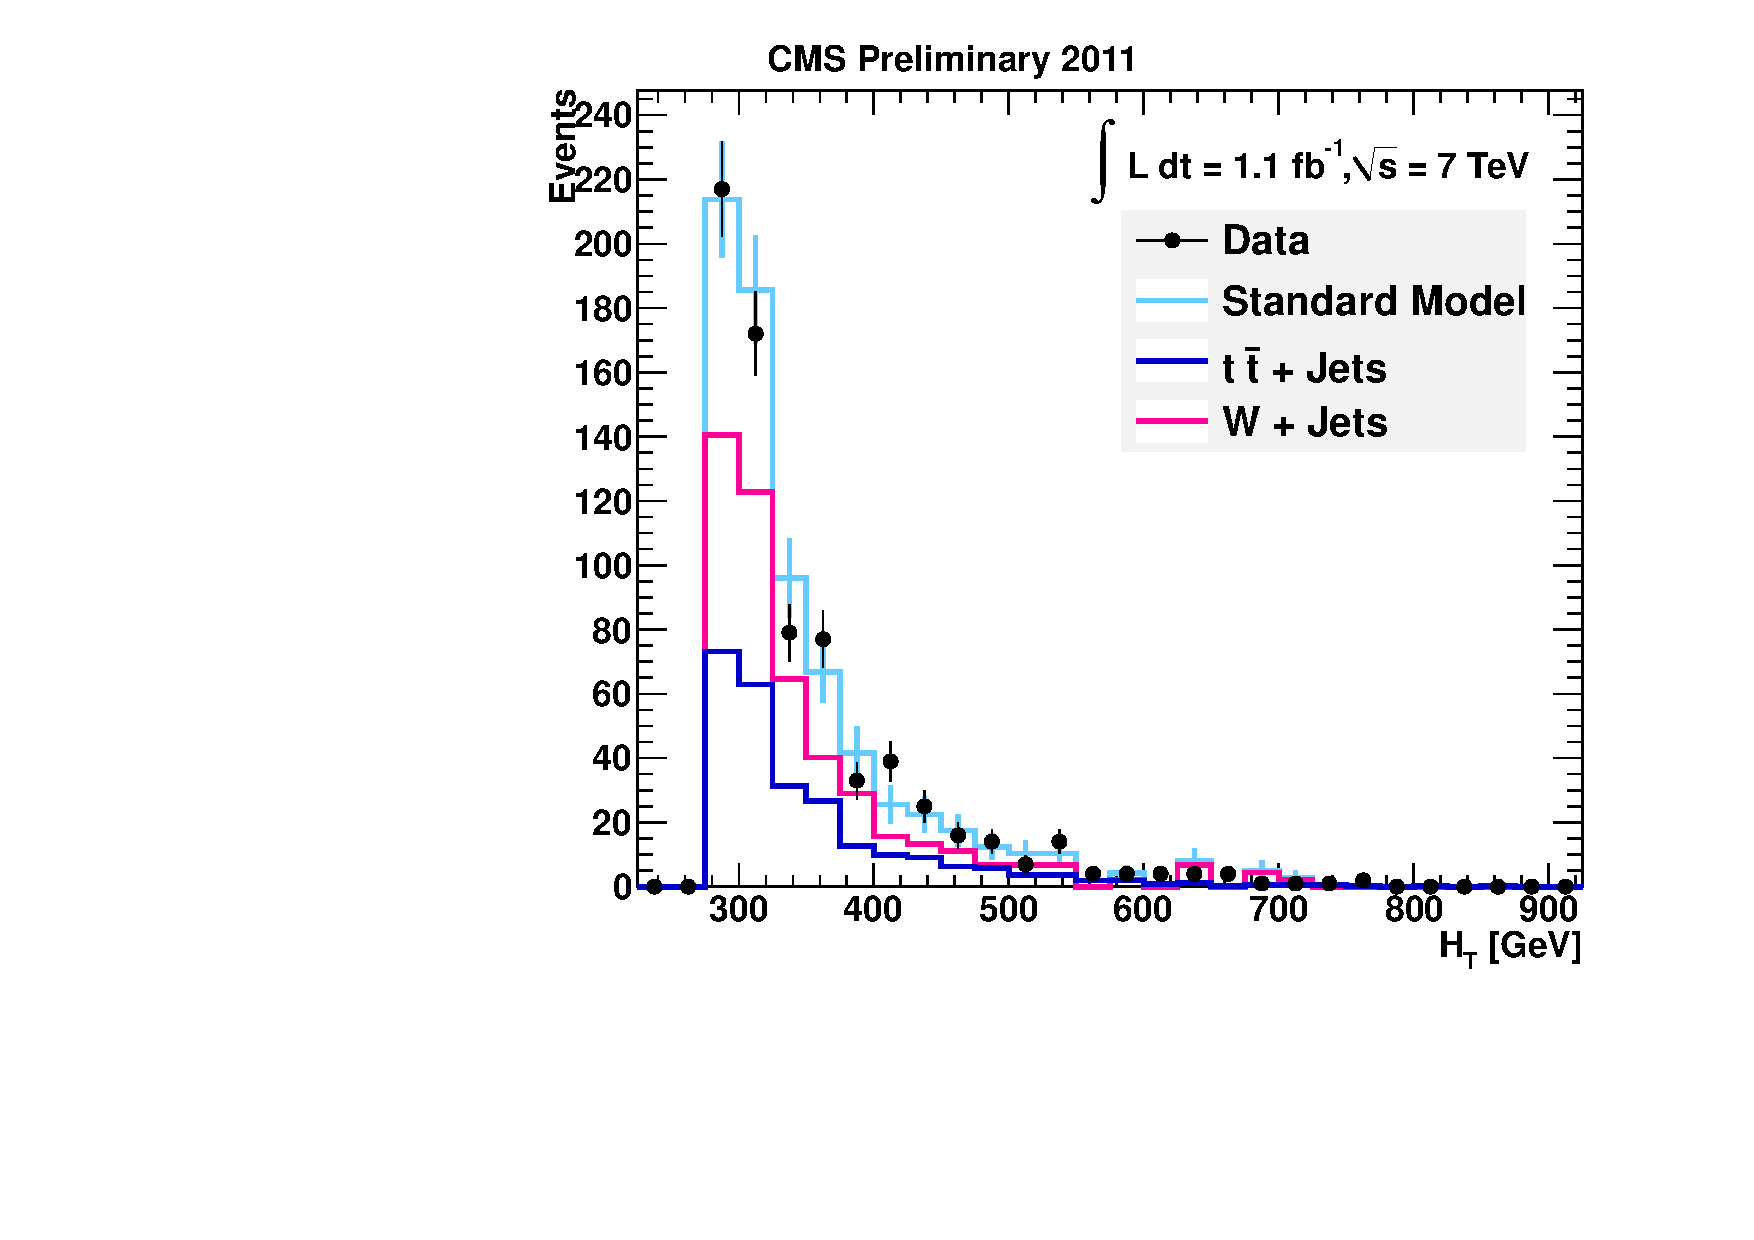
\includegraphics[width=0.45\textwidth, angle=0]{Figures/Analysis/PAS/muon_plots/spring11NoLogYHTMuonControl_afteraT.pdf}}
\newline
\subfigure[\label{fig:muon_afterat_MuIso}]{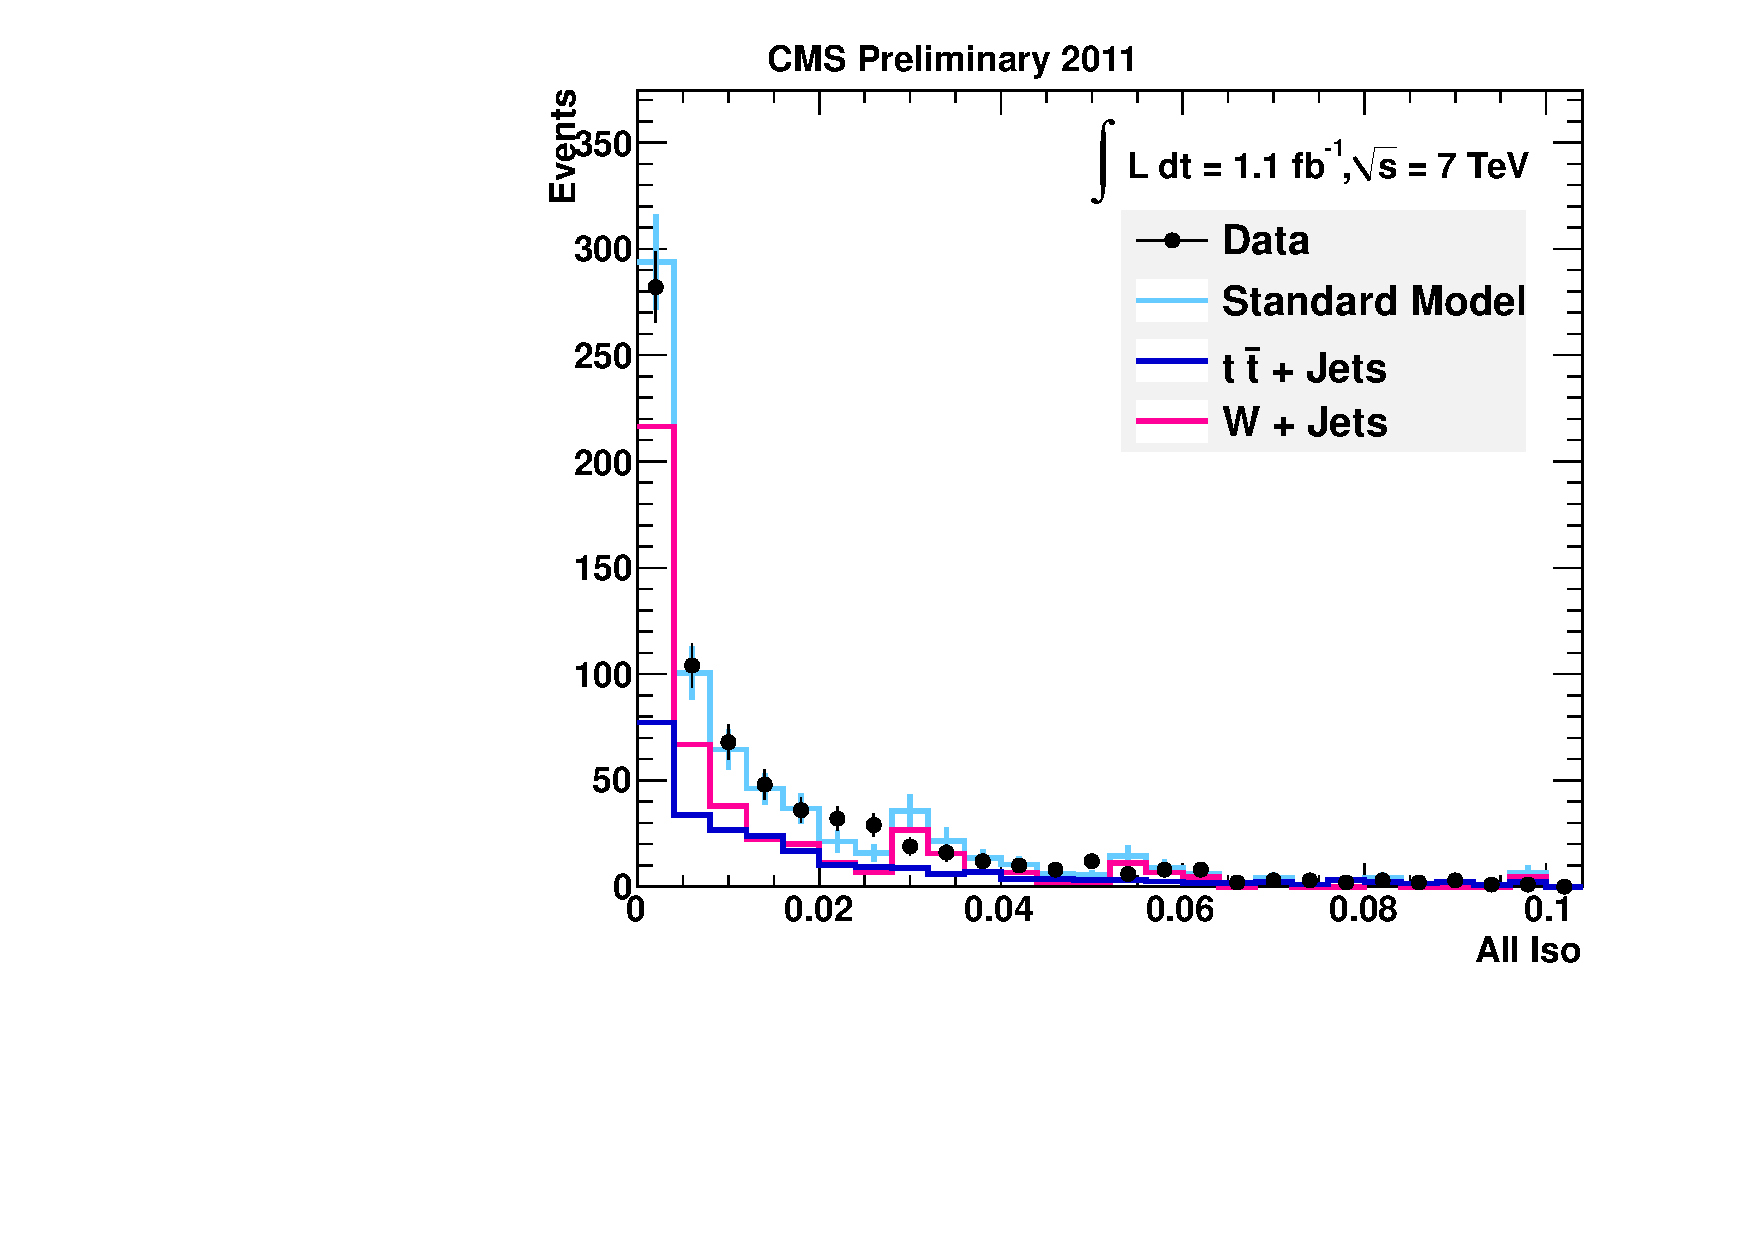
\includegraphics[width=0.45\textwidth, angle=0]{Figures/Analysis/PAS/muon_plots/spring11NoLogYMuCsoMuonControl_afteraT.pdf}}
\subfigure[\label{fig:muon_afterat_mt}]{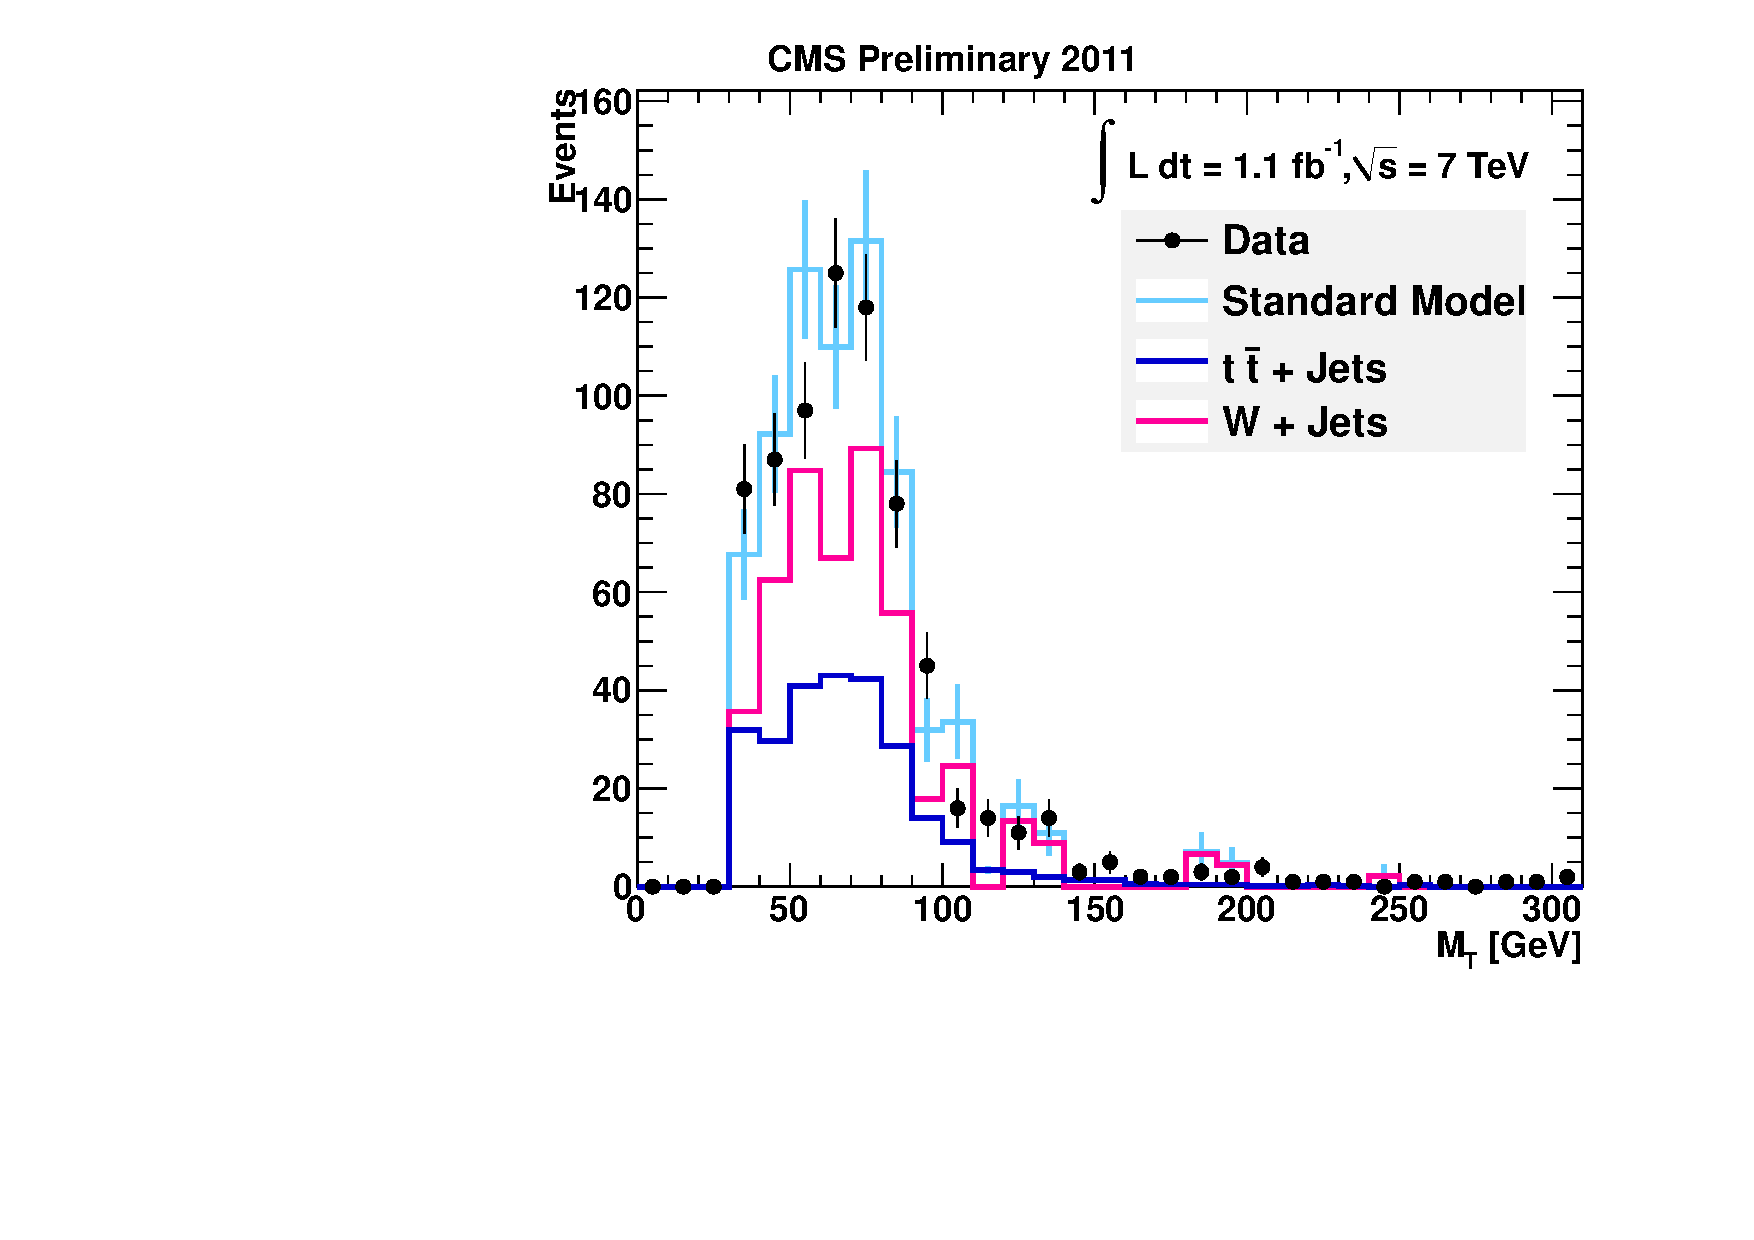
\includegraphics[width=0.45\textwidth, angle=0]{Figures/Analysis/PAS/muon_plots/spring11NoLogYMTMuonControl_afteraT.pdf}}

\caption{\label{fig:muonplots_afterat} Data - Monte Carlo comparisons
  for the muon control selection after the $\alpha_{T} > 0.55$ cut is
  applied, shown for (a) \scalht and (b) $M_T$, (c) Muon  Combined Isolation and (d) $M_{T}$.
 A cut of $\mathrm{HT >}$375 GeV has been applied, to select the
 region of fixed jet thresholds.}
\label{fig:kin}
\end{center}
\end{figure}

\subsubsection{Types of decay contributing to Muon Control Sample}

\begin{figure}[h]
\begin{center}
\subfigure[\label{fig:muon_types_275TT}]{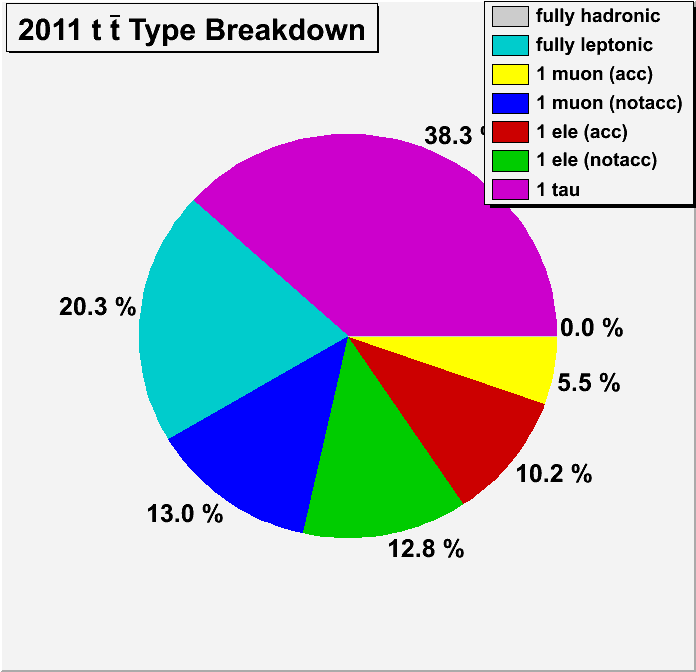
\includegraphics[width=0.40\textwidth, angle=0]{Figures/Analysis/Types/2011_275_TT_Pie}}
\subfigure[\label{fig:muon_types_275W}] {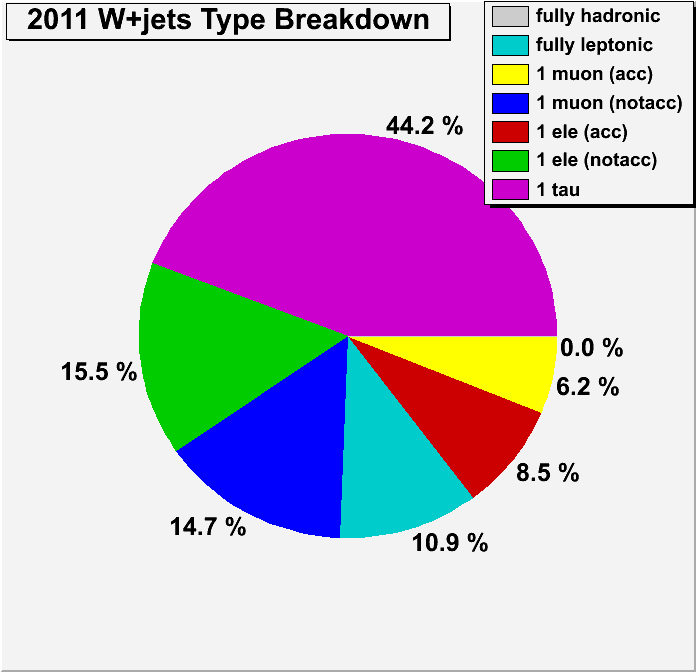
\includegraphics[width=0.40\textwidth, angle=0]{Figures/Analysis/Types/2011_275_W_Pie}}
\newline
\subfigure[\label{fig:muon_types_325TT}]{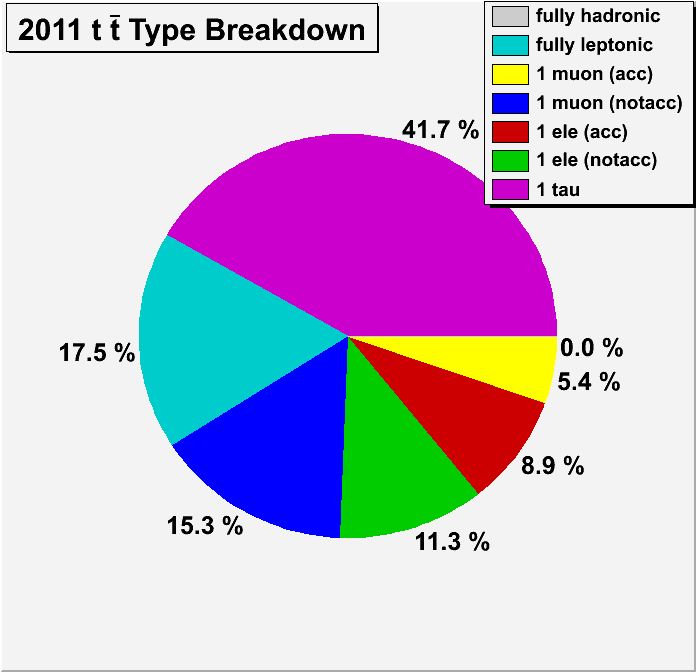
\includegraphics[width=0.40\textwidth, angle=0]{Figures/Analysis/Types/2011_325_TT_Pie}}
\subfigure[\label{fig:muon_types_325W}] {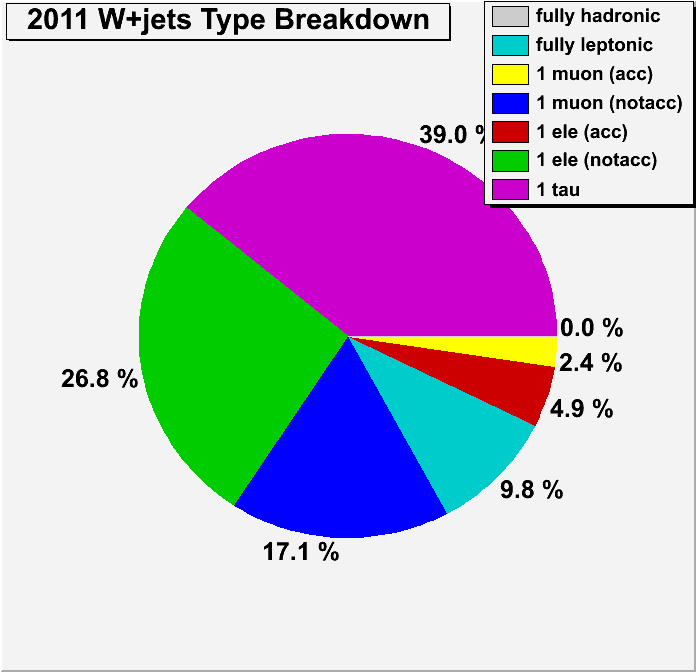
\includegraphics[width=0.40\textwidth, angle=0]{Figures/Analysis/Types/2011_325_W_Pie}}
\newline
\subfigure[\label{fig:muon_types_allTT}]{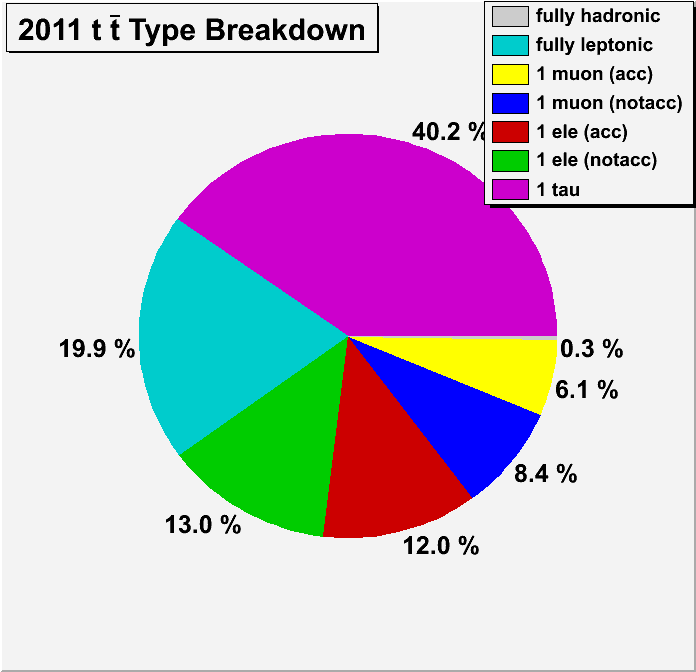
\includegraphics[width=0.40\textwidth, angle=0]{Figures/Analysis/Types/2011_unsca375_TT_Pie}}
\subfigure[\label{fig:muon_types_allW}] {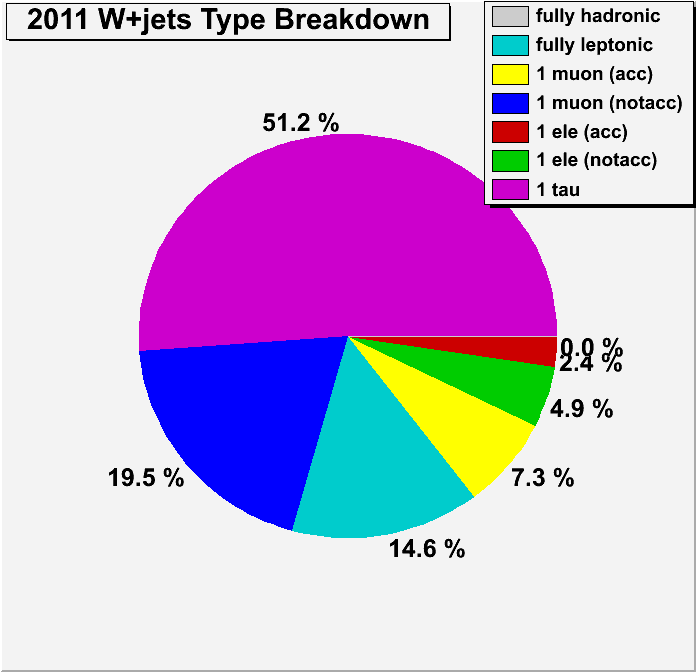
\includegraphics[width=0.40\textwidth, angle=0]{Figures/Analysis/Types/2011_unsca375_W_Pie}}

\caption{\label{fig:muon_types} Type breakdown of decays resulting in an event selected by the Muon Control selection, shown using Monte-Carlo truth information separately for \ttj (left) and \wj (right) events. The breakdown is made separately for each jet-scale case: 275 \less \HT \less 325 GeV (top), 325 \less \HT \less 375 GeV (middle), and \HT \more 375 GeV (bottom). }
\end{center}
\end{figure}

\subsection{Estimation Z  $\nu \bar{\nu}$ + jets background using photon + jets events}

\begin{figure}[h]
\begin{center}
\subfigure[\label{fig:photon_alphaT}]{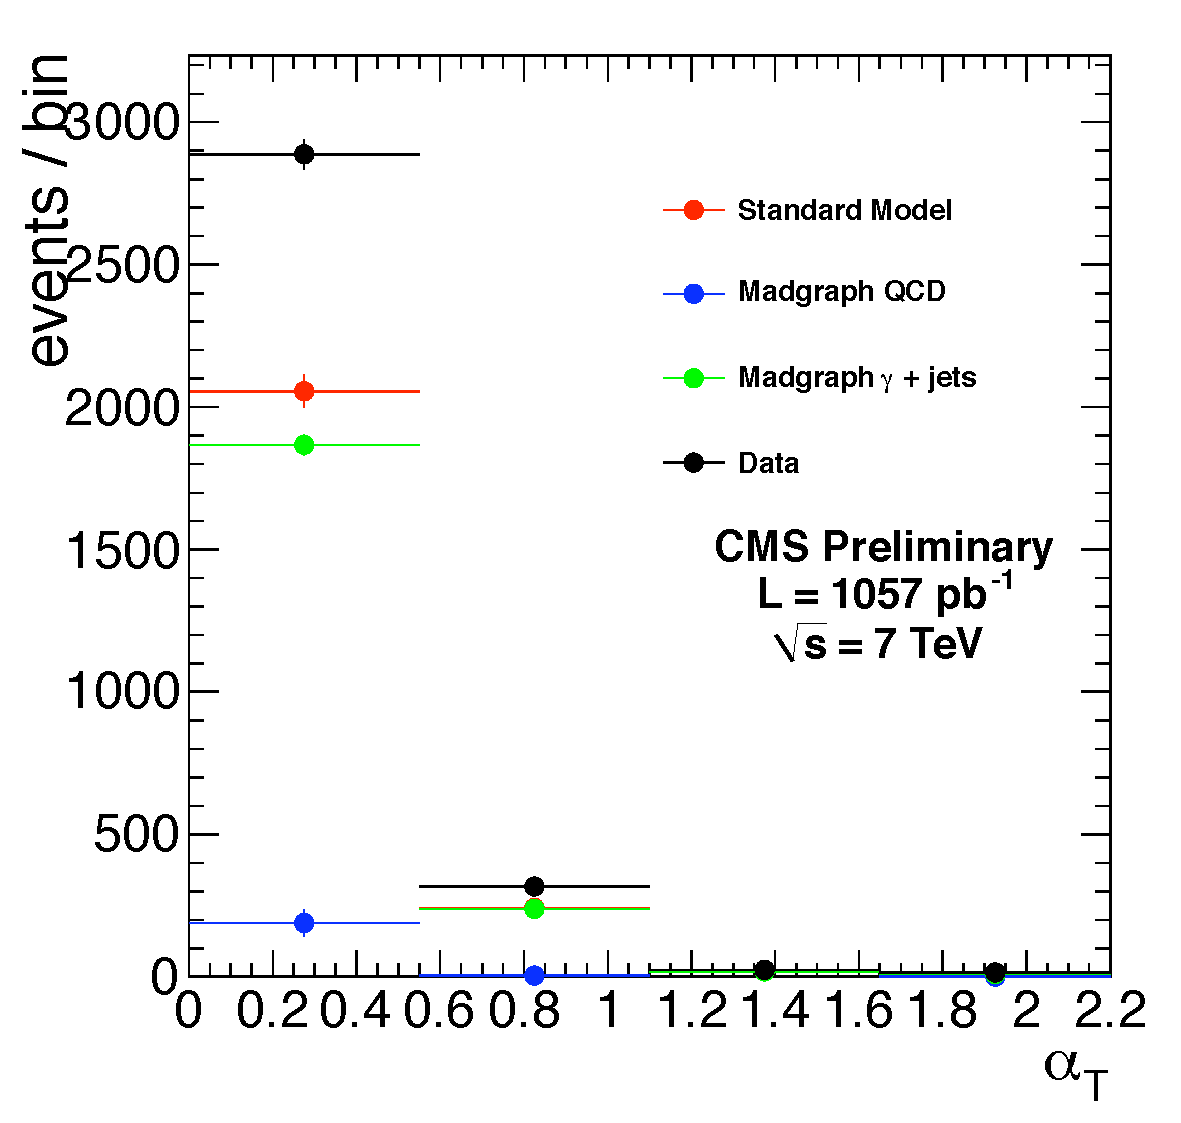
\includegraphics[width=0.45\textwidth, angle=0]{Figures/Analysis/PAS/photon_plots/375___xcak5JetAlphaTFewBinsPat.pdf}}
\subfigure[\label{fig:photon_nJets}] {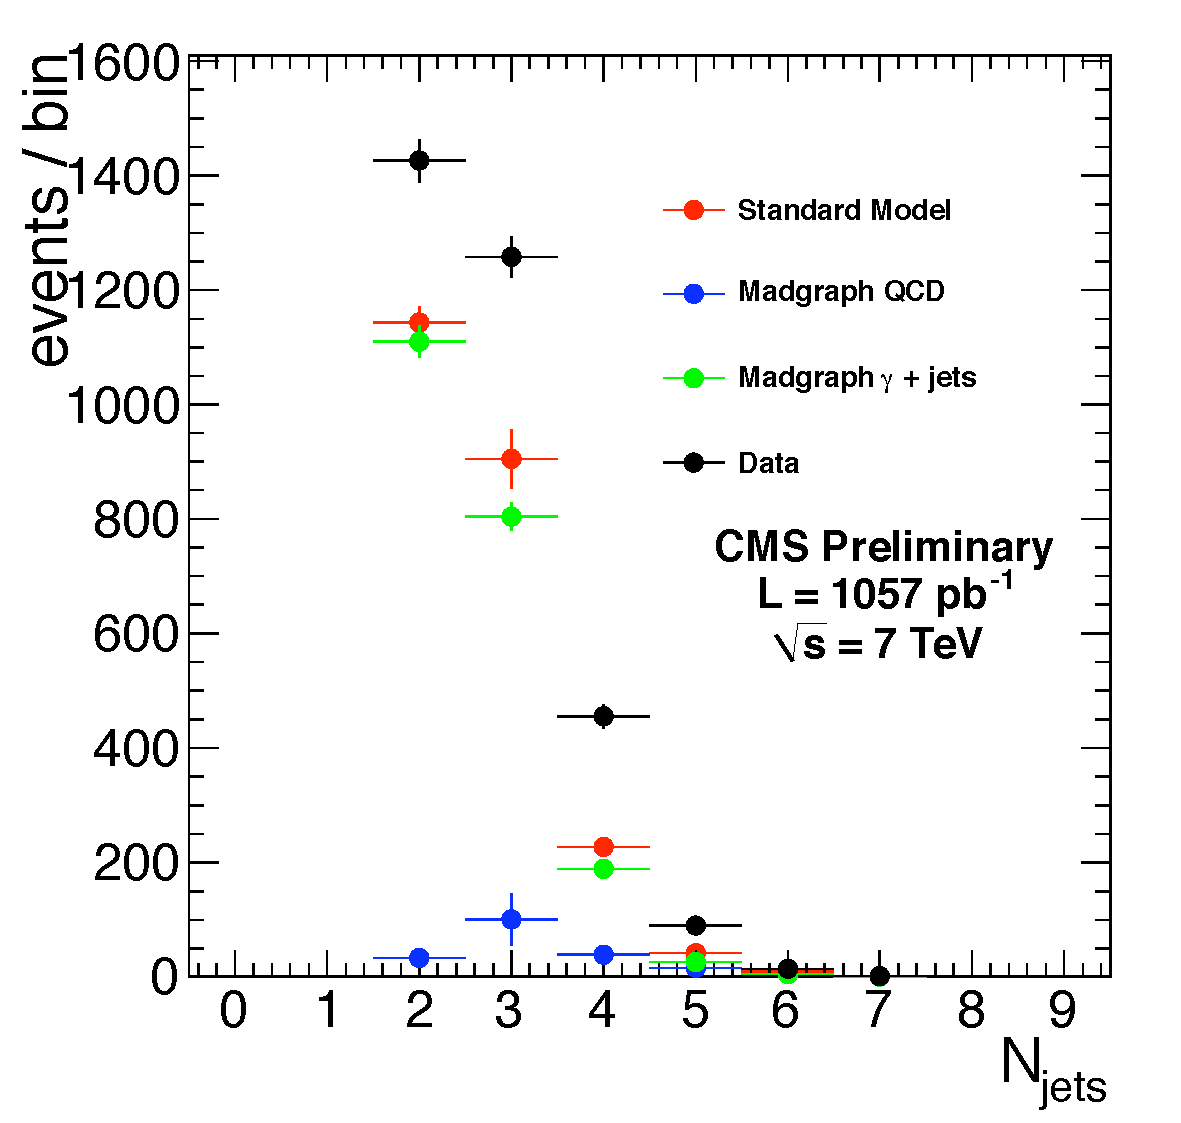
\includegraphics[width=0.45\textwidth, angle=0]{Figures/Analysis/PAS/photon_plots/375___xcak5JetIndicesPat.pdf}}
\caption{\label{fig:photon_plots} Data-MC comparisons for the photon control sample.  $\scalht > 375$~GeV and $\mht/\scalht>0.4$ are required.   Left: the distribution of $\alpha_{T}$.  Right: the distribution of the number of jets.}
\end{center}
\end{figure}

\section{Systematic Uncertainties}
\section{Simultaneous Fit}


 \begin{figure}[h]
   \begin{center}
     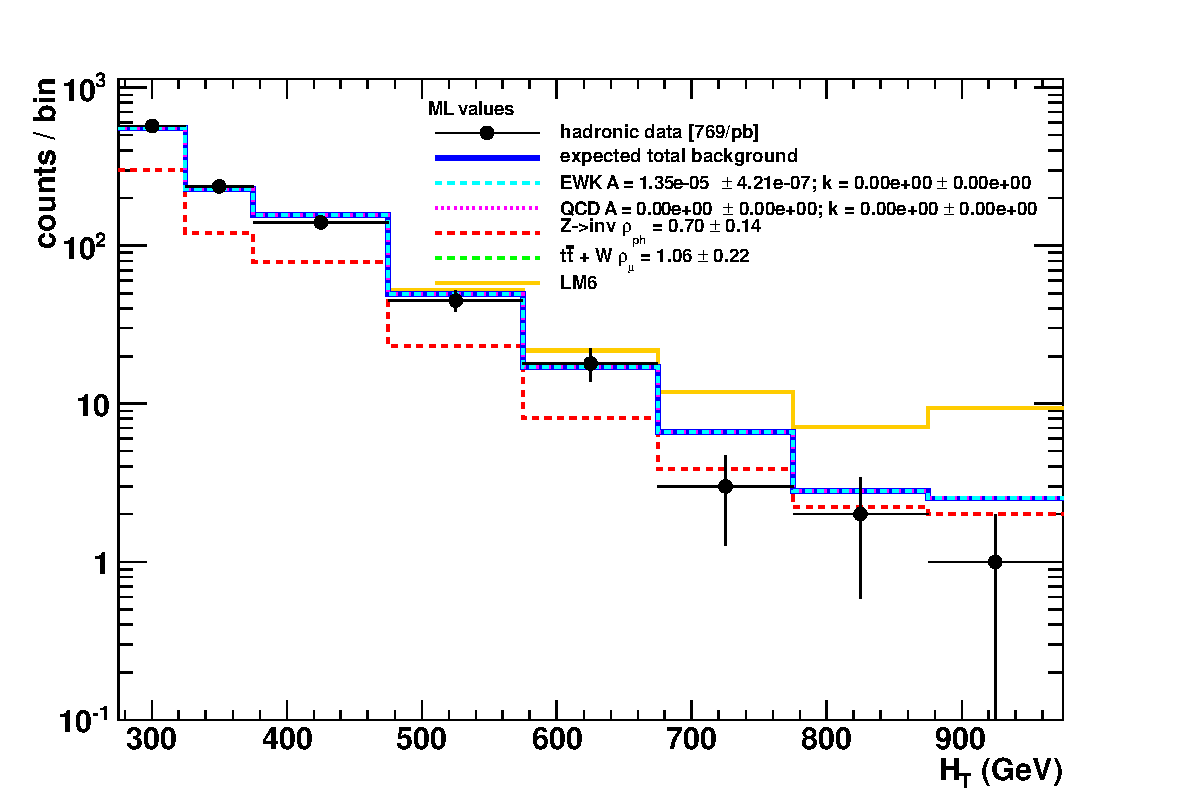
\includegraphics[width = 0.48\textwidth]{Figures/Analysis/PAS/stats_plots/RQcdZero/hadronic_signal_fit_logy.pdf}
     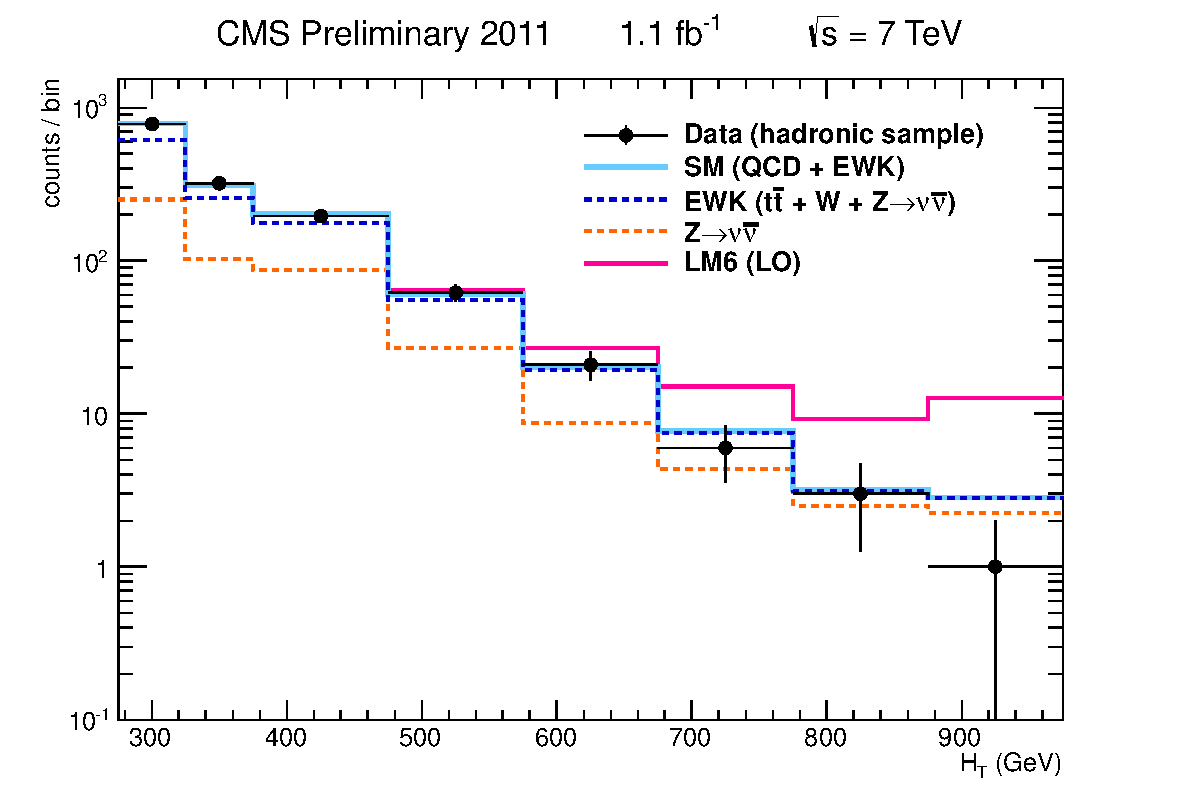
\includegraphics[width = 0.48\textwidth]{Figures/Analysis/PAS/stats_plots/RQcdFallingExp/hadronic_signal_fit_logy.pdf}
     \caption{\label{fig:hadronic} \scalht distribution for events in the hadronic signal sample for scenario a) (left) and scenario b) (right). Shown are the events observed in data (black points), the outcome of the fit (blue line) and a breakdown of the individual background contributions as predicted by the control samples. A possible signal contribution from benchmark point LM6 is indicated as well (yellow line).}
   \end{center}
 \end{figure}

 \begin{figure}[h]
   \begin{center}
     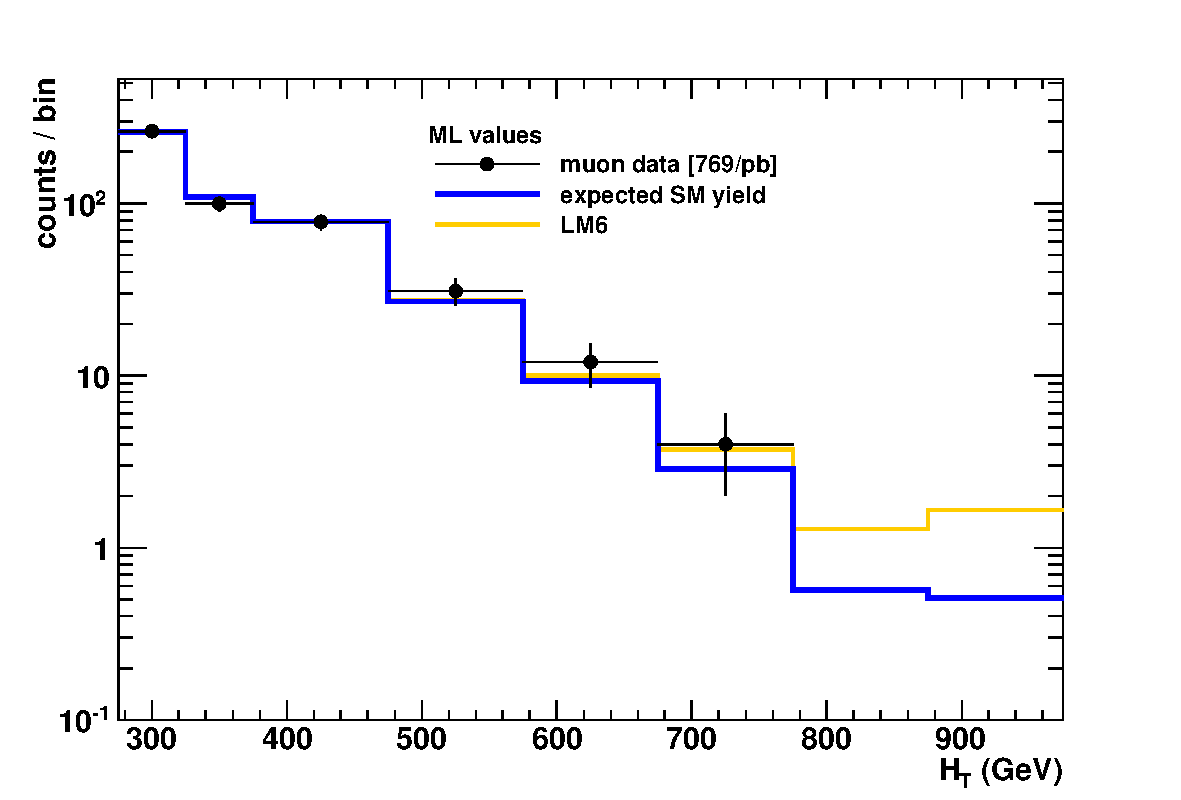
\includegraphics[width = 0.48\textwidth]{Figures/Analysis/PAS/stats_plots/RQcdZero/muon_control_fit_logy.pdf}
     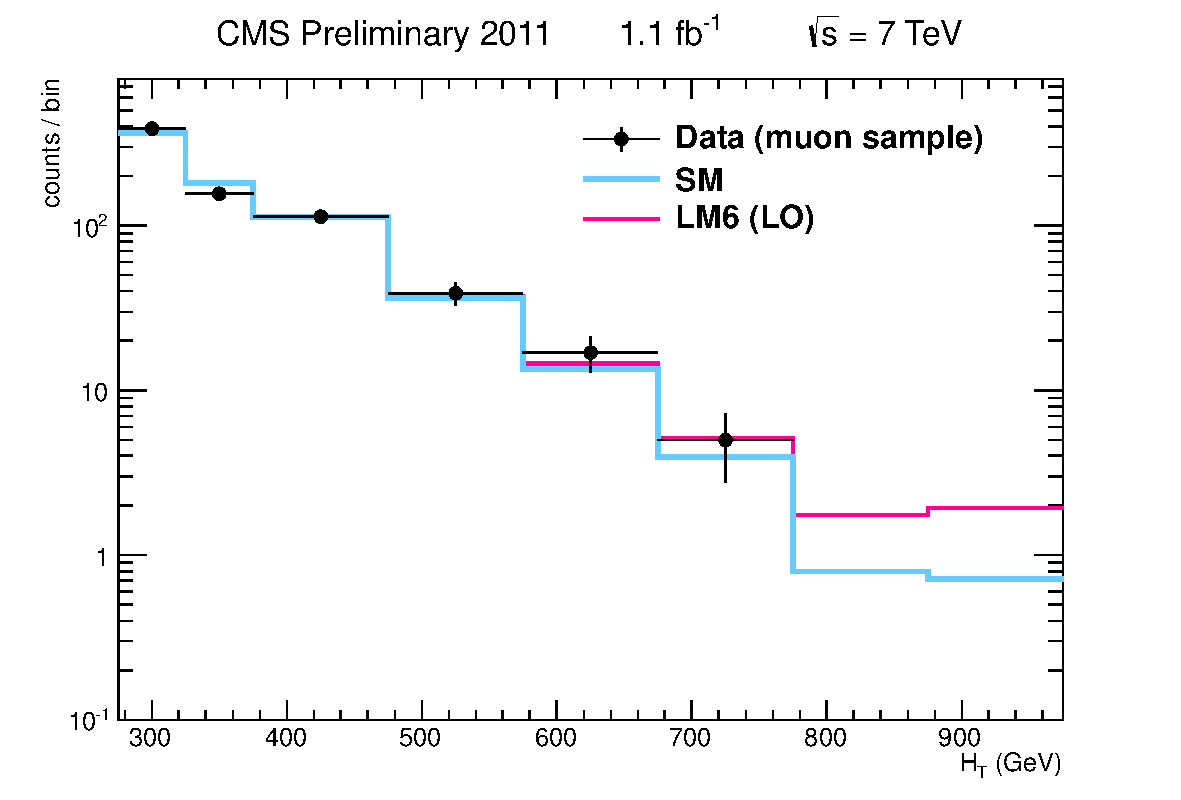
\includegraphics[width = 0.48\textwidth]{Figures/Analysis/PAS/stats_plots/RQcdFallingExp/muon_control_fit_logy.pdf}
     \caption{\label{fig:muon}  \scalht distribution for events selected in the muon control sample for scenario a) (left) and scenario b) (right).
  Shown are the events observed in data (black points), the outcome of the fit (blue line) and the MC expectation (dashed line). A possible signal
 contribution from benchmark point LM6 is indicated as well (yellow line).}
   \end{center}
 \end{figure}

 \begin{figure}[h]
   \begin{center}
     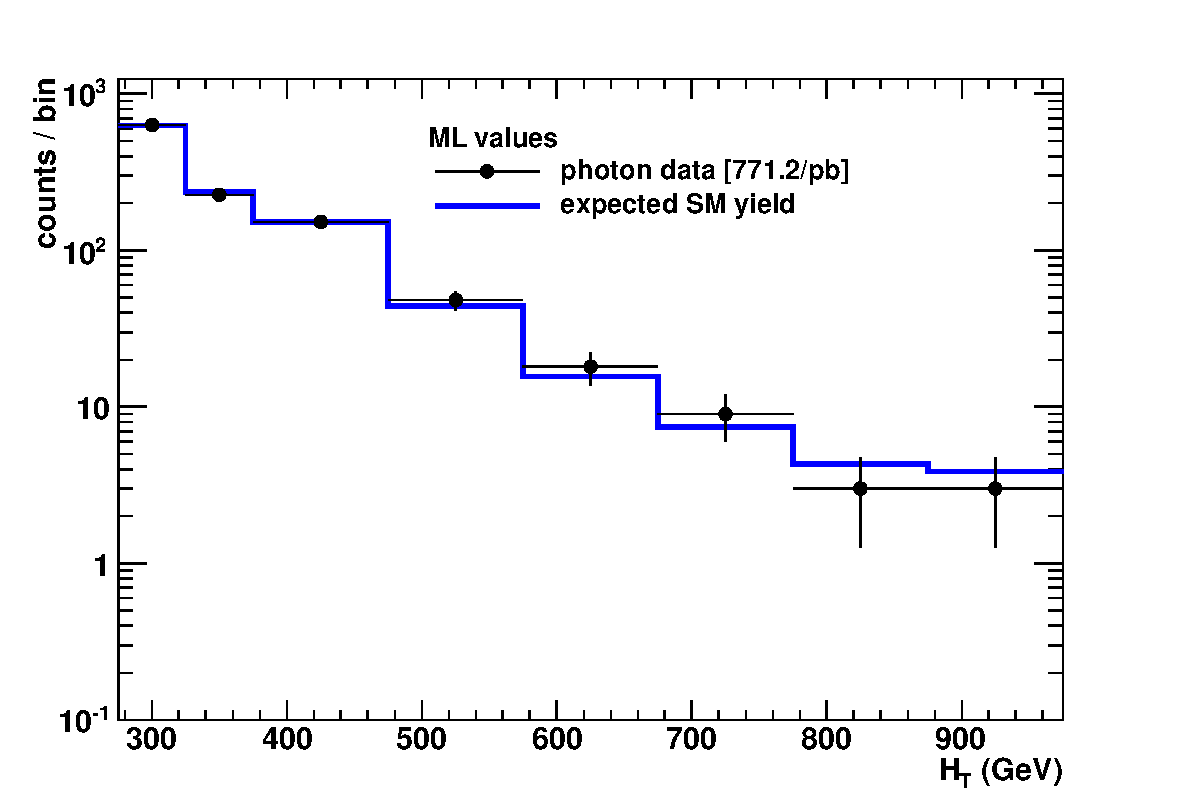
\includegraphics[width = 0.48\textwidth]{Figures/Analysis/PAS/stats_plots/RQcdZero/photon_control_fit_logy.pdf}
     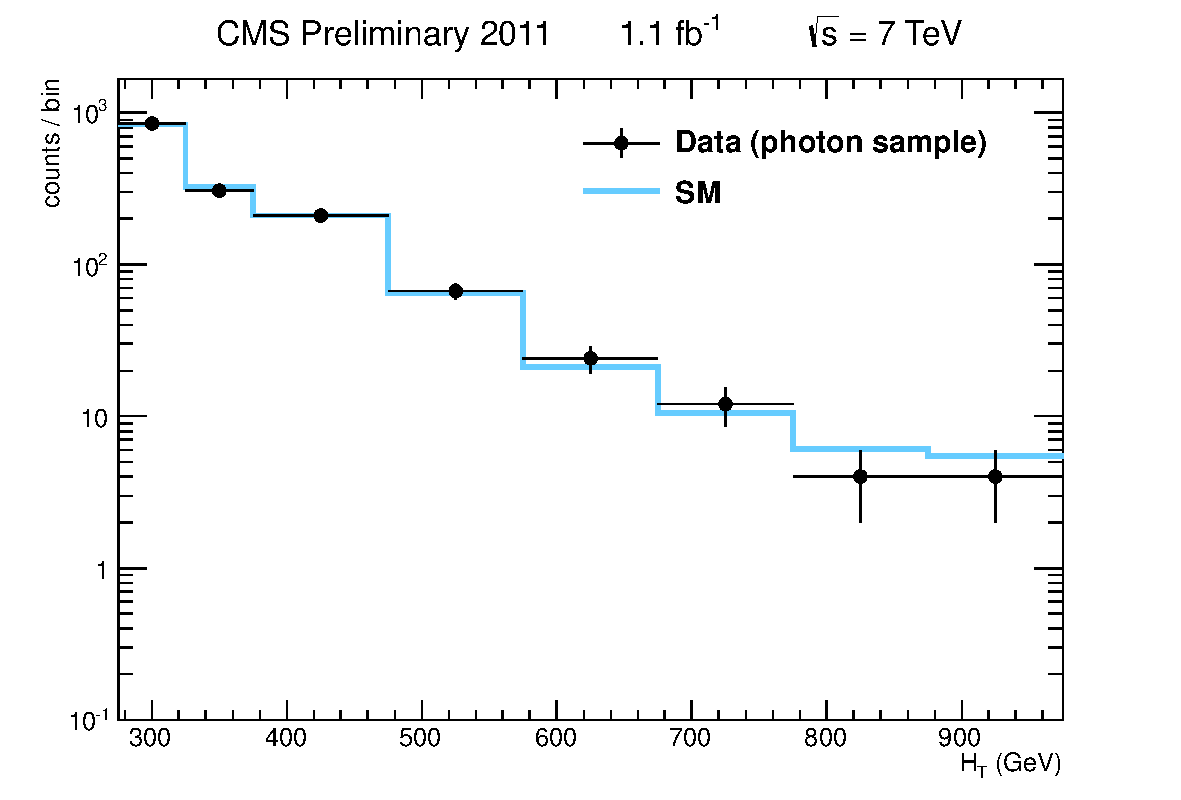
\includegraphics[width = 0.48\textwidth]{Figures/Analysis/PAS/stats_plots/RQcdFallingExp/photon_control_fit_logy.pdf}
     \caption{\label{fig:photon} \scalht distribution for events selected in the photon control sample for scenario a) (left) and scenario b) (right). Shown are the events observed in data (black points), the outcome of the fit (blue line) and the MC expectation (dashed line).}
   \end{center}
 \end{figure}

 \begin{figure}[h]
   \begin{center}
     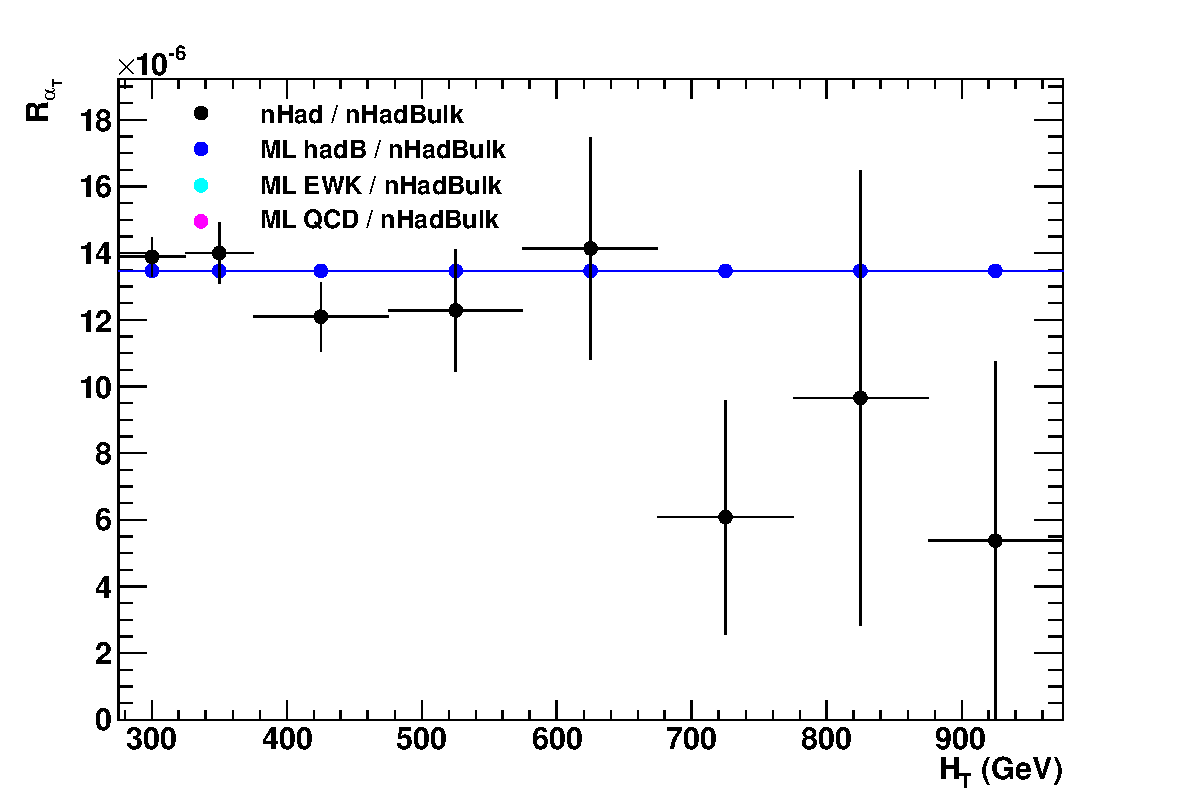
\includegraphics[width = 0.48\textwidth]{Figures/Analysis/PAS/stats_plots/RQcdZero/hadronic_signal_alphaT_ratio.pdf}
     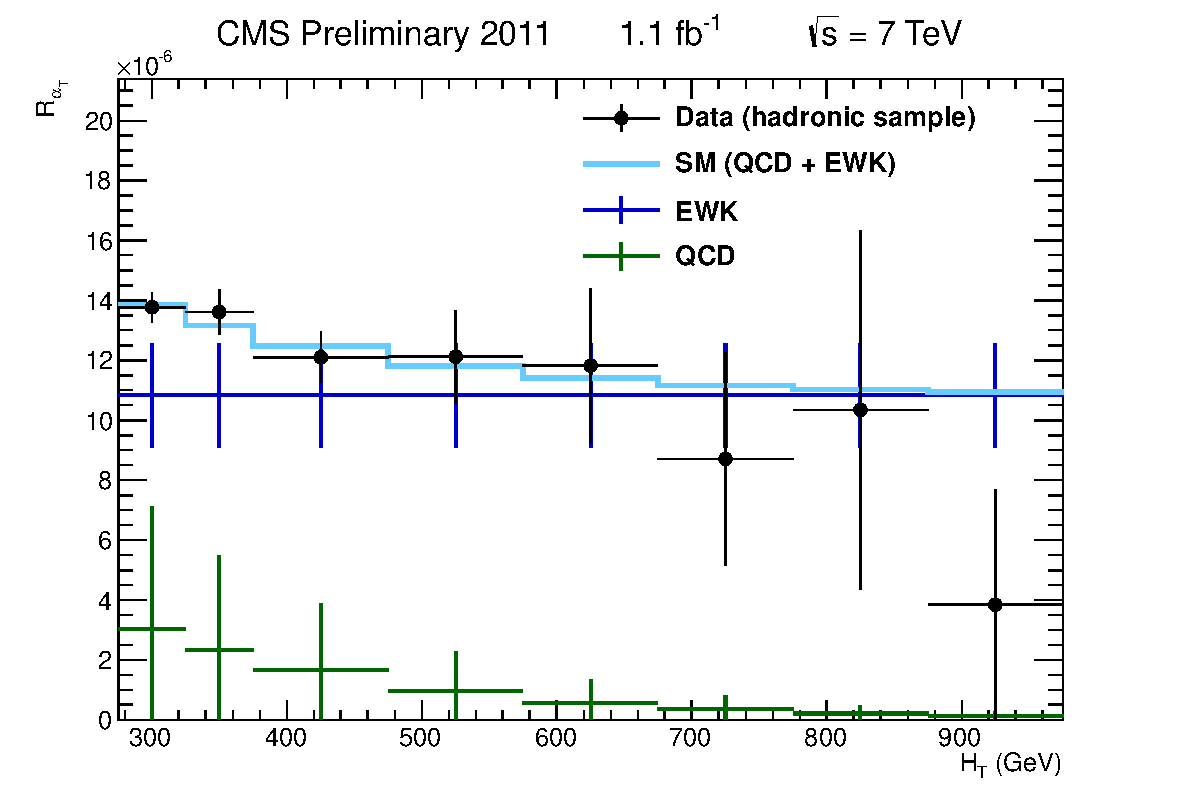
\includegraphics[width = 0.48\textwidth]{Figures/Analysis/PAS/stats_plots/RQcdFallingExp/hadronic_signal_alphaT_ratio.pdf}
     \caption{\label{fig:rat} \RaT as a function of \scalht as observed in data (black points) and the results of the fit assuming different scenarios: a) (left) and b) (right) .}
   \end{center}
 \end{figure}

\section{Limits}

\begin{figure}[h]
  \begin{center}
    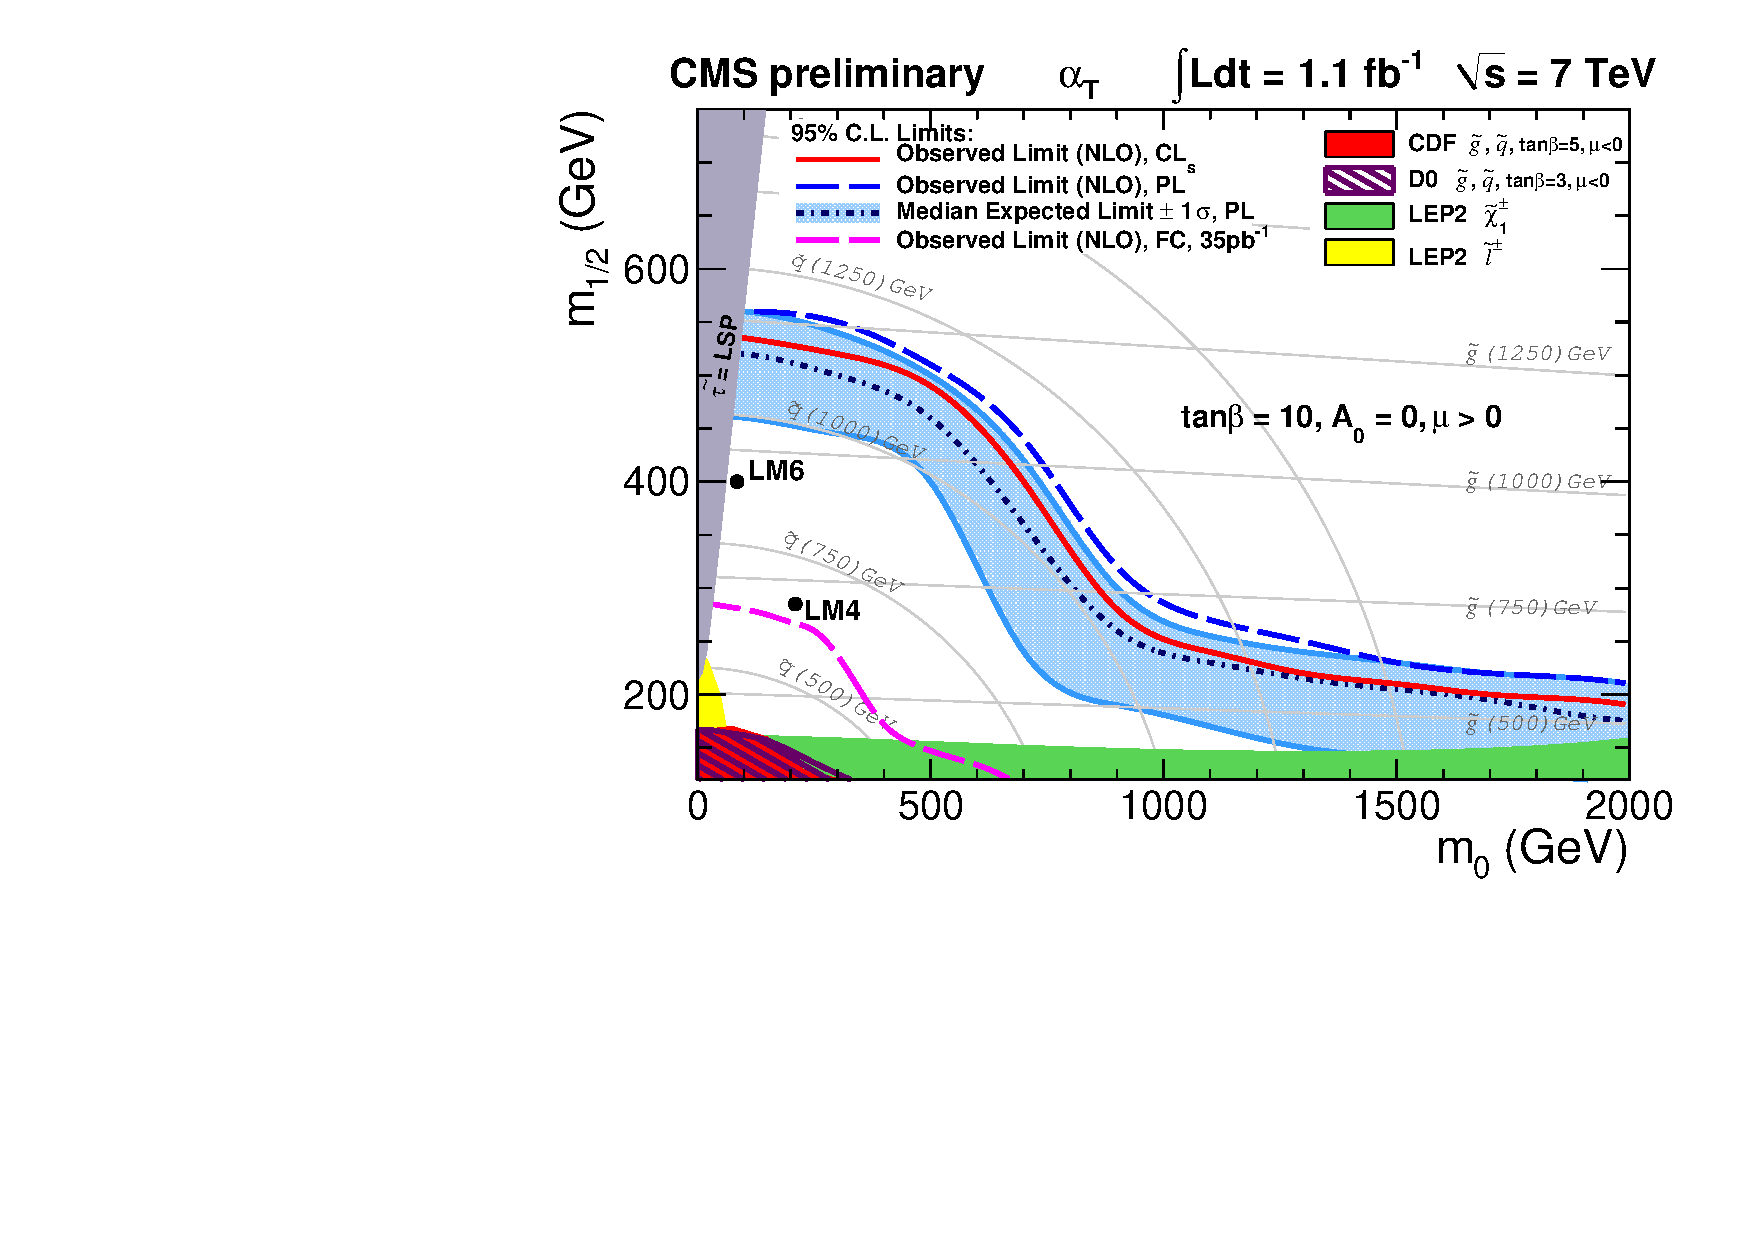
\includegraphics[width = 0.90\textwidth]{Figures/Analysis/PAS/RA1_ExclusionLimit_tanb10_def.pdf}
    \caption{\label{fig:cmssm} Observed and expected 95\% CL exclusion
      contours in the CMSSM ($m_0, m_{1/2}$) plane ($\tan \beta = 10,
      A_0 = 0, \mu > 0$) using NLO signal cross sections using the
      Profile Likelihood (PL) method. The expected limit is shown with
      its 68\% CL range.  The observed limit using the $\cls$ method is
      shown as well.  }
  \end{center}
\end{figure}


\section{Conclusion}


%\chapter{Extending the $\mu$ Control Sample to a Signal Sample}
\ref{ch:ra4}

In Chapter~\ref{ch:RA1}, the $\mu$ control sample was used effectively to predict the background contribution from W and \tto events. The $\mu$ likelihood's incorporation into the overall likelihood in order to interpret the hadronic results allowed for some small signal contamination. However it was in general viewed as a constraint on the ``signal" region of the hadronic selection. 

The cuts outlined in Section~\ref{sec:musel} are designed to select events from Standard Model W decays, hence minimising the contamination from signal. However, as the simultaneous fit includes the signal efficiency in the $\mu$ control sample it is possible to relax the cuts and allow more potential signal into the $\mu$ yield. The following work represents the author's personal investigation into the effect of increasing the chance for signal contamination on the eventual limit. 

\subsection{Relaxing the Cuts}

The primary cut in the $\mu$ control sample responsible for restricting the signal is the M$_{T}$ requirement, as it puts a restriction on boosted W decays. The first step is to remove this cut, allowing more potential signal into the sample. Having done so there are three possible scenarios with respect to the \alt cut:

\begin{itemize}
\item Use the \alt cut from the hadronic analysis, where the muon is ignored
\item Take out the \alt cut to increase statistics in the $\mu$ sample (the MHT/HT cut ensures the elimination of QCD background)
\item Adapt the definition of the \alt to include the lepton, the validity of which is shown in Section~\ref{sec:lalt}
\end{itemize}

Using the \alt cut as defined in the hadronic analysis is a natural choice. However the use of an \alt cut limits the statistics, so removing this cut would increase the $\mu$ sample statistics. Conversely, using the hadronic definition of the \alt cut without concerning the $\mu$ leads to the appearance of missing energy, hence allowing more background into the sample. The use of the $\alt^{lep}$ cut as defined in Section~\ref{sec:lalt} removes this issue, but decreases statistics. 

The one muon requirement cut and the other cuts mentioned in Section~\ref{sec:muon} remain as they do not pertain to the rejection of signal but rather the selection of a good isolated muon not overlapping with a jet, in the case where the decay is not from a Z where a second $\mu$ is not identified by the quality criteria. The \MHT / \HT cut is generally superseded by the \alt cut therefore removing it has little effect, however it is left in so that in the case where the \alt cut is removed we remain in the kinematic pause space of the hadronic signal region. 

 

\subsection{Event Yields}

\begin{table}[htbp]
\centering
\footnotesize
\begin{tabular*}{0.99\linewidth}{@{\extracolsep{\fill}}c c c c c c}
\hline
\hline
& \scalht Bin (GeV) & 275--325 & 325--375 & 375--475 & 475--575 \\ [0.5ex]
\hline
\hline
\multirow{3}{*}{2011 Selection} & B (SM) &407.5 & 179.1  & 131.6 & 48.7 \\
&S (LM6)&0.15 & 0.15 & 0.53 & 0.82\\
& S / B & 0.000 & 0.001 & 0.004 & 0.017\\
\hline
\multirow{3}{*}{a) No M$_{T}$ Cut \& \alt $>$ 0.55} & B (SM) &549.93 &243.33&179.51 &63.80 \\
&S (LM6)& 0.19 & 0.20 & 0.59 & 0.92 \\
& S/B & 0.000 & 0.001 & 0.003 & 0.0014 \\
\hline
\multirow{3}{*}{b) No M$_{T}$ Cut \& No \alt} & B (SM) &1335.81& 603.61 & 485.62 & 192.61\\
&S (LM6) &0.26&0.32&0.89&1.43\\
& S/B & 0.000 & 0.001 & 0.002 & 0.007 \\
\hline
\multirow{3}{*}{c) No M$_{T}$ Cut \& \alt$_{lep}$ $>$ 0.55} & B (SM) & 163.95 & 70.64 & 39.87  & 16.38  \\
& S (LM6) & 0.13 & 0.17 & 0.51 & 0.79 \\
& S/B & 0.001 & 0.002 & 0.013 & 0.048 \\
\hline
\hline
\end{tabular*}
\newline
\newline
\newline
\begin{tabular*}{0.99\linewidth}{@{\extracolsep{\fill}}c c c c c c}
\hline
\hline
& \scalht Bin (GeV) & 575--675 & 675--775 & 775--875 & 875--$\infty$  \\ [0.5ex]
\hline
\hline

\multirow{3}{*}{2011 Selection} & B (SM) &13.32  & 7.95  & 3.20 & 0.97 \\
&S (LM6)&1.09 & 1.17 & 0.95 & 1.21\\
& S / B & 0.082 & 0.147 & 0.297 & 1.343\\
\hline
\multirow{3}{*}{a) No M$_{T}$ Cut \& \alt $>$ 0.55} & B (SM) & 18.53 & 8.59 & 3.34 & 0.97 \\
&S (LM6)& 1.23 & 1.35 & 1.08 & 1.42 \\
& S/B & 0.066 & 0.157 & 0.324 & 1.5747 \\
\hline

\multirow{3}{*}{b) No M$_{T}$ Cut \& No \alt} & B (SM) & 67.64 & 30.04 & 12.77 & 3.26 \\
&S (LM6) &1.87 & 2.04 & 1.77 & 3.07\\
& S/B & 0.028 & 0.068 & 0.139 & 0.940 \\
\hline
\multirow{3}{*}{c) No M$_{T}$ Cut \& \alt$_{lep}$ $>$ 0.55} & B (SM) & 7.85 & 1.76 & 0.05 & 0.05  \\
& S (LM6) & 1.05 & 1.13 & 0.89 & 1.06 \\
& S/B & 0.134 & 0.641 & 19.282 & 22.982 \\
\hline
\hline
\end{tabular*}

\caption{\label{tab:ra4a}Monte Carlo yields for $\mu$ control sample for Standard Model Monte Carlo (B) and potential SUSY signal from test point LM6. Four separate selection criteria are considered:  2011 Selection as detailed in Chapter ~\ref{ch:ra1} alongside three selections with the M$_{T}$ cut removed and different approaches to the \alt cut: a) \alt $>$ 0.55, b) \alt cut removed and c) \alt$^{lep}$ $>$ 0.55 as detailed in Section~\ref{sec:lalt}}
\end{table}

\subsection{Fit Results}


\begin{figure}[htbp]
\centering
\subfigure[]{\includegraphics[width=0.49\textwidth]{Figures/RA4/AsWas_Modified_CLs}}
\subfigure[]{\includegraphics[width=0.49\textwidth]{Figures/RA4/hat_Modified_CLs}}
\subfigure[]{\includegraphics[width=0.49\textwidth]{Figures/RA4/noat_Modified_CLs}}
\subfigure[]{\includegraphics[width=0.49\textwidth]{Figures/RA4/lat_Modified_CLs}}
\caption{\label{fig:4fit}The CL$_{s}$ exclusion limit for the four different $\mu$ selection criteria, with CL$_{s}$ $<$ 0.05 shown in red (excluded at 95\% confidence) and CL$_{s}$ $>$ 0.05 shown in blue. Missing points are due to holes in Monte Carlo statistics. The 2011 Selection (a) is unchanged from Chapter~\ref{ch:ra1} and corresponds to the final limit plot there. The M$_{T}$ cut is removed for (a) with \alt $>$ 0.55, (b) with no \alt cut and (c) with \alt$^{lep}$ $>$ 0.55.}
\end{figure}










%\chapter{Conclusion}
\label{ch:conclusion}

A comprehensive search for a final state with missing energy and jets motivated by R-Parity conserving supersymmetry is presented in this analysis. The analysis considers the first 1.1fb$^{-1}$ of 7TeV data taken by the CMS detector at the LHC in 2011. Using an inclusive strategy which requires a final state with jets, no leptons or photons and significant missing energy targets new physics models in which a dark matter candidate is present. 

Due to the large background from QCD processes at the LHC there is a considerable background from fake missing energy due to mis-measurment. The use of a novel variable \alt is employed to effectively remove this component of the background. The additional backgrounds are estimated with the help of two dedicated control samples, of $\mu$ + jets and $\gamma$ + jets to estimate the \tto/W and Z backgrounds respectively.  


 A shape analysis across eight bins of $\HT$ simultaneously in the signal region and two control regions is performed using a likelihood fit. The data agree very well with simulation and are found by the goodness-of fit test to be consistent with the hypothesis of the Standard Model only. 

Having established that there is no distinction from the Standard Model hypothesis with this luminosity, the results are interpreted in the scope of the Constrained Minimal Supersymmetric Standard Model, in order to exclude regions of its parameter space. Using values of A$_{0}$ = 0, tan $\beta$ = 10 and $sign(\mu)$ = +, the m$_{0}$ - m${1/2}$ plane is probed using the CL$_{s}$ statistical method and an exclusion limit is set at a 95\% confidence level. 

The exclusion corresponds to a lower limit on equal gluino masses and the mean of the squark  masses at 1.1TeV for the range m$_{0}$ $<$ 500 GeV, where the exclusion power is at its greatest. For higher values of m$_{0}$, where the gluino mass is much lower than that of the mean squark mass, the exclusion limit corresponds to a gluino mass of 0.5 TeV. 

At the time of publishing of these results, the exclusion limits far exceeded those set previously by collider experiments, expanding considerably the region of the CMSSM that is incompatible with experimental results.  

At the end of this thesis, in Chapter~\ref{ch:ra4} the effects of allowing more signal into the $\mu$ control sample is studied. At the present luminosity the limit remains unchanged by the removal of the transverse mass cut. The move to the leptonic definition of \alt also leaves the current limit unchanged, although with the inclusion of potential signal this would significantly increase the significance of signal events in the higher regions of \HT.  The recommendation for the next iteration of the analysis is to proceed with the dual-signal scenario using the leptonic \alt cut to increase the significance in this bin, while retaining the previous control definition for cross-checks. 



\renewcommand{\chaptername}[1]{Appendix A. }
\renewcommand{\chaptermark}[1]{\markboth{\chaptername \ #1}{}} 

%\appendix
%\chapter{Data Samples}
%\section*{Data Sample Filenames}
\begin{table}[htbp]
\caption{\label{}Details of the Monte Carlo simulation samples used in this thesis, with cross-sections and relevant same sizes available. Produced in the Spring11/Summer11 CMS Official Production Campaigns. The MadGraph Z, $\gamma$ and QCD samples have a k-factor of 1.27 applied to $\sigma$, from differences in Z+Jets production at NO and NNLO.}
\begin{tabular}{cccc}
\hline
\hline
Process & Notes & $\sigma$ / pb & \# events\\
\hline
\hline
QCD (\textsc{pythia6}) & 15 $< \hat{p_{T}} <$ 30 GeV & 8.159 $\times$ 10$^{8}$ & 9,720,000 \\ 
$[$Tune Z2$]$ & 30 $< \hat{p_{T}} <$ 50 GeV & 5.312 $\times$ 10$^{7}$ & 4,060,424\\ 
& 50 $< H_{T} <$ 80 GeV & 6.359 $\times$ 10$^{6}$ & 5,605,000\\ 
& 80 $< H_{T} <$ 120 GeV & 7.843 $\times$ 10$^{5}$ & 6,589956\\ 
& 120 $< H_{T} <$ 170 GeV & 1.151 $\times$ 10$^{5}$ & 5,073528\\ 
& 170 $< H_{T} <$ 300 GeV & 2.426 $\times$ 10$^{4}$ & 5,473,920 \\ 
& 300 $< H_{T} <$ 470 GeV & 1.168 $\times$ 10$^{3}$ & 4,452,669\\ 
& 470 $< H_{T} <$ 600 GeV & 7.022 $\times$ 10$^{1}$ & 3,210,085\\ 
& 600 $< H_{T} <$ 800 GeV & 1.555 $\times$ 10$^{1}$ & 4,105,695\\ 
& 800 $< H_{T} <$ 1000 GeV & 1.844 $\times$ 10$^{0}$ & 3,833,888\\ 
& 1000 $< H_{T} <$ 1400 GeV & 3.321 $\times$ 10$^{-1}$ & 2,053,222\\
& 1400 $< H_{T} <$ 1800 GeV & 1.087 $\times$ 10$^{-2}$ & 2,156,200\\  
& $H_{T} >$ 1800 GeV & 3.575 $\times$ 10$^{-4}$ & 273,139\\ 
\hline
\hline
QCD (MadGraph) & 100 $< \hat{p_{T}} <$ 250 GeV & 8.891 $\times$ 10$^{6}$ & 21,066,112 \\
$[$Tune Z2$]$ & 250 $< \hat{p_{T}} <$ 500 GeV & 2.174 $\times$ 10$^{5}$ & 20,594,219 \\ 
& 500 $< \hat{p_{T}} <$ 1000 GeV & 6.607 $\times$ 10$^{3}$ & 14,397,469 \\ 
&$\hat{p_{T}} >$ 1000 GeV &  $\times$ 10$^{2}$ & 6,294,851 \\ 
\hline
\hline
$\gamma$ + jets (MadGraph) &  40 $< H_{T} <$ 100 GeV & 3.000 $\times$ 10$^{4}$ & 2,217,101 \\
$[$Tune Z2$]$ &  100 $< H_{T} <$ 100 GeV & 4.415 $\times$ 10$^{3}$ & 1,065,691\\
&$H_{T} >$ 200 GeV & 1.054 $\times$ 10$^{2}$ & 1,142,171\\
\hline
\hline
W + Jets (MadGraph)& NNLO & 3.131 $\times$ 10$^{4}$ & 46,608,773\\
\tto + jets (MadGraph) & NLO & 1.575 $\times$ 10$^{2}$ & 3,701,947\\
Z $\ra \nu \bar{\nu}$ (MadGraph) & NNLO & 5.715 $\times$ 10$^{3}$ & 2,165,002\\
\hline
\hline
LM4 & - & 1.879 & 218,380 \\
LM6 & - &  3.104 $\times$ 10$^{-1}$ & 220,000\\
\hline
\hline
\end{tabular}


\end{table}

\subsection*{HT 1.1\,fb$^{-1}$ Data}
\begin{verbatim}
/HT/Run2011A-May10ReReco-v1/AOD
/HT/Run2011A-PromptReco-v4/AOD
\end{verbatim}
\subsection*{Photon 1.1\,fb$^{-1}$ Data}
\begin{verbatim}
/Photon/Run2011A-May10ReReco-v1/AOD
/Photon/Run2011A-PromptReco-v4/AOD
\end{verbatim}
%\section*{Monte Carlo Samples}
\subsection*{Standard Model Background Monte Carlo}
\fontsize{10}{12}
\begin{verbatim}
/QCD_Pt_*_TuneZ2_7TeV_pythia6/Summer11-PU_S1_START42_V11-v1/AODSIM
/QCD_TuneD6T_HT-*_7TeV-madgraph/Summer11-PU_S1_START42_V11-v1/AODSIM
/TTJets_TuneZ2_7TeV-madgraph-tauola/Summer11-PU_S4_START42_V11-v1/AODSIM
/WJetsToLNu_TuneZ2_7TeV-madgraph-tauola/Summer11-PU_S4_START42_V11-v1/AODSIM
/ZinvisibleJets_7TeV-madgraph/Spring11-PU_S1_START311_V1G1-v1/GEN-SIM-RECO
/GJets_TuneD6T_HT-*_7TeV-madgraph/Spring11-PU_S1_START311_V1G1-v1/AODSIM

\end{verbatim}
\normalsize
\subsection*{SUSY Signal Reference Monte Carlo}
\fontsize{10}{12}
\begin{verbatim}

/LM4_SUSY_sftsht_7TeV-pythia6/Spring11-PU_S1_START311_V1G1-v1/AODSIM
/LM6_SUSY_sftsht_7TeV-pythia6/Spring11-PU_S1_START311_V1G1-v1/AODSIM
\end{verbatim}
\normalsize



\small{
\singlespacing

%% And finally the references
\addcontentsline{toc}{chapter}{Bibliography}
\bibliographystyle{Unsrt_Eprint} %optional
\bibliography{papers}

}
%% The END !!!
\end{document}




